\subsection{$pp$ 13 TeV}
In this section, we will go through all the systematics and cross-checks for 13 TeV $pp$. Each check has been done separately in two $p_{T}$ ranges that used to calculate the cumulants:
\begin{itemize}
\item Reference particles with $0.3<p_{T}<3.0$ GeV;
\item Reference particles with $0.5<p_{T}<5.0$ GeV;
\end{itemize}

Relative errors $\delta_{sys}$ are calculated in two situations:
\begin{itemize}
\item If one check is compared with the default: $\delta_{sys}\equiv \frac{C_{check}-C_{default}}{C_{default}}$;
\item If data sample is divided into two sub-samples: $\delta_{sys}\equiv \frac{C_{check1}-C_{check2}}{C_{check1}+C_{check2}}$;
\end{itemize}
where $C_{default}$ is the $C_{2}\{4\}$ from default setup, while the rest are $C_{2}\{4\}$ from other checks. In this analysis, without special mentioning, the default setup is: events with $>50\%$ trigger efficiency, tracking efficiency corrected, standard track selection, with pile-up events cleaned and with detector effects removed.

Since $C_{2}\{4\}$ is a very small quantity, our quoted relative systematic uncertainties can sometimes be very large. This is especially true when $C_{2}\{4\}$ goes across 0. Due to this reason, we might quote absolute errors in the end. Another issue is that since cumulant measurement is usually dominated by statistical errors instead of systematics, if the statistical errors are much larger than systematics, we will re-bin the $N_{ch}$ to increase statistical significance.

When combining different systematic sources, we assume that different systematic checks are uncorrelated, which is true for most of the systematic uncertainties we included in the end.



\subsubsection{Trigger efficiency}
To extent the cumulant measurement to high multiplicity region, HMT triggers are applied in this analysis. The trigger efficiency is evaluated for all the major HMT triggers. When trigger efficiency reaches 1, that means there is no selection bias due to this trigger. However, when trigger efficiency is below 1, for example in the turn-on region, there could possibly exist selection bias due to this trigger: HMT trigger could select events with higher (or lower) $p_{T}$, with higher fraction of non-flow contribution and so on. In the ideal case, there won't be any bias if one only uses triggered events with efficiency equals 1. However, in that case, since the $N_{ch}$ distribution is decreasing very fast in $pp$ and $p$+Pb, a large fraction of events will be rejected. Under this circumstance, we will still include the triggered events even though the efficiency is below 1 and we will evaluate the impact on the results due to this "loose" selection criteria.

\begin{figure}[H]
\centering
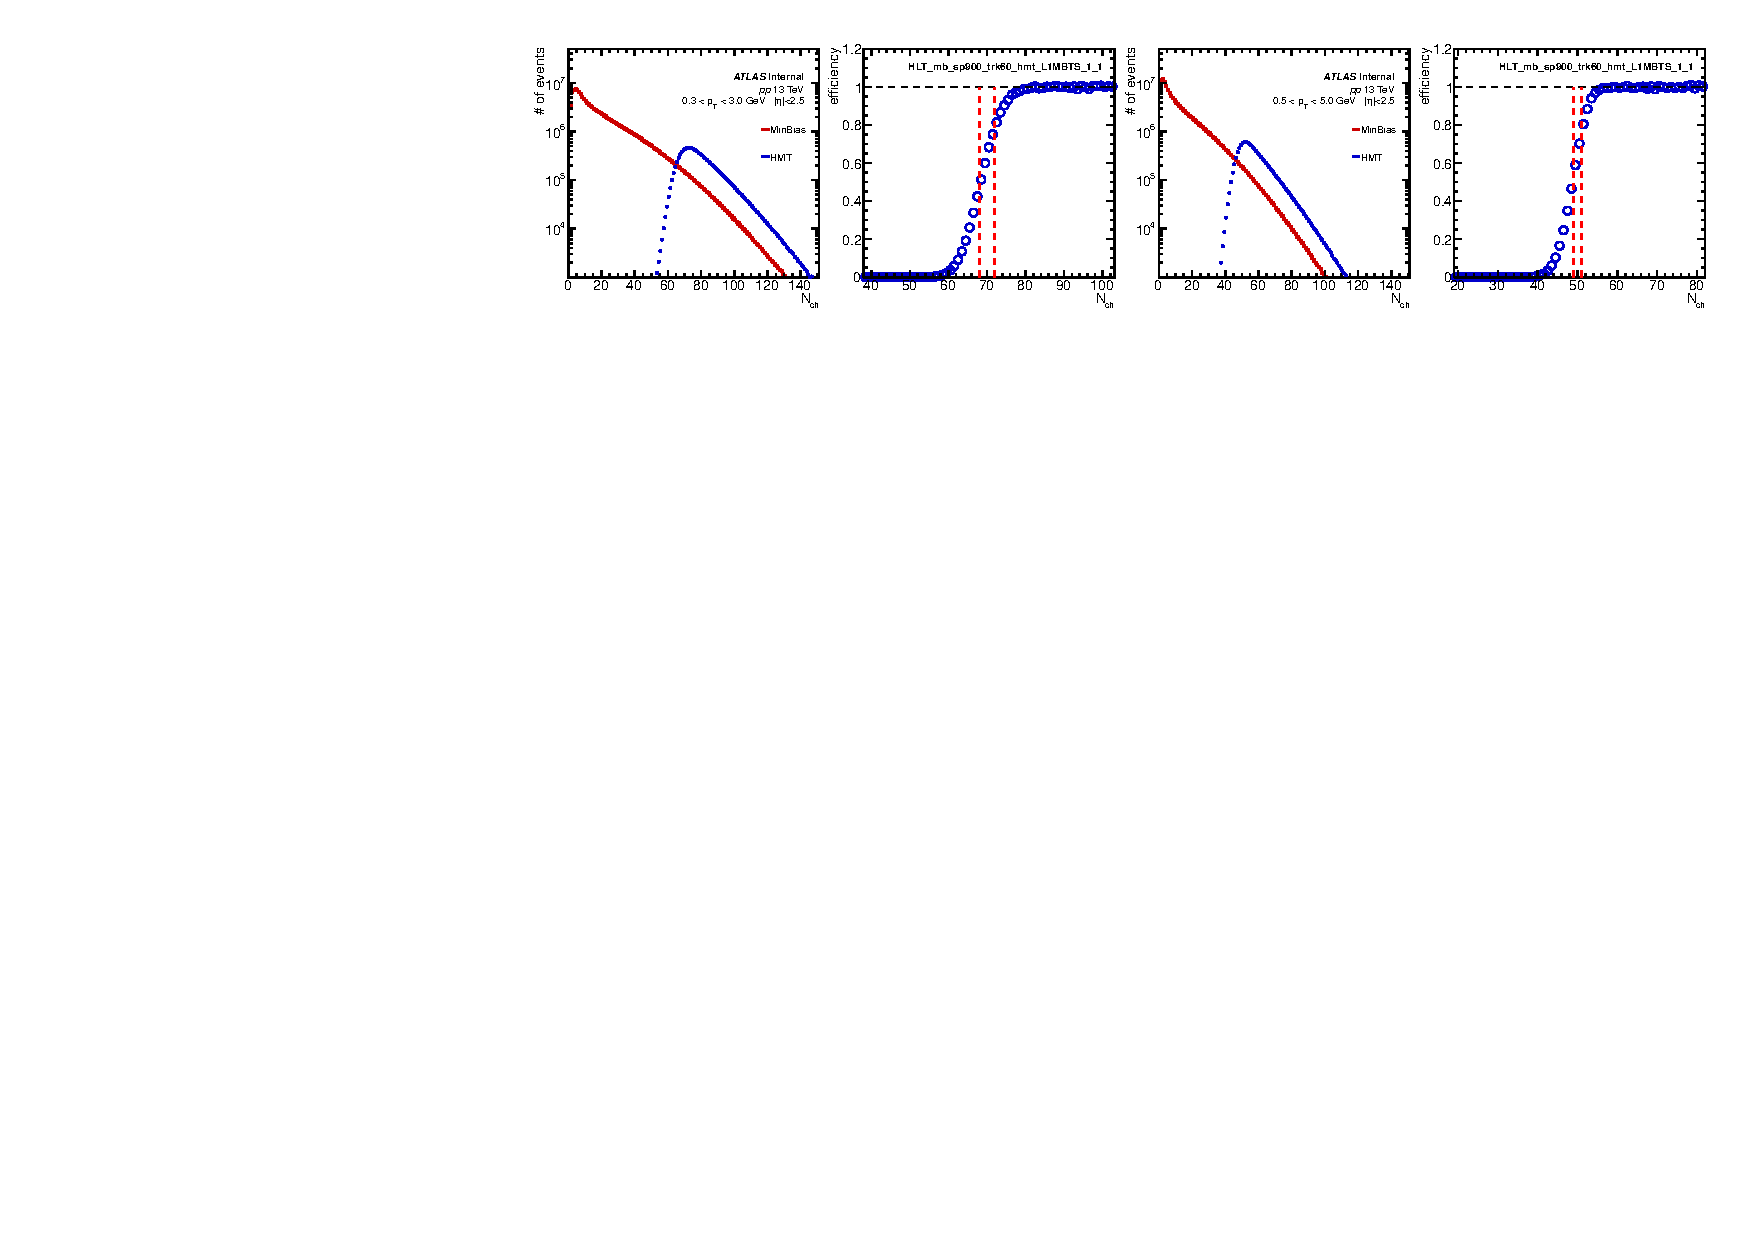
\includegraphics[width=1.\linewidth]{figs/sec_sys/pp13/sys_pp13_trigEff_eg.pdf}
\caption{Trigger efficiencies of one major HMT triggers as a function of number of tracks in two $p_{T}$ ranges: $0.3<p_{T}<3.0$ GeV and $0.5<p_{T}<5.0$ GeV, from 13 TeV $pp$ run period 1. Efficiency is calculated relative to the corresponding MinBias trigger in this run period then scaled to 1.0 in the large $N_{ch}$ region. The two red dash lines indicate 50$\%$ and 80$\%$ efficiency cuts.}
\label{fig:sys_pp13_trigEff_eg}
\end{figure}
Fig.~\ref{fig:sys_pp13_trigEff_eg} shows an example of $N_{ch}$ distribution and efficiency of HMT trigger \verb|HLT_mb_sp900_trk60|, in lower and higher $p_{T}$ ranges separately. The two red dash lines indicate $50\%$ and $80\%$ efficiency cuts. The default trigger efficiency cut is $50\%$ and $80\%$ cut is used as a cross-check. A summary of all the efficiency cuts, together with collected statistics, is shown in table.\ref{table:sys_pp13_trigEff_table}.
\begin{figure}[H]
\centering
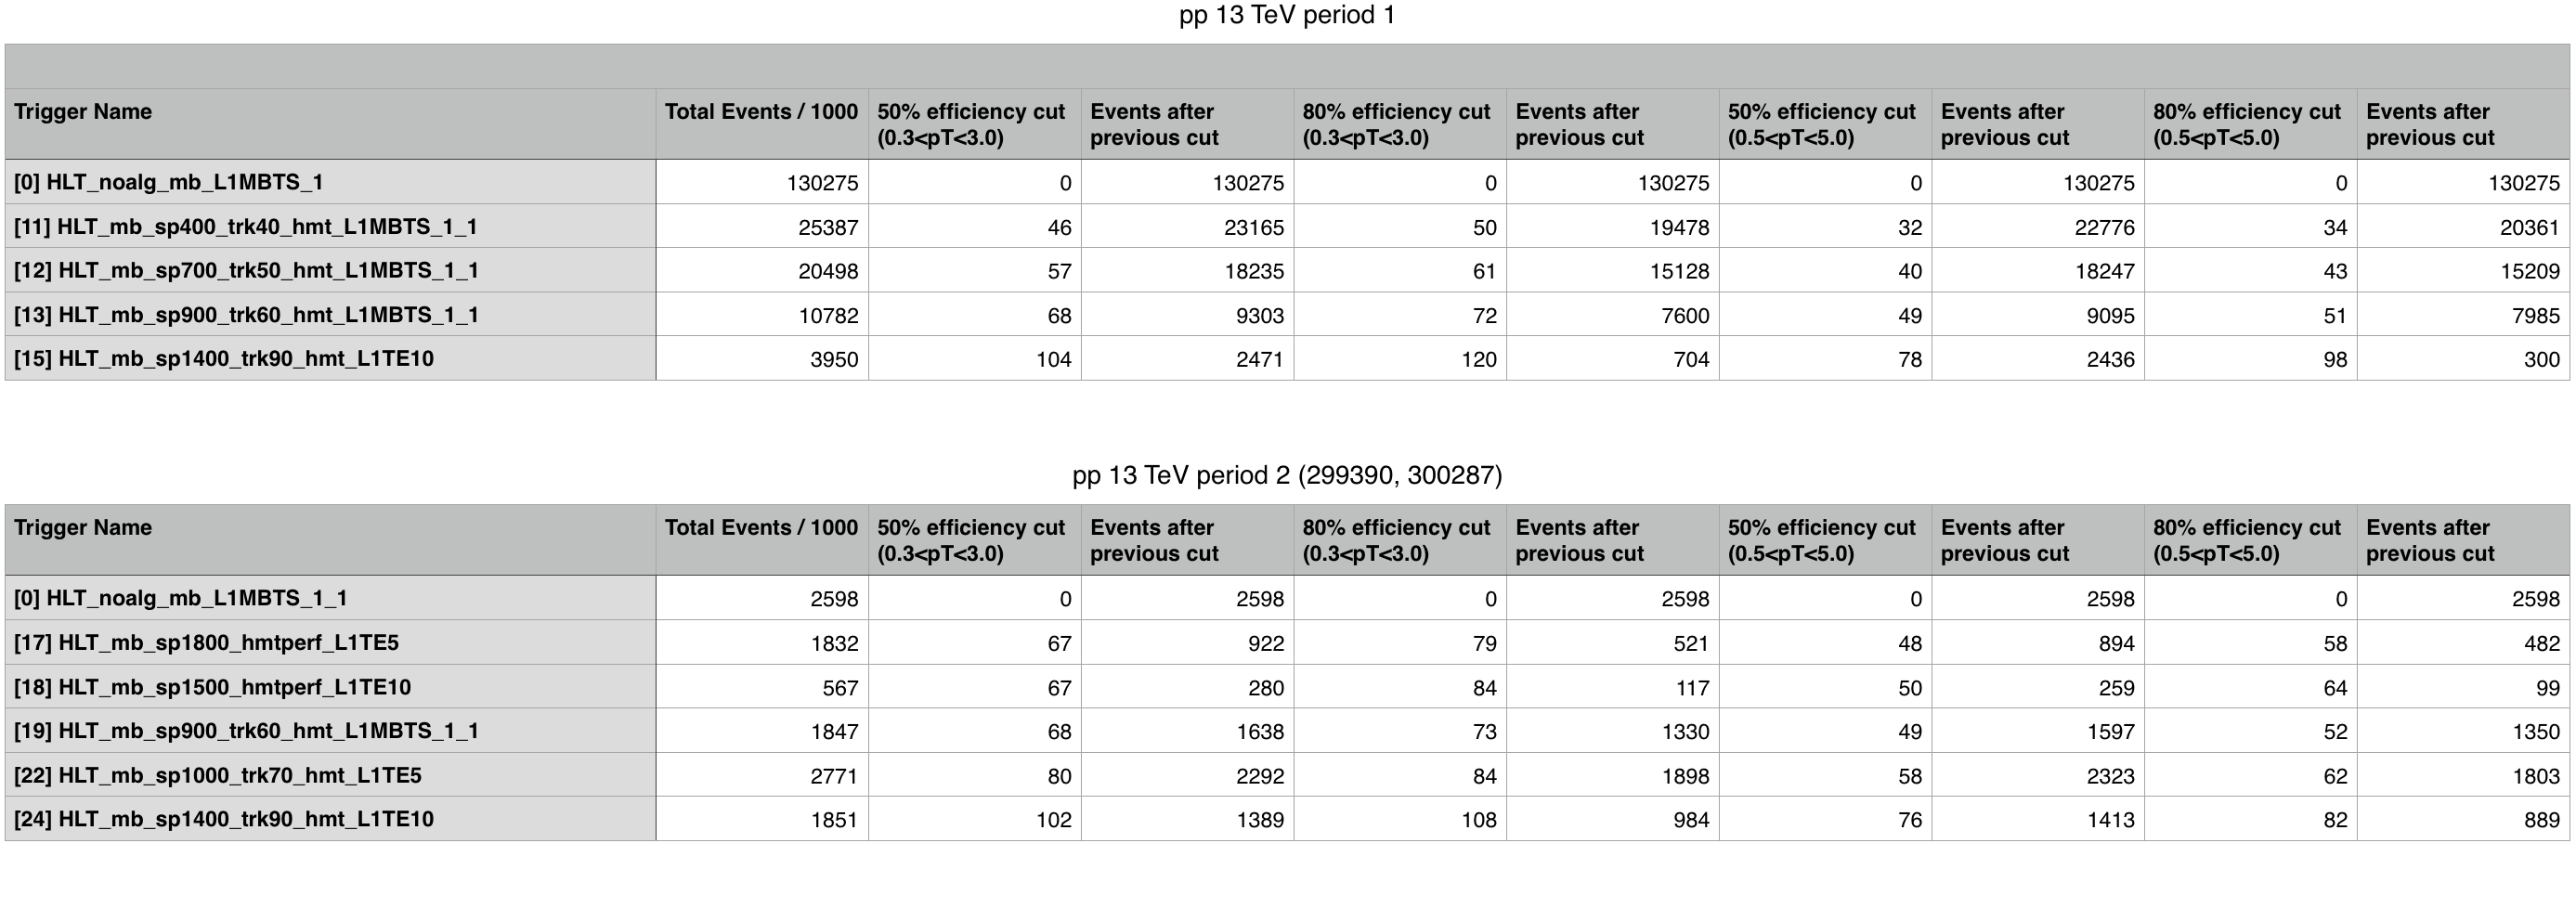
\includegraphics[width=1.\linewidth]{figs/sec_sys/pp13/sys_pp13_trigEff_table_1.png}
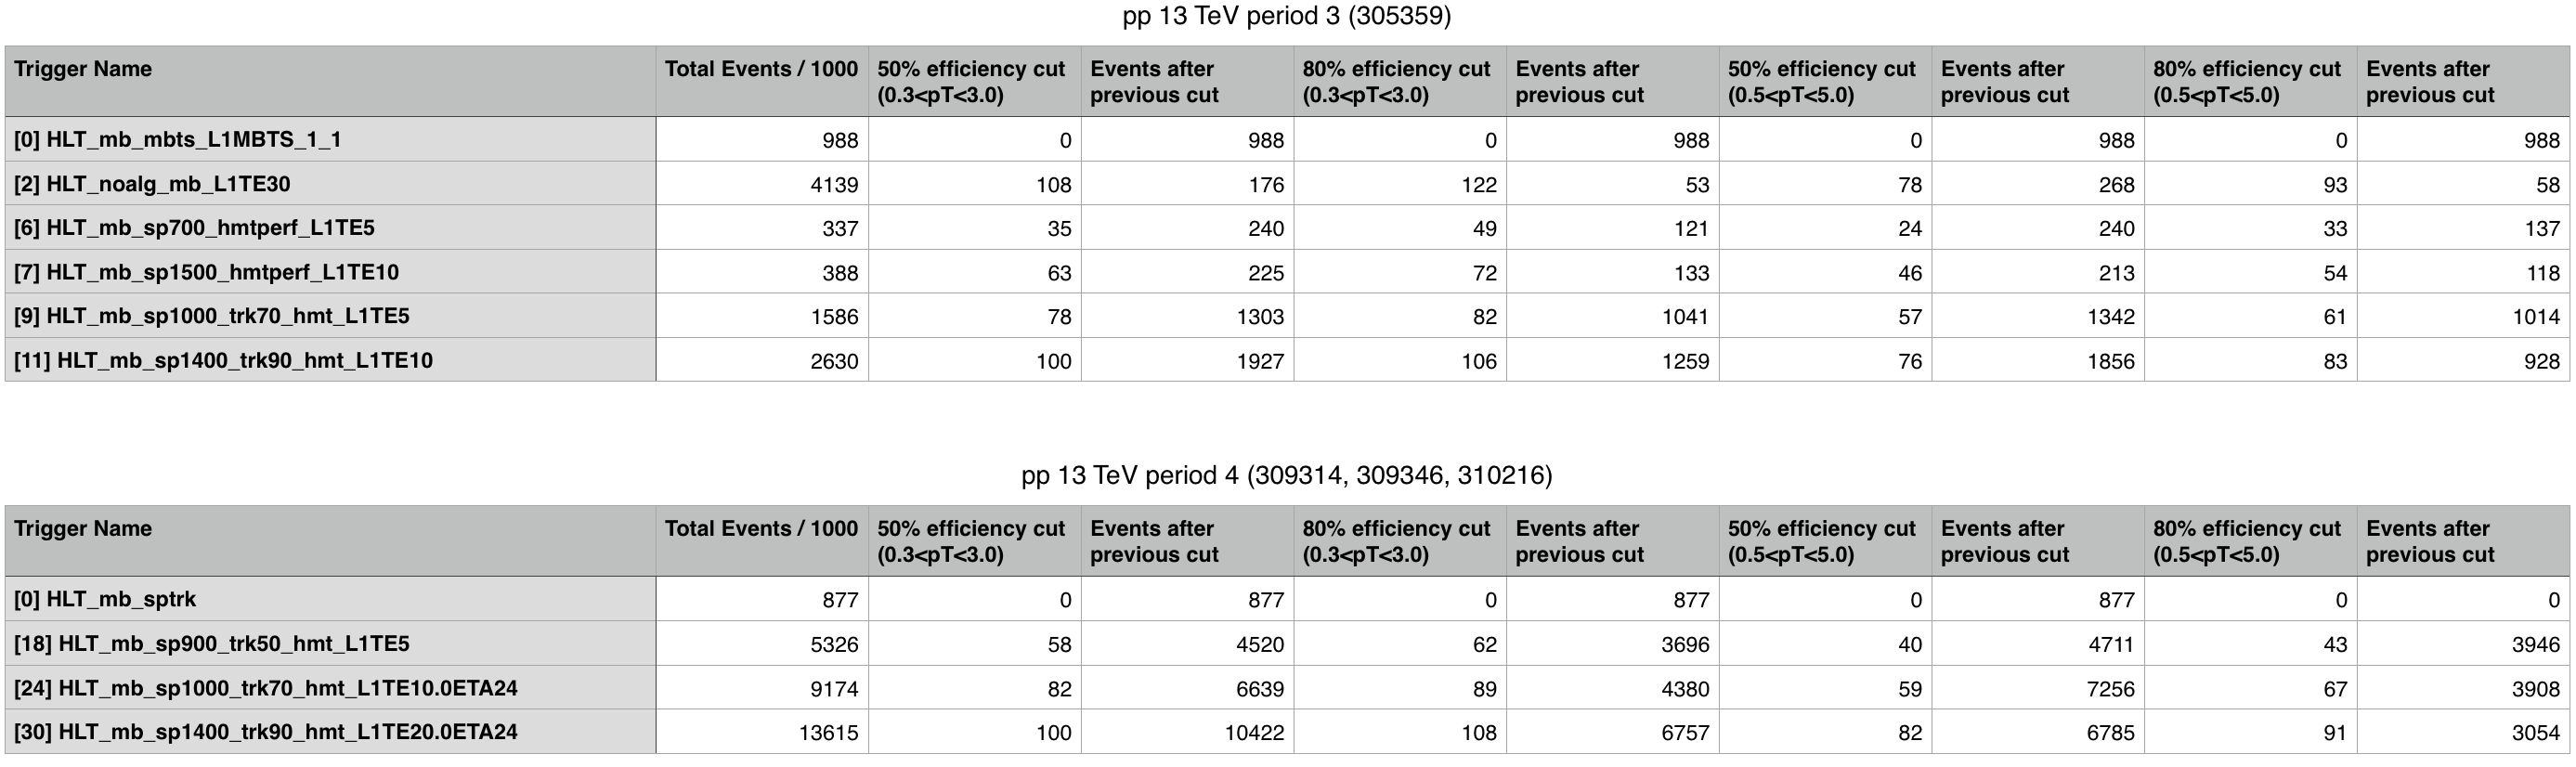
\includegraphics[width=1.\linewidth]{figs/sec_sys/pp13/sys_pp13_trigEff_table_2.png}
\caption{Table of $N_{ch}$ cuts for $50\%$ and $80\%$ trigger efficiencies. The number of events for each trigger after $N_{ch}$ cuts are also listed.}
\label{table:sys_pp13_trigEff_table}
\end{figure}

\begin{figure}[H]
\centering
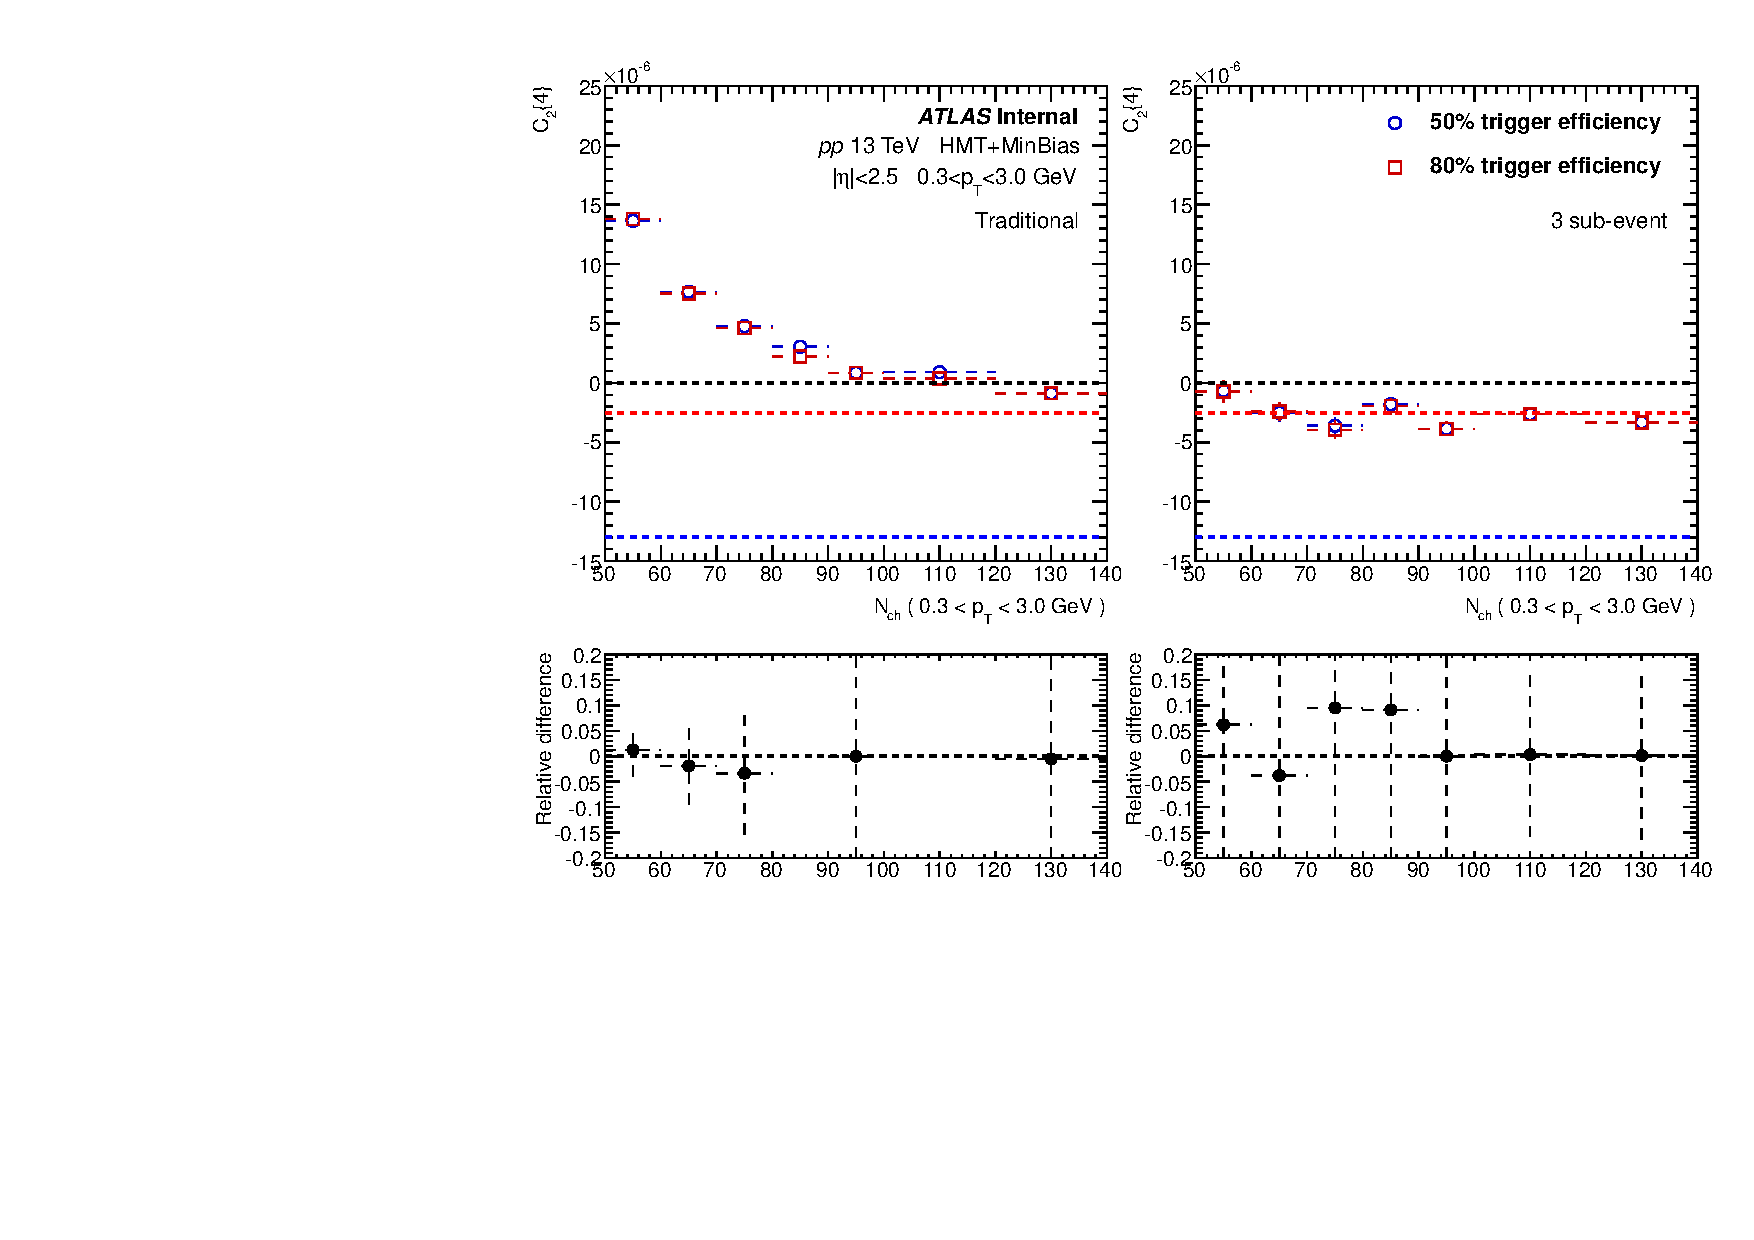
\includegraphics[width=0.8\linewidth]{figs/sec_sys/pp13/sys_pp13_trigEff.pdf}
\caption{$C_{2}\{4\}$ measured with $50\%$ and $80\%$ trigger efficiency cuts. The left column has the results from traditional method and the right column from 3 sub-event method.}
\label{fig:sys_pp13_trigEff}
\end{figure}
Fig.~\ref{fig:sys_pp13_trigEff} shows the $C_{2}\{4\}$ calculated with $50\%$ and $80\%$ trigger efficiency cuts. For the traditional method, the relative difference is on the level of $5\%$, and it goes to larger than $20\%$ when $C_{2}\{4\}$ goes across 0. As a comparison, the relative difference from 3 sub-event method is less than $10\%$ in the region $N_{ch}>50$, and the difference is probably caused by the statistical fluctuation, since 3 sub-event method always has larger statistical error bars. Even with large statistical errors, the relative differences are still quoted as systematic uncertainties.



\subsubsection{Tracking efficiency}
During the offline track reconstruction, not all the tracks will be reconstructed. The fraction of successfully reconstructed tracks are estimated through Monte-Carlo generators with a simulation of ATLAS detector, known as tracking efficiency $\epsilon$. In previous section, the tracking efficiency is evaluated as a function of $\eta$, $p_{T}$ and $N_{ch}$, and while calculating the multi-particle correlations, each particle is weighted by $1/\epsilon$. Since flow is a global quantity and its signal has very weak dependence of $\eta$, the $\eta$ dependence of tracking efficiency should not have a large influence on the results. Furthermore, since the $C_{2}\{4\}$ is measured as a function of $N_{ch}$, this means the only factor that could contribute to the results is the $p_{T}$ weighting in the tracking efficiency. In other words, if tracking efficiency is independent of $p_{T}$, with and without tracking efficiency weight should not cause any difference.

\begin{figure}[H]
\centering
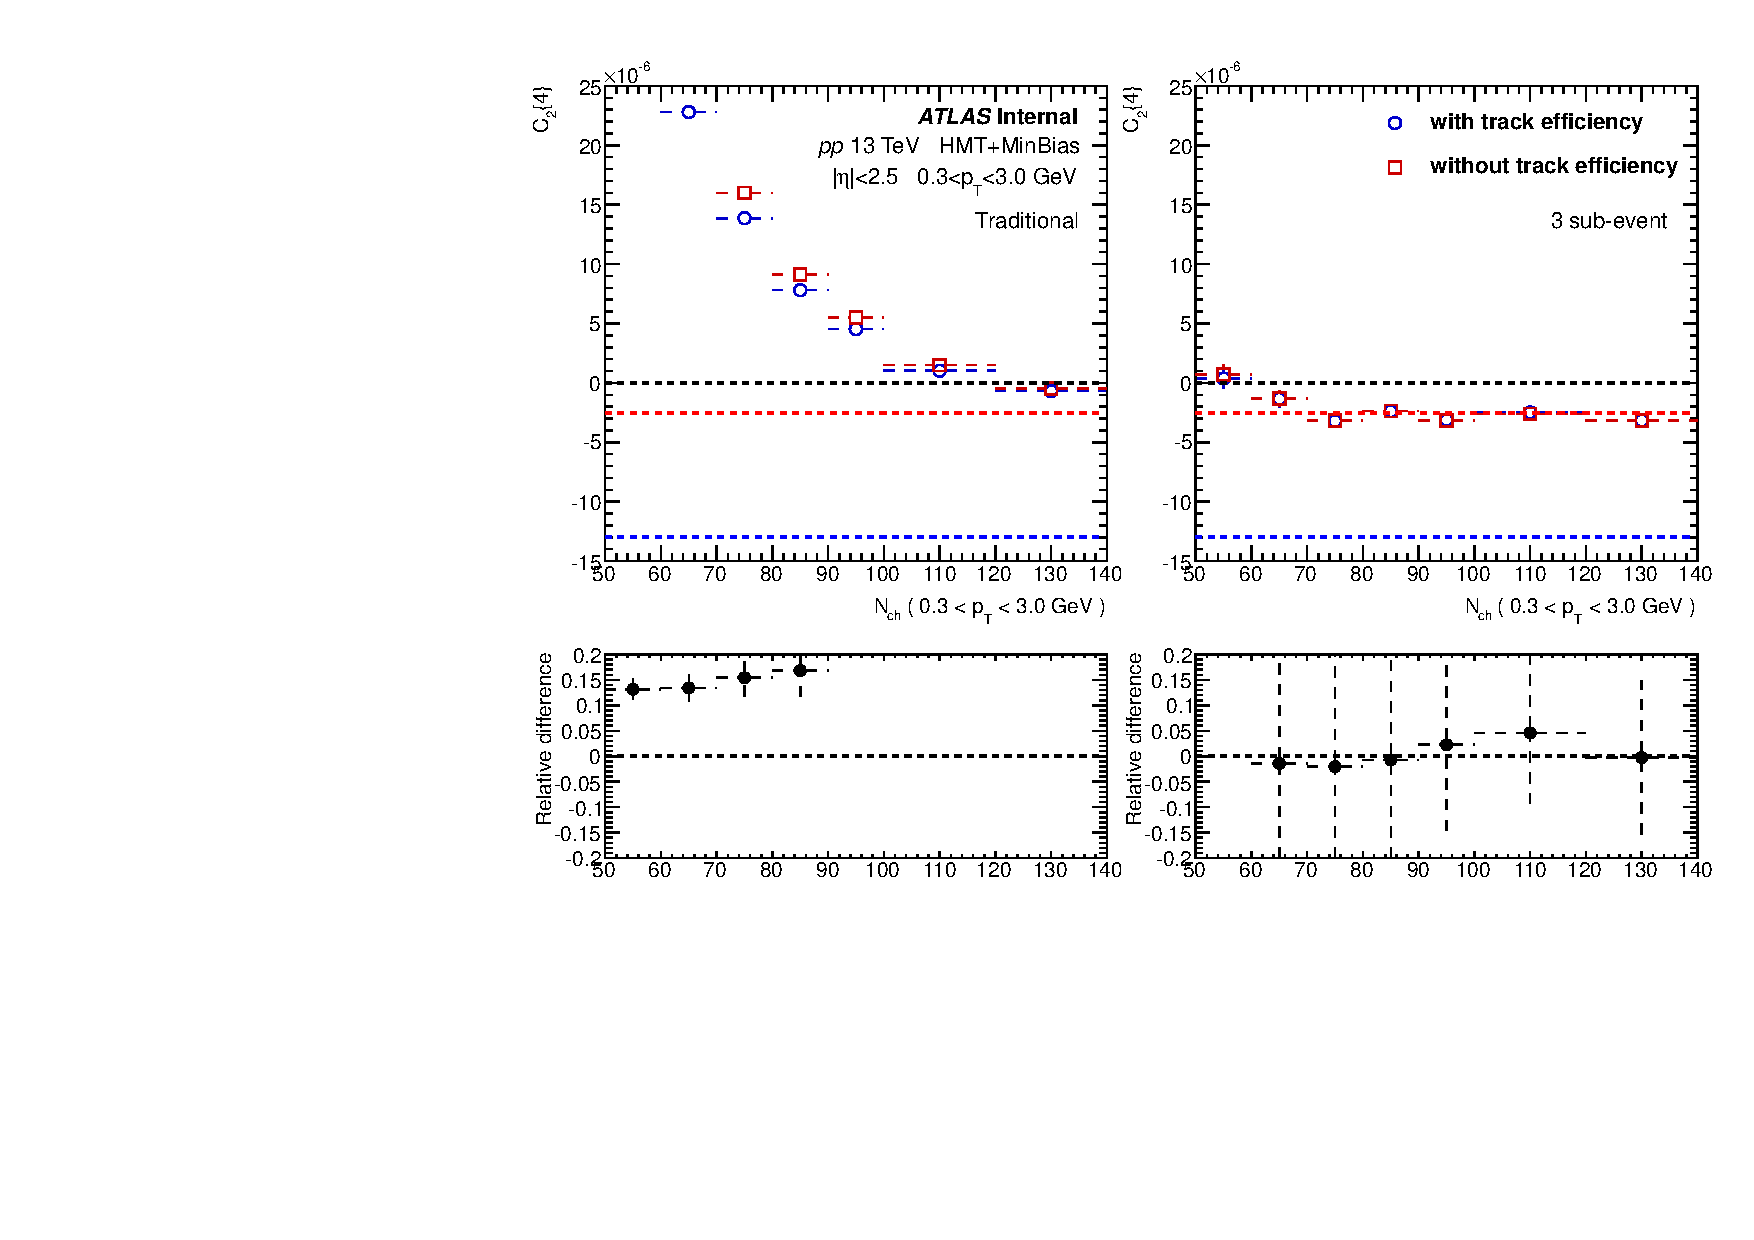
\includegraphics[width=0.8\linewidth]{figs/sec_sys/pp13/sys_pp13_trkEff.pdf}
\caption{$C_{2}\{4\}$ measured with and without tracking efficiency correction. The left column has the results from traditional method and the right column from 3 sub-event method.}
\label{fig:sys_pp13_trkEff}
\end{figure}
Fig.\ref{fig:sys_pp13_trkEff} shows the $C_{2}\{4\}$ calculated with and without tracking efficiency correction. For the traditional method, the relative difference is on the level of $10\%$ larger without efficiency correction and keeps increasing as $N_{ch}$ increases. Meanwhile, the relative difference from 3 sub-event method is less than $5\%$ in the region $N_{ch}>50\%$. As discussed before, what tracking efficiency does is to put different weights to particles with difference $p_{T}$. From many previous flow measurements, it is known that $v_{2}$ usually increases with $p_{T}$ until $p_{T}$ reaches 2-3 GeV, and then decrease. $p_{T}$ dependence of $v_{2}$ is relatively small in the region where tracking efficiency dramatically changes. This means that different $p_{T}$ weighting should have minimal impact on the flow measurement, as been shown in previous $p$+Pb and $Pb+Pb$ results, where with and without tracking efficiency correction does not make a big difference. This explains why with 3 sub-event method, the relative difference is minimal. However, for the traditional method, it is dominated by the non-flow contribution, which might be more sensitive to $p_{T}$ weighting than flow. This could be the reason why traditional method is dependent of tracking efficiency weighting. But in any case, since tracking efficiency correction will introduce additional $p_{T}$ weighting to the results, this check will not be quoted as one of the systematics.

In order to correctly estimate impact from uncertainty of tracking efficiency, the systematic uncertainty on the tracking efficiency in different $|\eta|$ ranges are applied, as shown in Fig.~\ref{fig:sys_pp13_trkEff_sys}. These values are obtained from the 13 TeV multiplicity analysis and include material uncertainties. The entire analysis is re-done by varying the tracking efficiency within its systematic uncertainty. Two extreme cases are chosen:
\begin{itemize}
\item High tracking efficiency: the tracking efficiency is increased by its uncertainty for all $p_{T}$ and $\eta$;
\item Low tracking efficiency: the tracking efficiency is decreased by its uncertainty for all $p_{T}$ and $\eta$.
\end{itemize}

\begin{figure}[H]
\centering
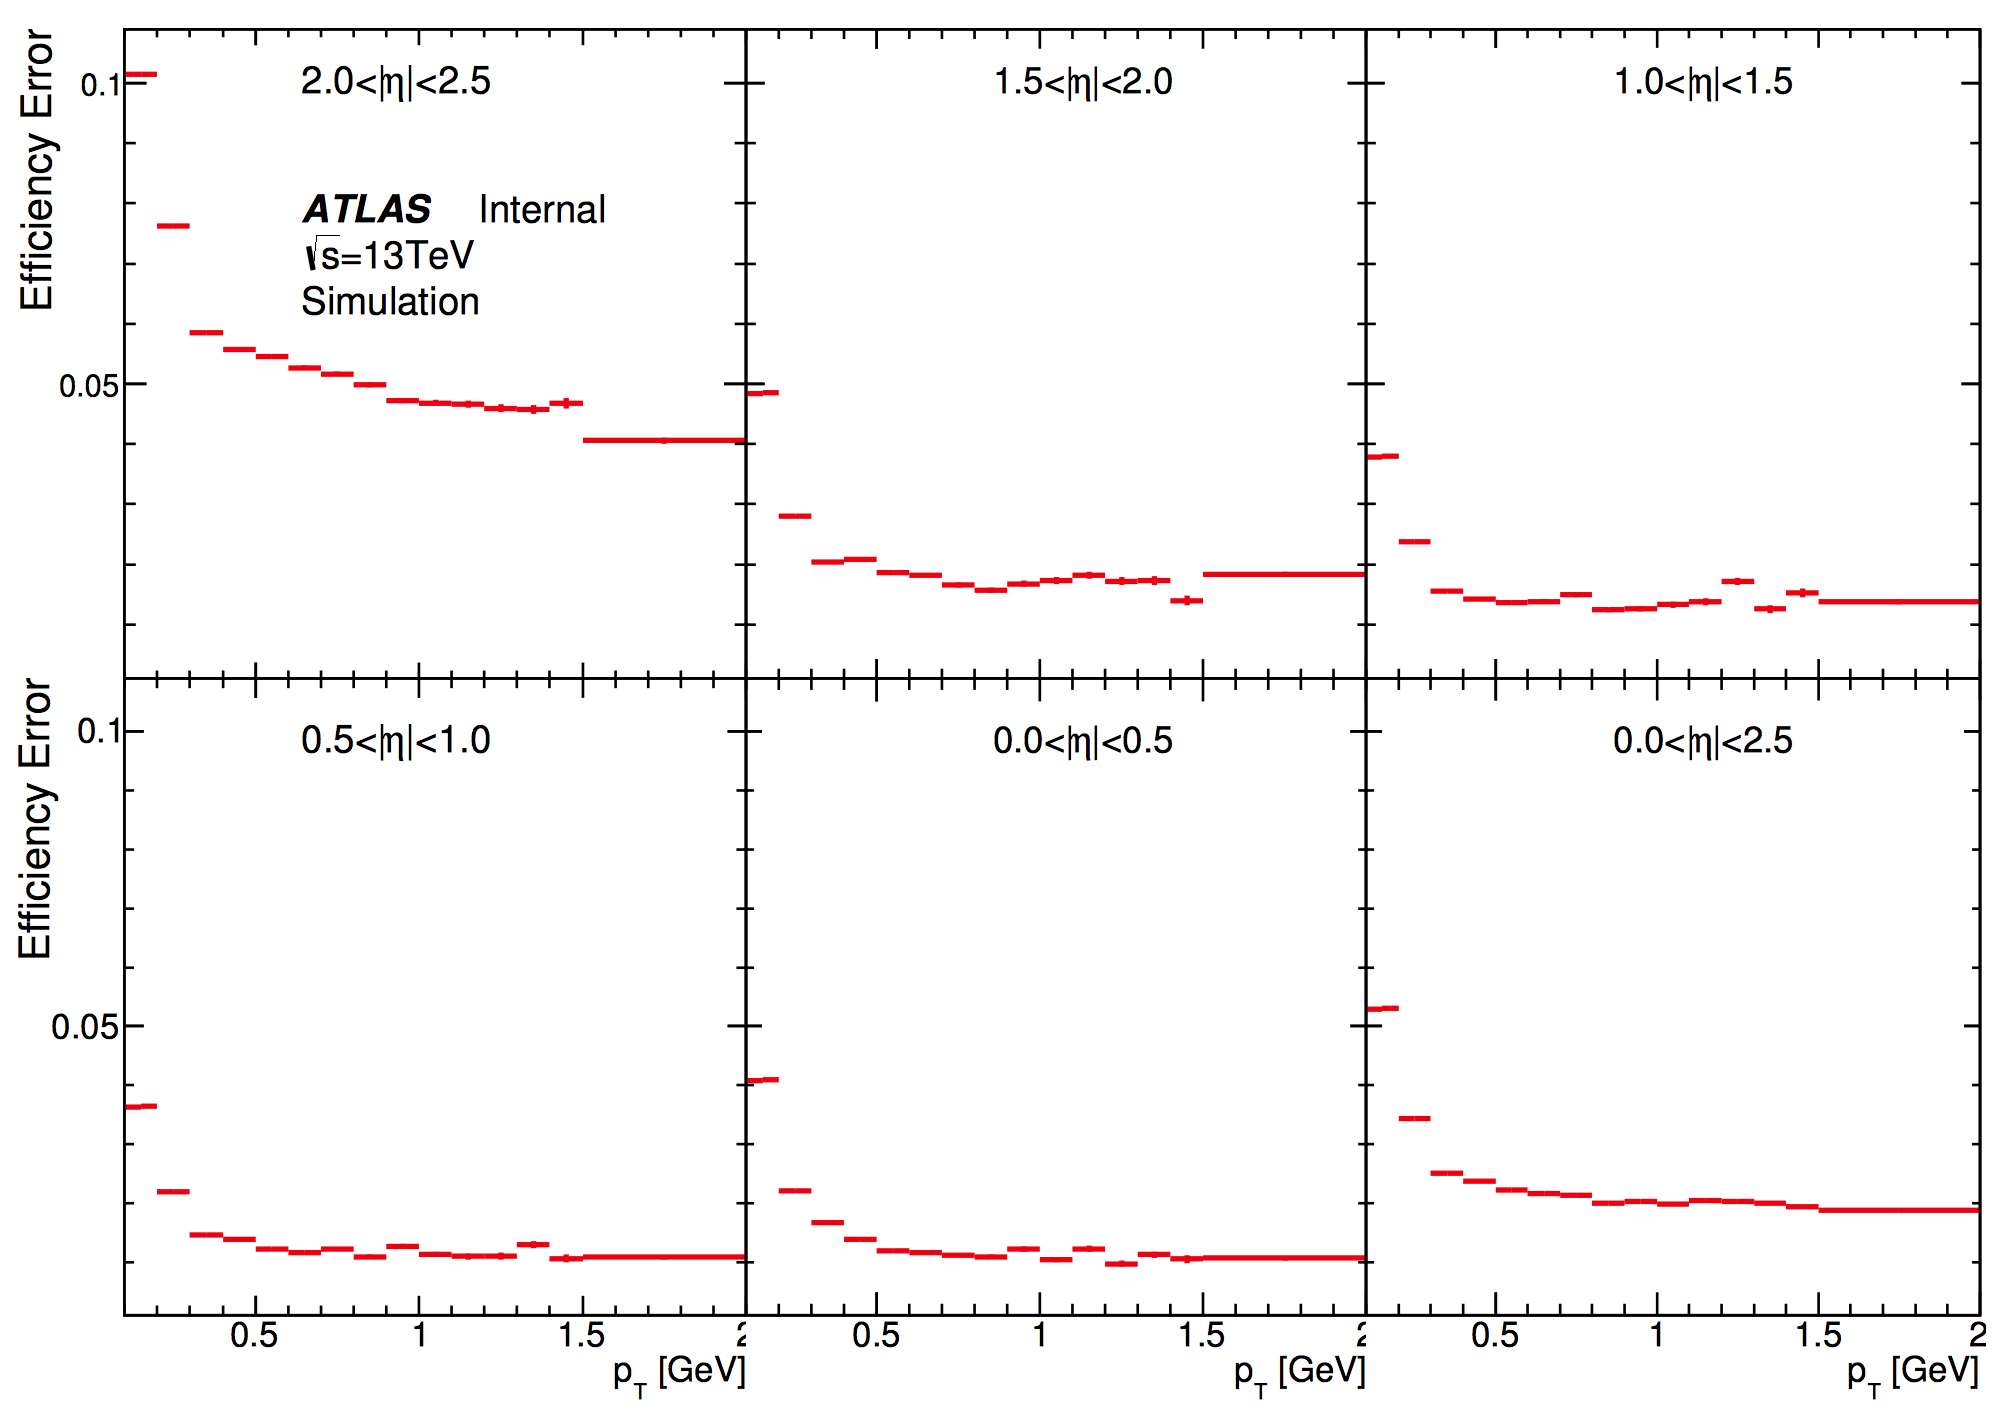
\includegraphics[width=0.8\linewidth]{figs/sec_sys/pp13/sys_pp13_trkEff_sys.png}
\caption{The systematic uncertainties of the tracking efficiency plotted as a function of $p_{T}$ for several $|\eta|$ slices. These include the material uncertainties. These were obtained from the 13TeV multiplicity analysis.}
\label{fig:sys_pp13_trkEff_sys}
\end{figure}
With above variations, the 4-particle cumulant from all three methods are re-evaluated and the results is shown in the summary of systematics.



\subsubsection{Track selection}
Another check is concerning the track selection. The default track selection is listed as follows:
\begin{itemize}
\item Tracks are from primary vertex
\item If IBL hit is expected: at lease 1 IBL hit
\item If on IBL hit is expected: a Layer-0 hit if expected
\item At least 1 pixel hit + dead sensors
\item $p_{T}<300$ MeV: at least 2 SCT hits + dead sensors
\item $p_{T}<400$ MeV: at least 4 SCT hits + dead sensors
\item $p_{T}>400$ MeV: at least 6 SCT hits + dead sensors
\item If $p_{T}>10$ GeV: $\chi^{2}$ probability $<0.01$
\item $|d_{0}|<1.5$
\item $|z_{0}-v_{z}|\text{sin}\theta<1.5$
\item $|\eta|\le 2.5$
\item $p_{T}\ge 200$ MeV
\end{itemize}
and as a check, the track pointing cut is tightened
\begin{itemize}
\item $|d_{0}|<1.0$
\item $|z_{0}-v_{z}|\text{sin}\theta<1.0$
\end{itemize}
while keeping all the rest selection cuts the same. This check will test the stability of results due to the track selection cuts.

\begin{figure}[H]
\centering
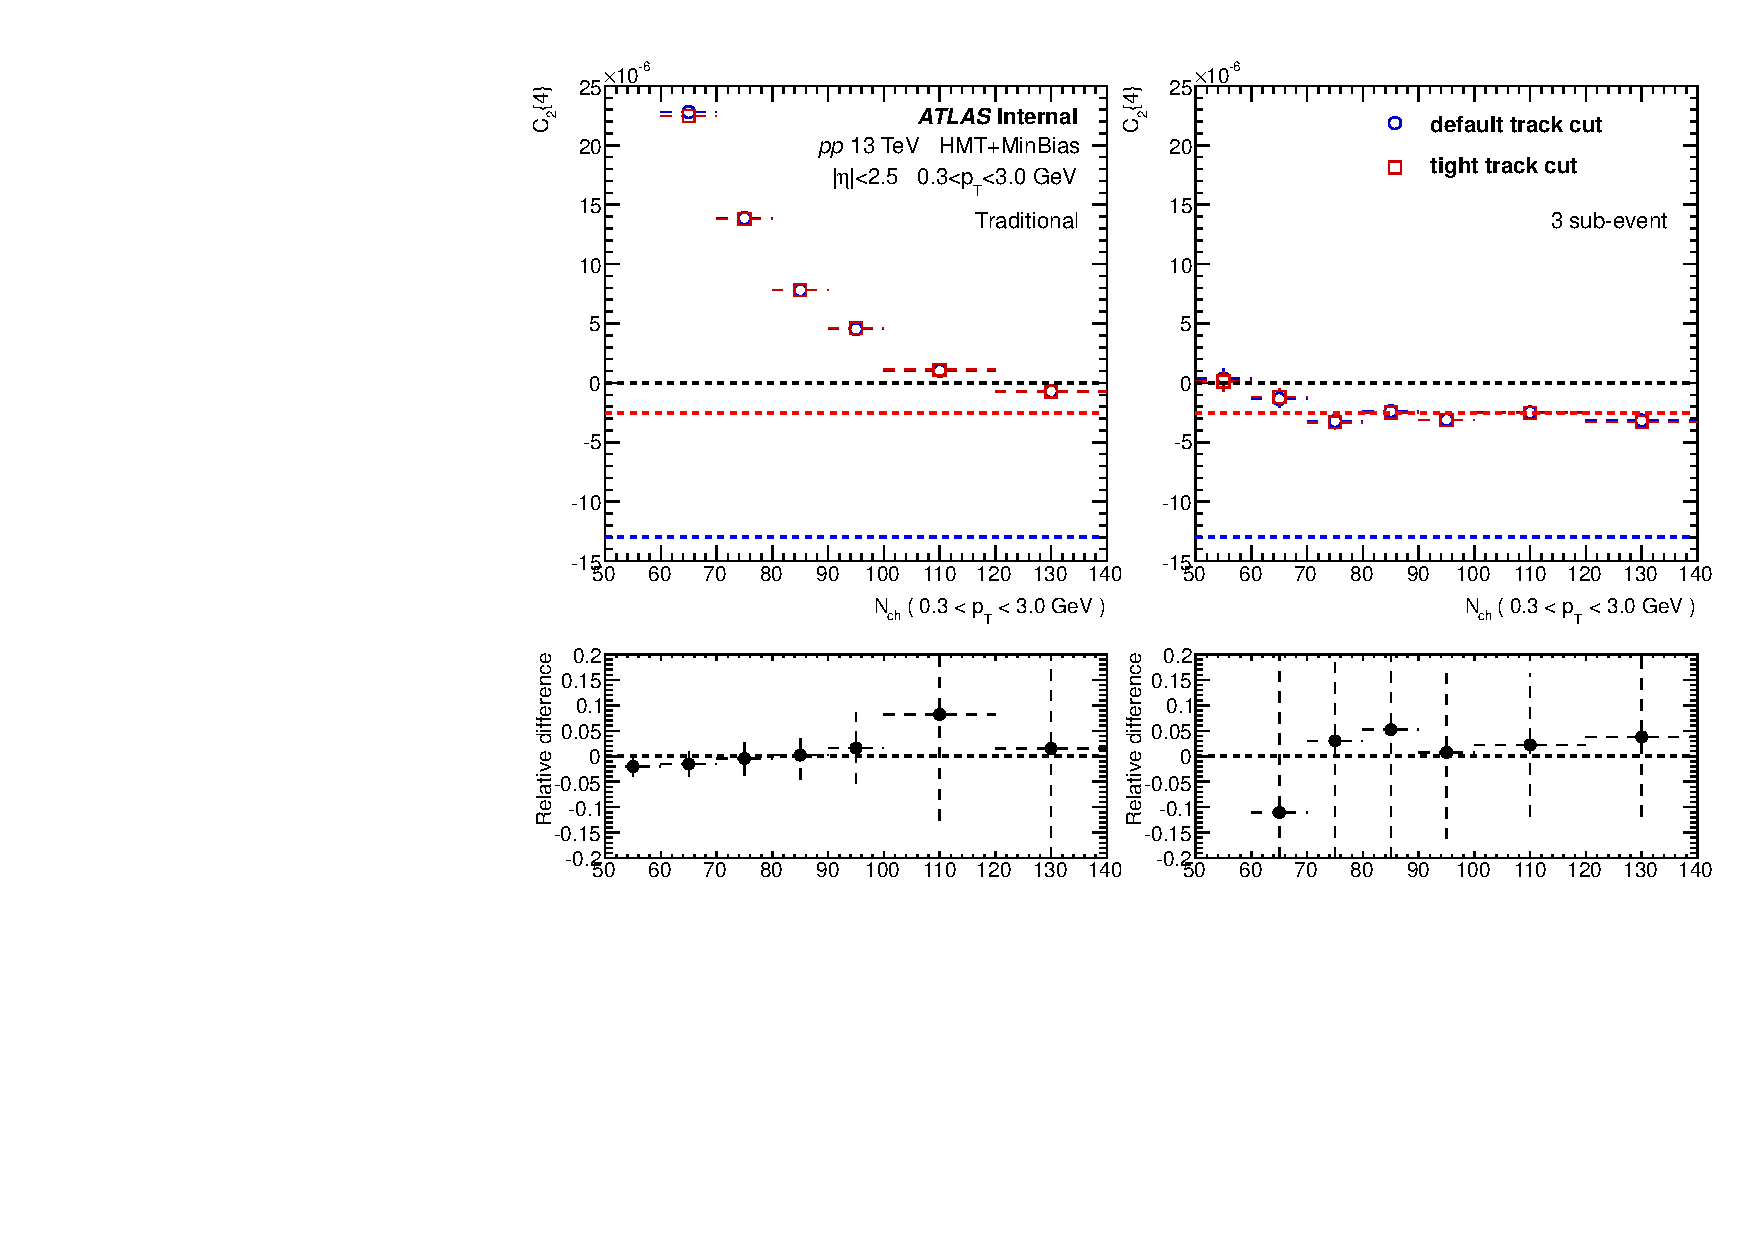
\includegraphics[width=0.8\linewidth]{figs/sec_sys/pp13/sys_pp13_trkSlc.pdf}
\caption{$C_{2}\{4\}$ measured with default and tighter track selection cuts. The left column has the results from traditional method and the right column from 3 sub-event method.}
\label{fig:sys_pp13_trkSlc}
\end{figure}
Fig.\ref{fig:sys_pp13_trkSlc} shows the $C_{2}\{4\}$ calculated with default and tighter track selection cuts. It is obvious that both traditional and 3 sub-event methods have minimal dependence of track selection. This is not hard to interpret since the tighter cuts only reject less than $<1\%$ of the tracks, and such loss is compensated by the tracking efficiency. This check will be quoted as one of the systematics.



\subsubsection{Pile-up condition}
In this analysis all the tracks used to calculate cumulants are from the primary vertex. In principle, in pile-up events, tracks from pile-up vertex should not contribute to the measurement. However, during the track and vertex reconstruction, when a pile-up vertex is too close to the primary vertex, two vertices might be merged. Since the particles from two different vertices are totally uncorrelated, including these events with pile-up vertex will reduce the signal of flow signal.

13 TeV $pp$ runs have 4 run periods, and the $\mu$ values varies from 0.003 to 0.6. In order to estimate how pile-up will affect the results, the whole data sample is divided into 2 sub-sample:
\begin{itemize}
\item Runs with peak $\mu<0.4$;
\item Runs with peak $\mu>0.4$;
\end{itemize}
and the $\mu$ value across all the runs are summarized in table.~\ref{table:sys_pp13_pileUp_table}. The threshold $\mu=0.4$ is chosen so that the statistics in two run groups are roughly the same. In the table, runs tagged with green are the runs with relatively low-$\mu$ and runs tagged with red are with relatively high-$\mu$.
\begin{figure}[H]
\centering
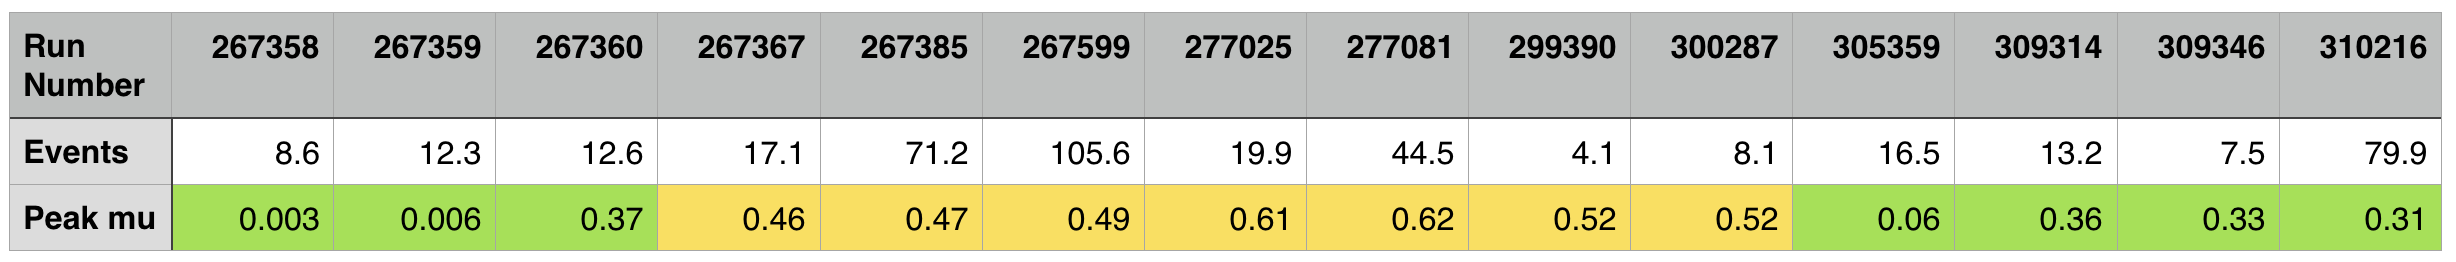
\includegraphics[width=1.0\linewidth]{figs/sec_sys/pp13/sys_pp13_pileUp_table.png}
\caption{Table showing the $\mu$ value and statistics in all the runs from 13 TeV $pp$. Runs tagged with green are the runs with relatively low-$\mu$ and runs tagged with red are with relatively high-$\mu$.}
\label{table:sys_pp13_pileUp_table}
\end{figure}

\begin{figure}[H]
\centering
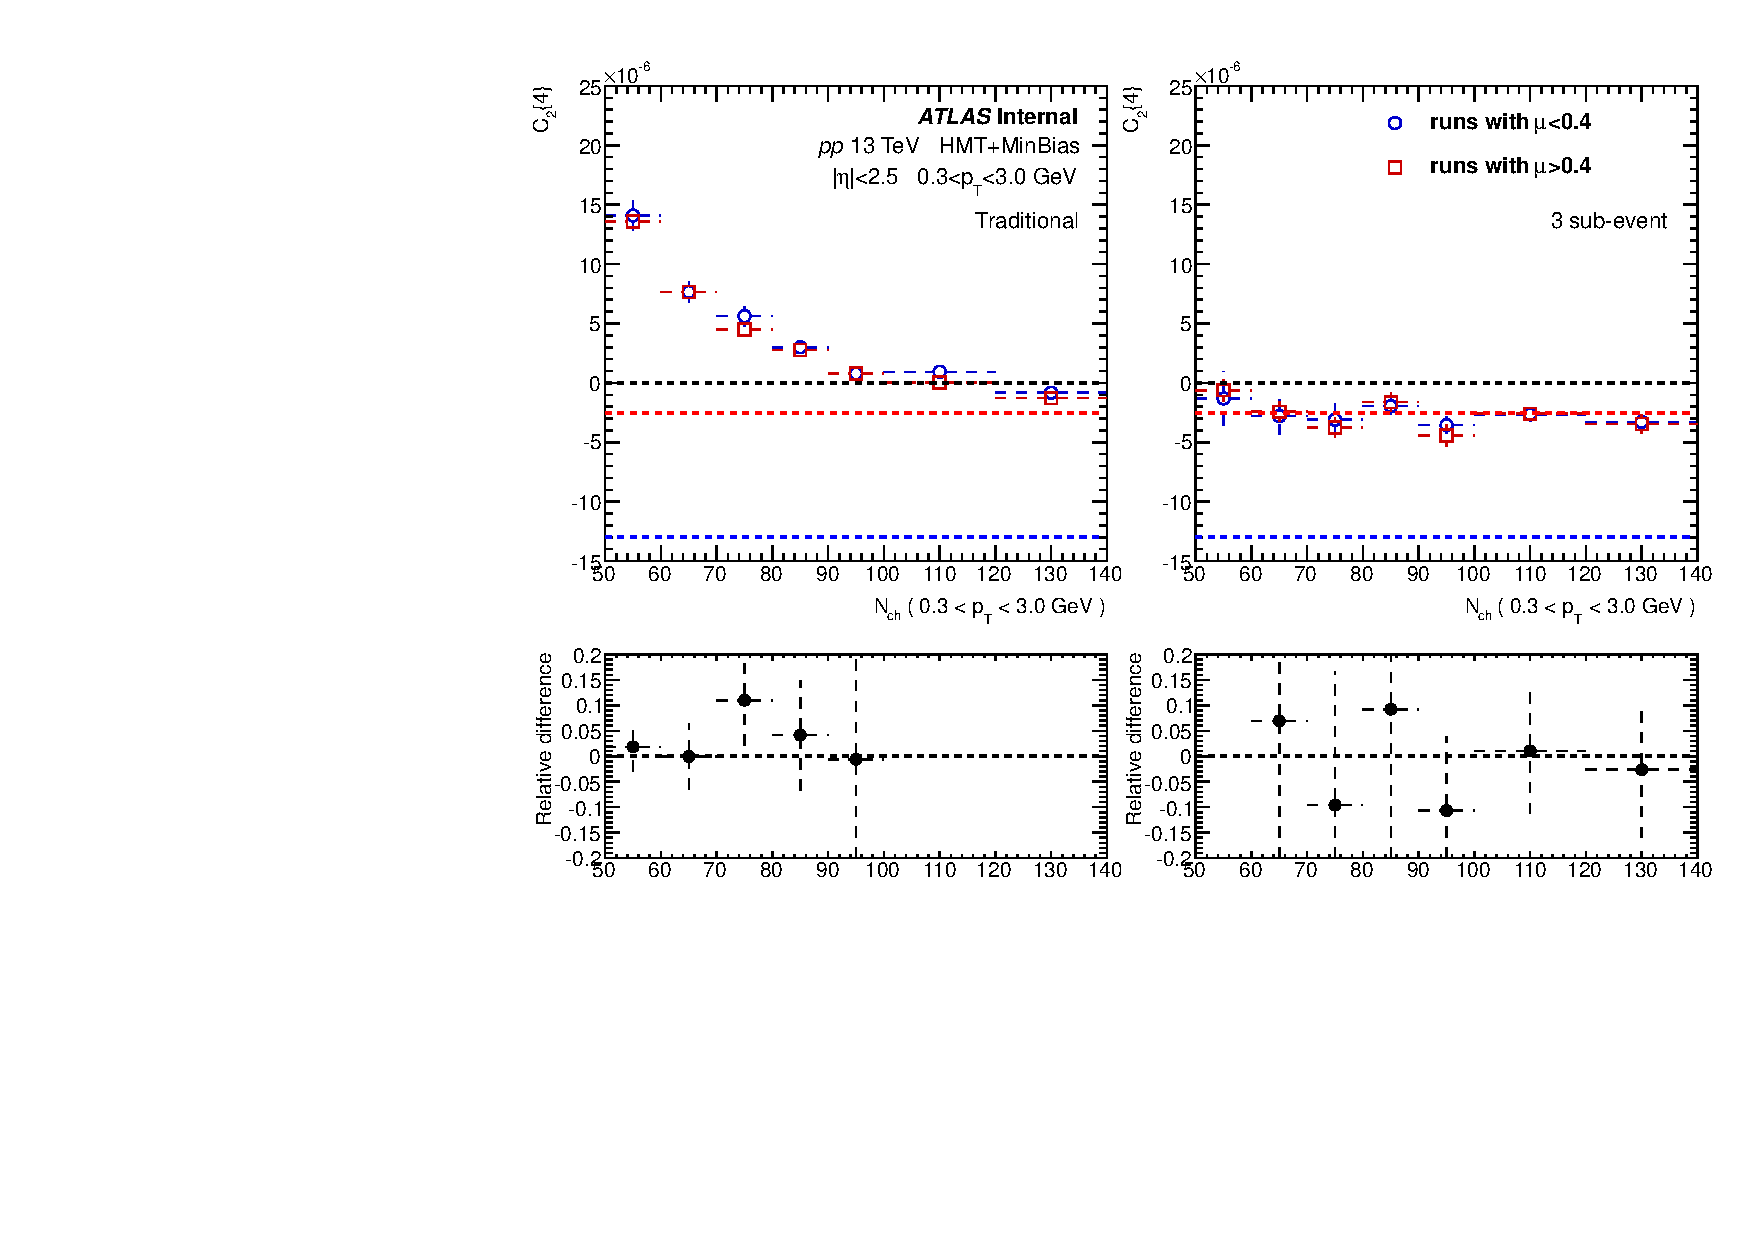
\includegraphics[width=0.8\linewidth]{figs/sec_sys/pp13/sys_pp13_pileUp.pdf}
\caption{$C_{2}\{4\}$ measured in two run groups with different $\mu$ values. The left column has the results from traditional method and the right column from 3 sub-event method.}
\label{fig:sys_pp13_pileUp}
\end{figure}
Since in this check the whole data set is divided into two run groups, which means the statistical fluctuation is larger than previous check, which is reflected in the results. In both traditional and 3 sub-event cumulant results, relative differences are fluctuating around 0, meaning the differences are dominated by the statistical fluctuation. Under this circumstance, we will re-bin the X-axis to increase the statistical significance. The merged results will be shown in the summary of systematics.



\subsubsection{Residual detector effects}
Tracking efficiency weighting corrects the possible detector effects as a function of $\eta$ and $p_{T}$, but the residual detector effects could still remain in the $\phi$ direction. In $pp$ collision, since the "event plane" angle differs from one event to another, the $\phi$ distribution over many events should be flat and the discrepancy upon that is caused by the residual detector effects.

\begin{figure}[H]
\centering
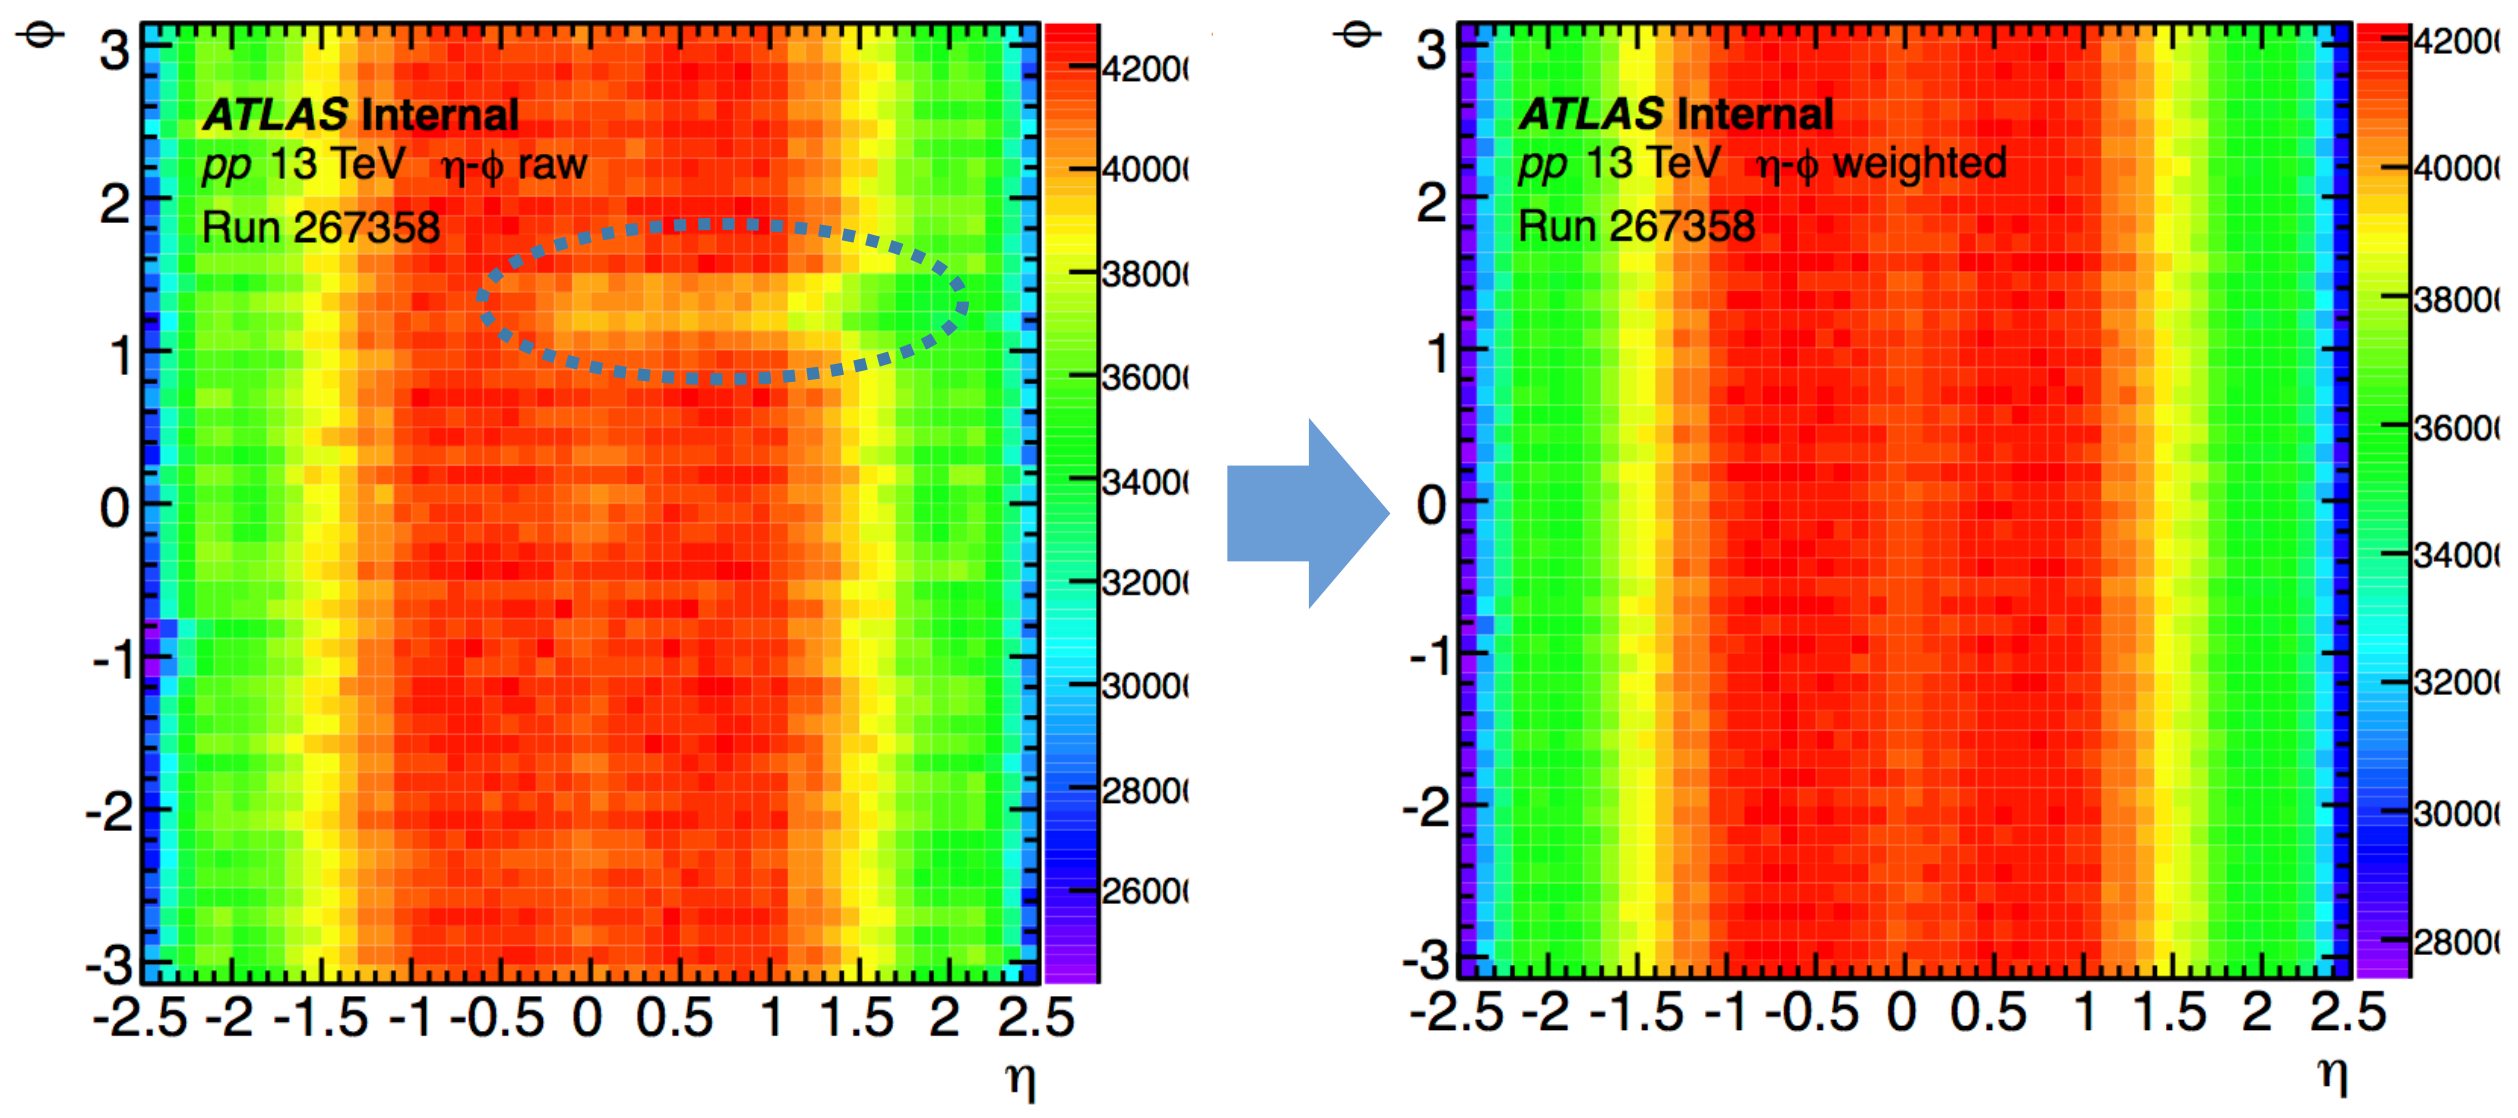
\includegraphics[width=0.8\linewidth]{figs/sec_sys/pp13/sys_pp13_flat_eg.png}
\caption{An example of $\eta-\phi$ distribution of all the events in one run. Left plot is the raw distribution, and right plot is after the correction.}
\label{fig:sys_pp13_flat_eg}
\end{figure}
In order to show this, Fig.~\ref{fig:sys_pp13_flat_eg} presents one example of $\eta-\phi$ distribution of all the events in one run. Left plot is the raw distribution, where some discrepancy has been observed (circled in blue). In order to correct this detector effect, an additional weighting has been applied to the particles while calculating the multi-particle correlation:
\begin{equation}
w_{\phi}(\eta,\phi)\equiv \frac{\lr{N(\delta\eta)}}{N(\delta\eta,\delta\phi)}
\end{equation}
and after the correlation, by construction, the $\eta-\phi$ map becomes flat in $\phi$. This procedure has been used in many other flow analyses and known as "flattening". Since the detector condition could vary from run to run, $w_{\phi}$ is calculated run-by-run and the summary is shown in the data analysis section.

\begin{figure}[H]
\centering
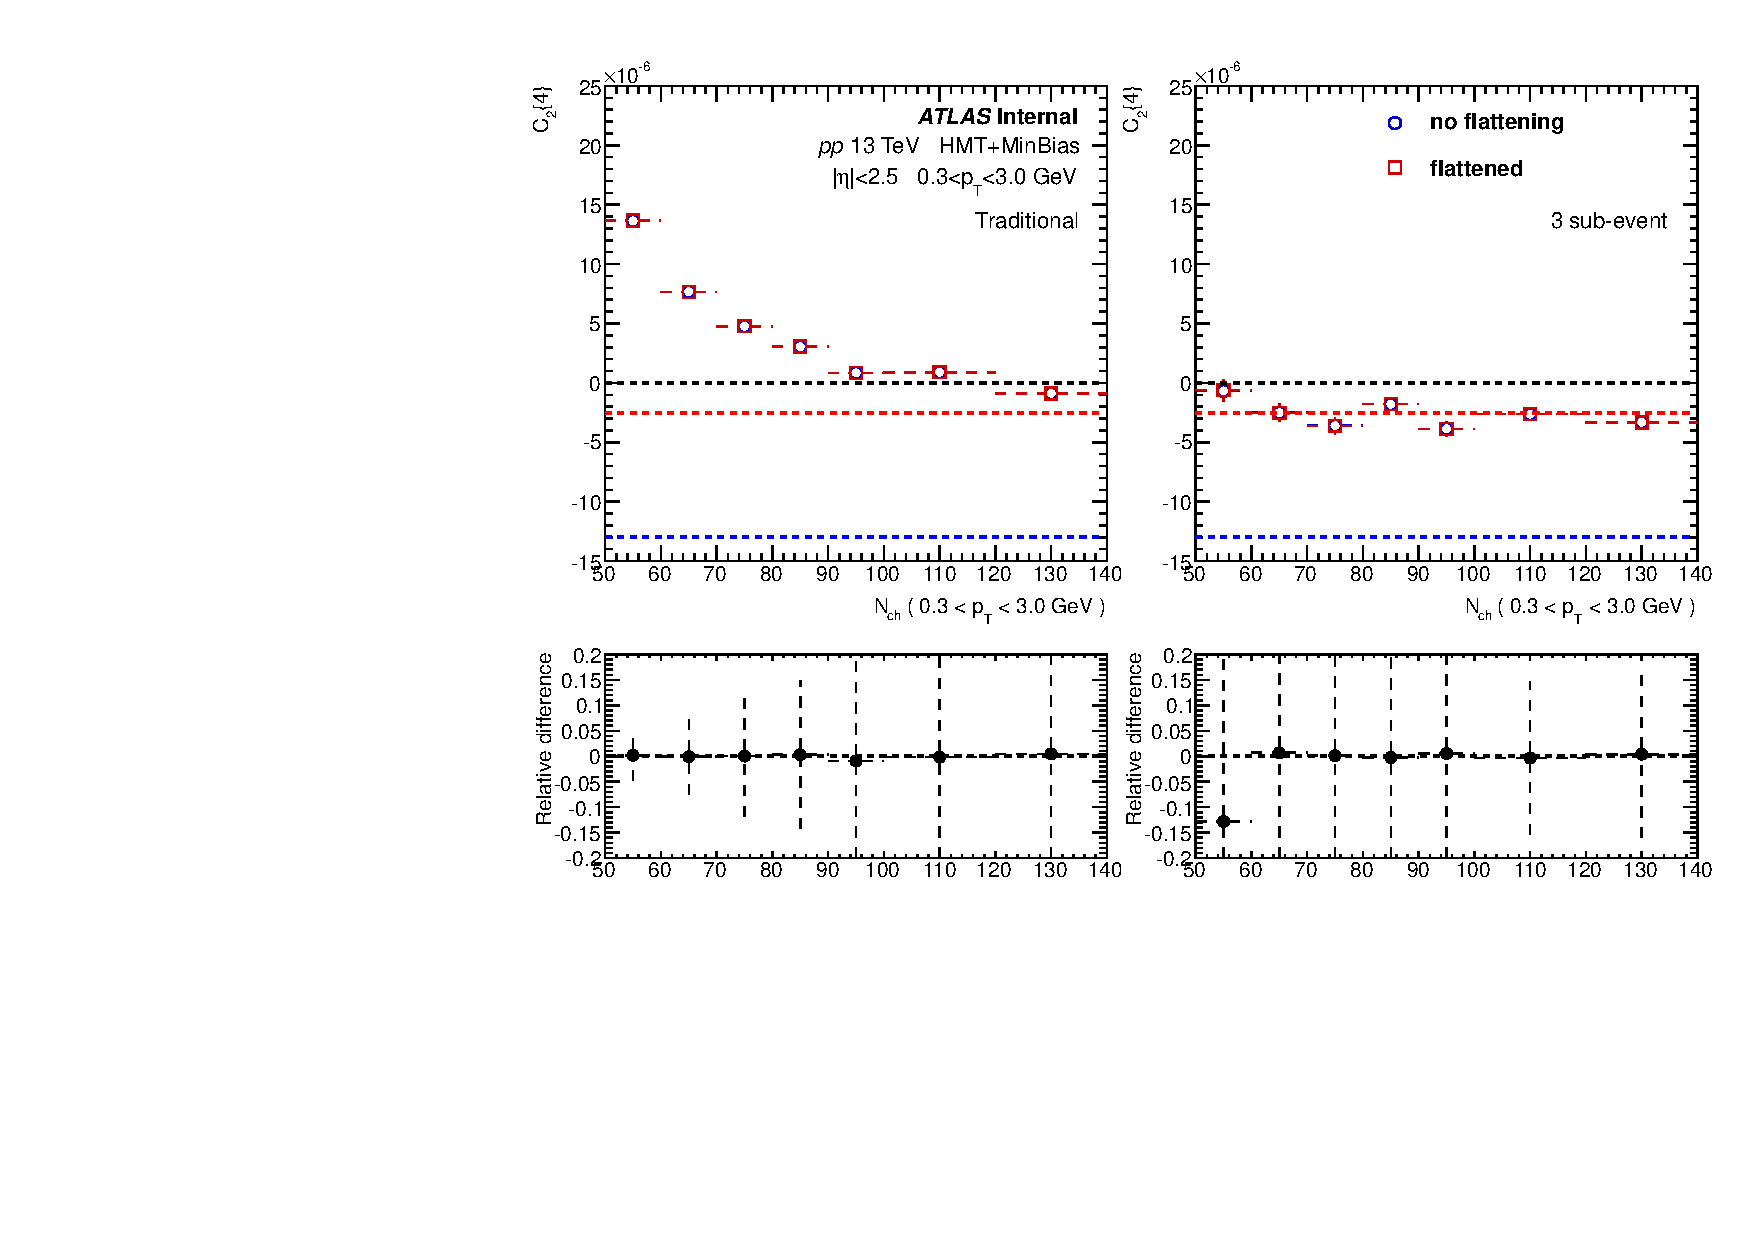
\includegraphics[width=0.8\linewidth]{figs/sec_sys/pp13/sys_pp13_flat.pdf}
\caption{$C_{2}\{4\}$ measured with and without correcting the residual detector effects. The left column has the results from traditional method and the right column from 3 sub-event method.}
\label{fig:sys_pp13_flat}
\end{figure}
Fig.~\ref{fig:sys_pp13_flat} compares the $C_{2}\{4\}$ with and without flattening procedure. For both methods, the relative differences are within $1\%$, meaning such residual detector effects have minimal influence on the results. This check will be quoted as one of the systematics.


\subsubsection{Event class bin width}
As has been discussed before, traditional cumulant is sensitive to the multiplicity fluctuation, which is originated from the observation that non-flow fluctuation is changed when combining different events into groups. For this reason, while calculating the cumulant, the events are always binned with 1 $N_{ch}$ bin width, and the particles used for event class definition are the same as particles used in cumulant calculation. In the results section, we will discuss the influence of using particles with different $p_{T}$ for event class definition. Here we will discuss another factor: event class bin width.

\begin{figure}[H]
\centering
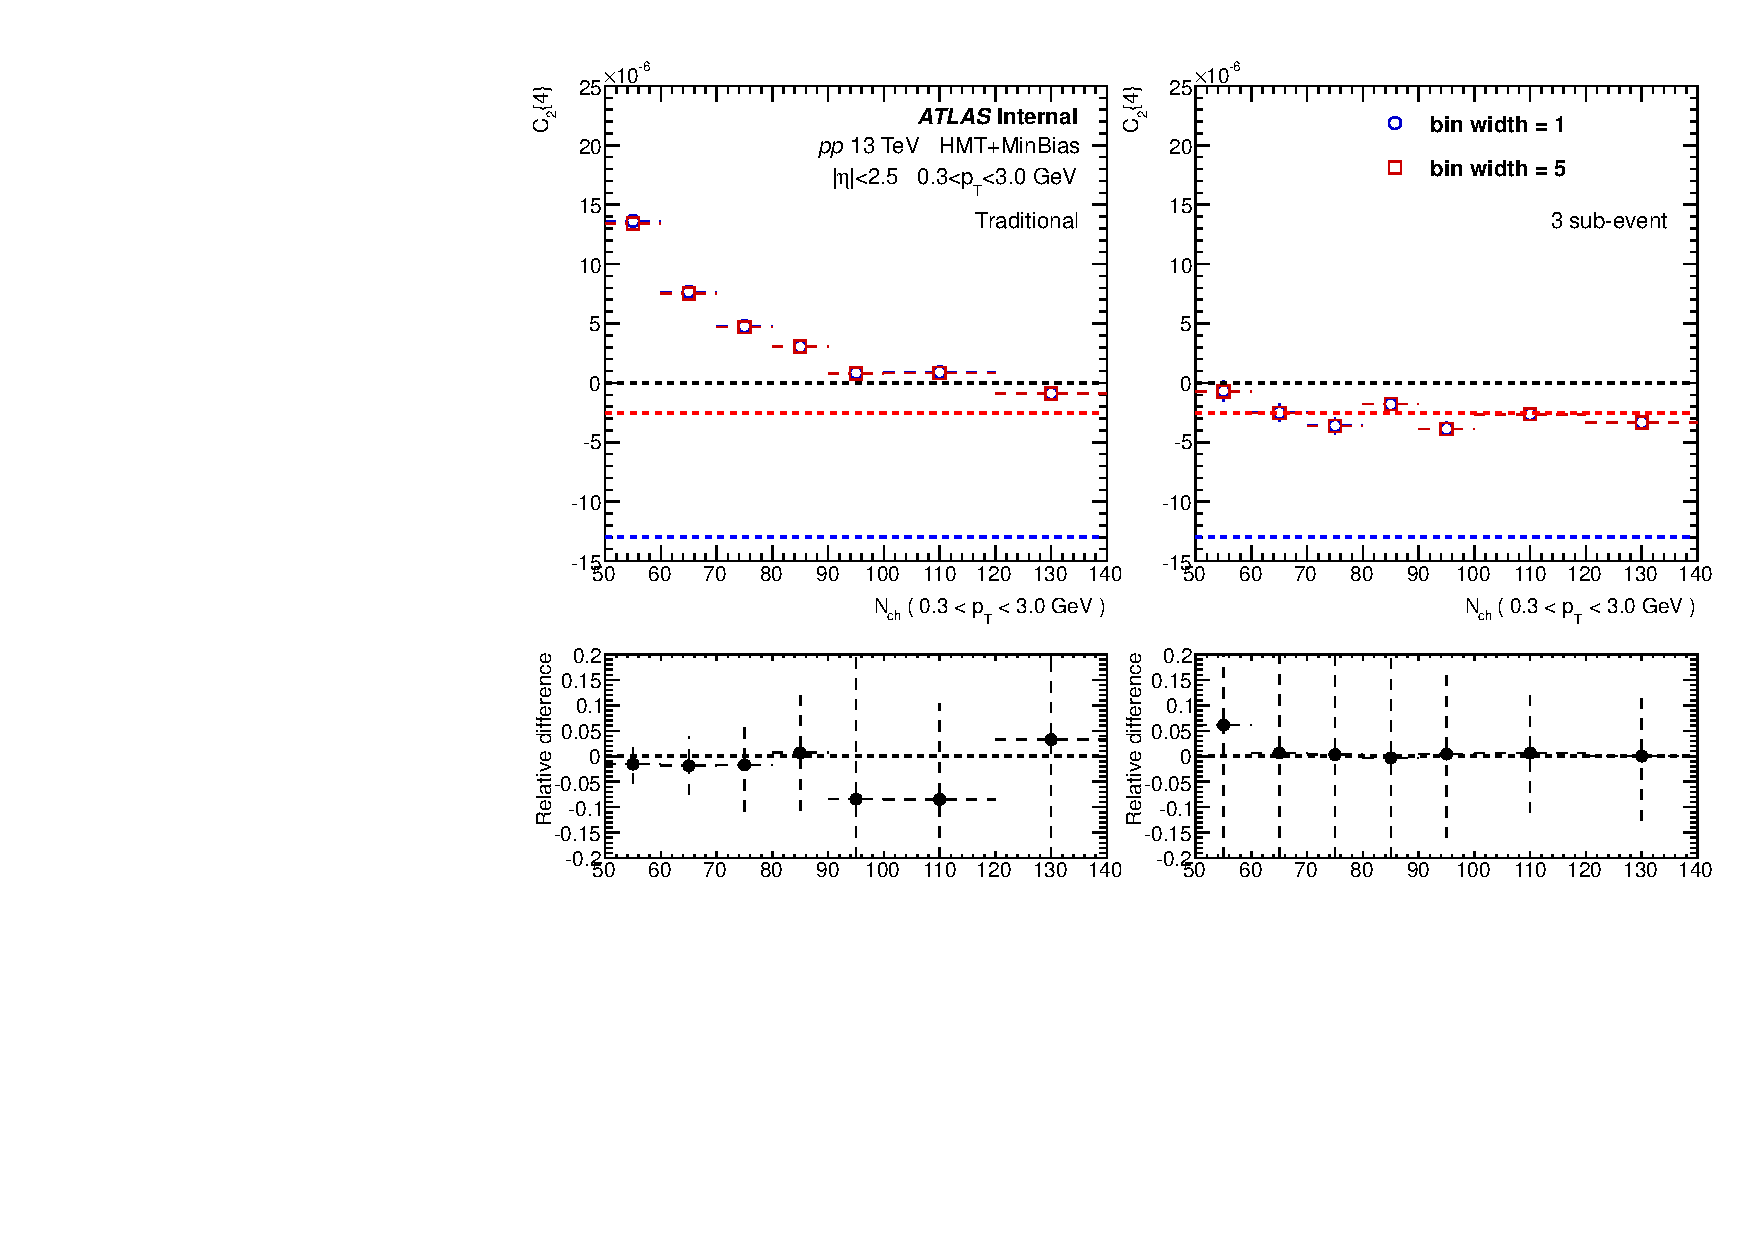
\includegraphics[width=0.8\linewidth]{figs/sec_sys/pp13/sys_pp13_binWidth1.pdf}
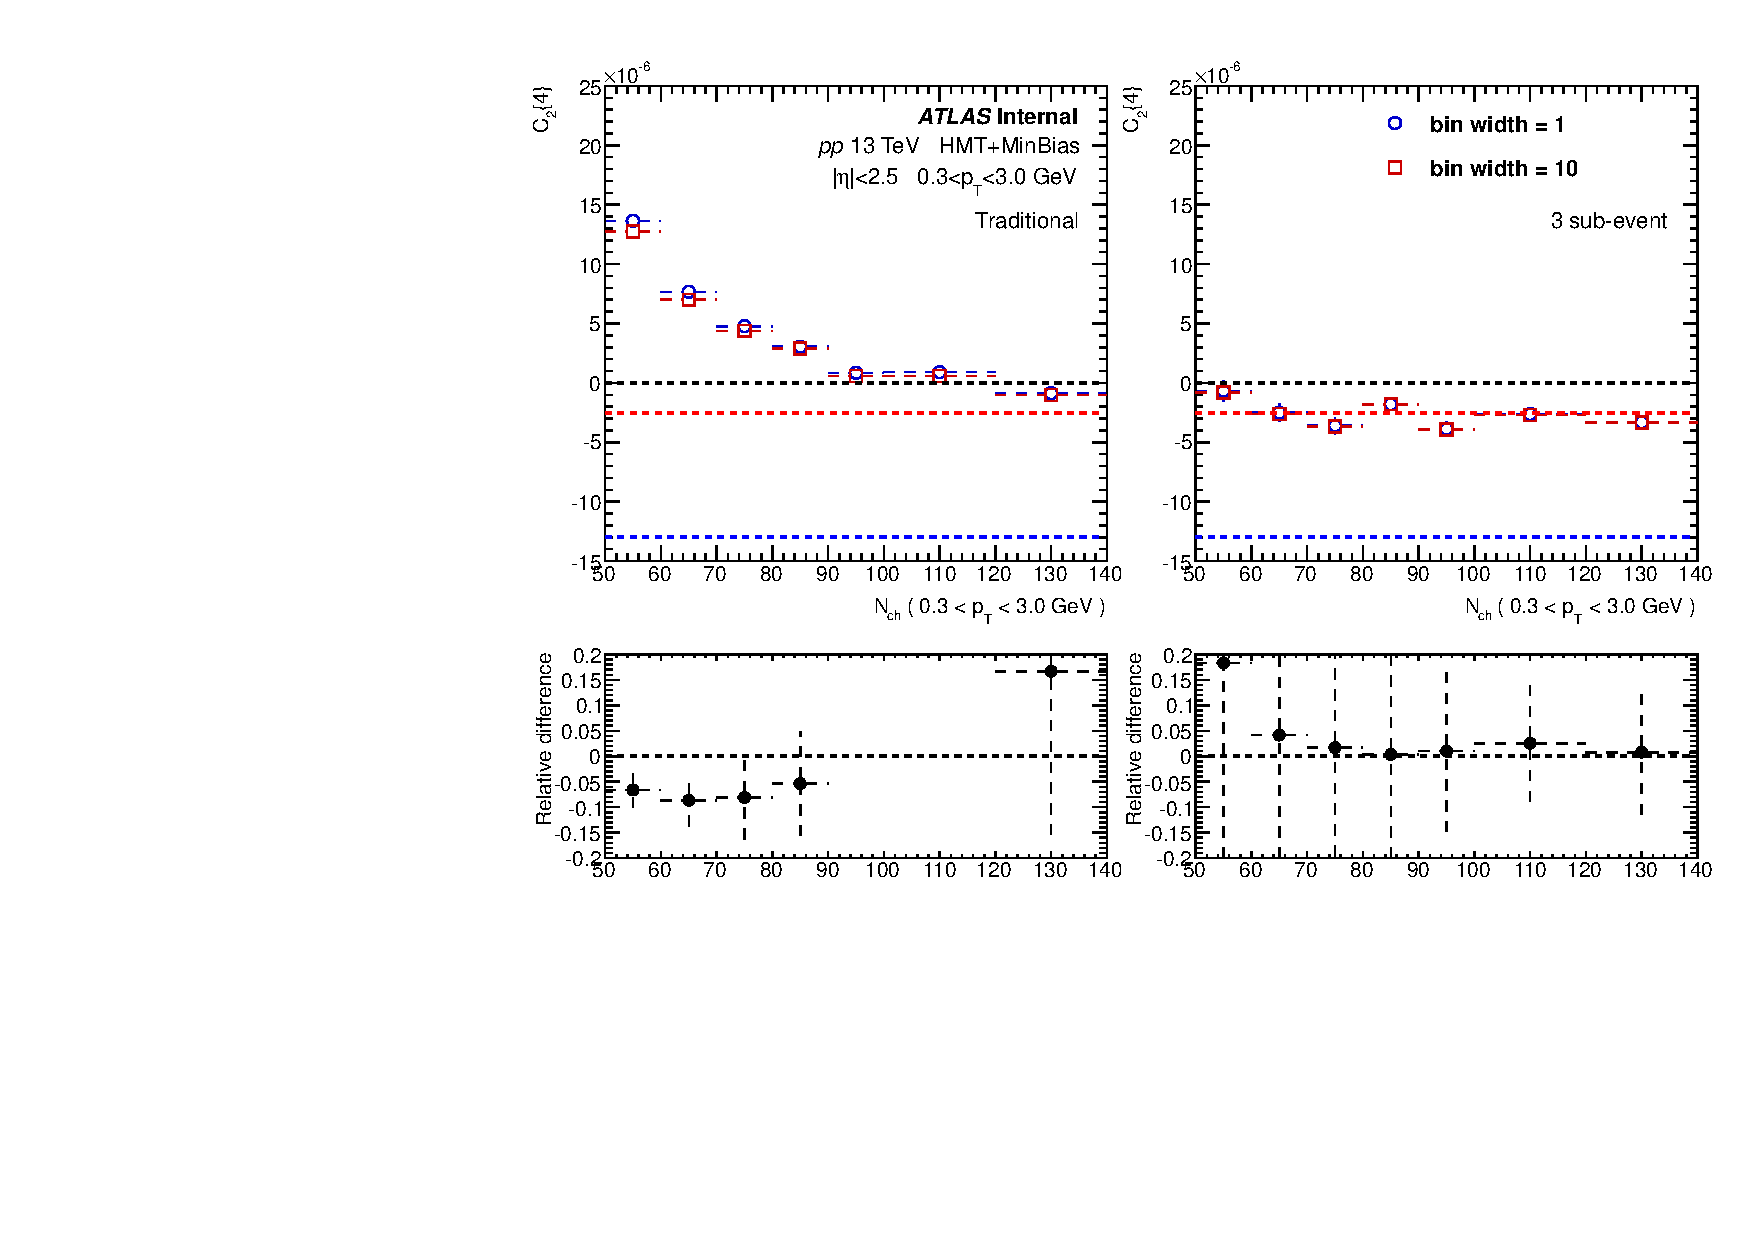
\includegraphics[width=0.8\linewidth]{figs/sec_sys/pp13/sys_pp13_binWidth2.pdf}
\caption{$C_{2}\{4\}$ measured with different event class bin widths. The left column has the results from traditional method and the right column from 3 sub-event method.}
\label{fig:sys_pp13_binWidth}
\end{figure}
If the bin width is increased from default 1 to 5 or even 10, the non-flow fluctuation in each event class could be different. Fig.~\ref{fig:sys_pp13_binWidth} compares the $C_{2}\{4\}$ with different bin widths. When event class bin width is increase to 5 tracks, $C_{2}\{4\}$ from traditional method slightly changes, within $5\%$. As a comparison, there is little change for $C_{2}\{4\}$ from the 3 sub-event method, the relative difference is minimal. This is even the case when the event class bin width is increased to 10 tracks: $C_{2}\{4\}$ from 3 sub-event method still has a relative difference within $5\%$, meanwhile the difference in traditional method is beyond $5\%$. This observation is exactly consistent with our expectation, since the 3 sub-event method further suppress the non-flow contribution and the additional multiplicity fluctuation due to the bin width changes does not cause any difference. We will come back to this point when we discuss the different event class definition based on $p_{T}$ of the particles. This check is only a cross-check to show the advantage of sub-event cumulant and will not be quoted as systematics.


\subsubsection{$\eta$ gap for sub-event}
Compared with 2 sub-event method, 3 sub-event method is designed mainly to remove the dijet-like correlation, since the chance that dijet still contribute to all the 3 sub-events are dramatically lowered compared with traditional cumulant. The only situation where dijet correlation still contributes to the 3 sub-event cumulant is when two jets from the dijet rest on the two boundaries of the 3 sub-events. In order to show whether the $C_{2}\{4\}$ is due to such little remaining dijet contributions, we introduced $\eta$ gaps between the sub-events to further suppress this contribution.

\begin{figure}[H]
\centering
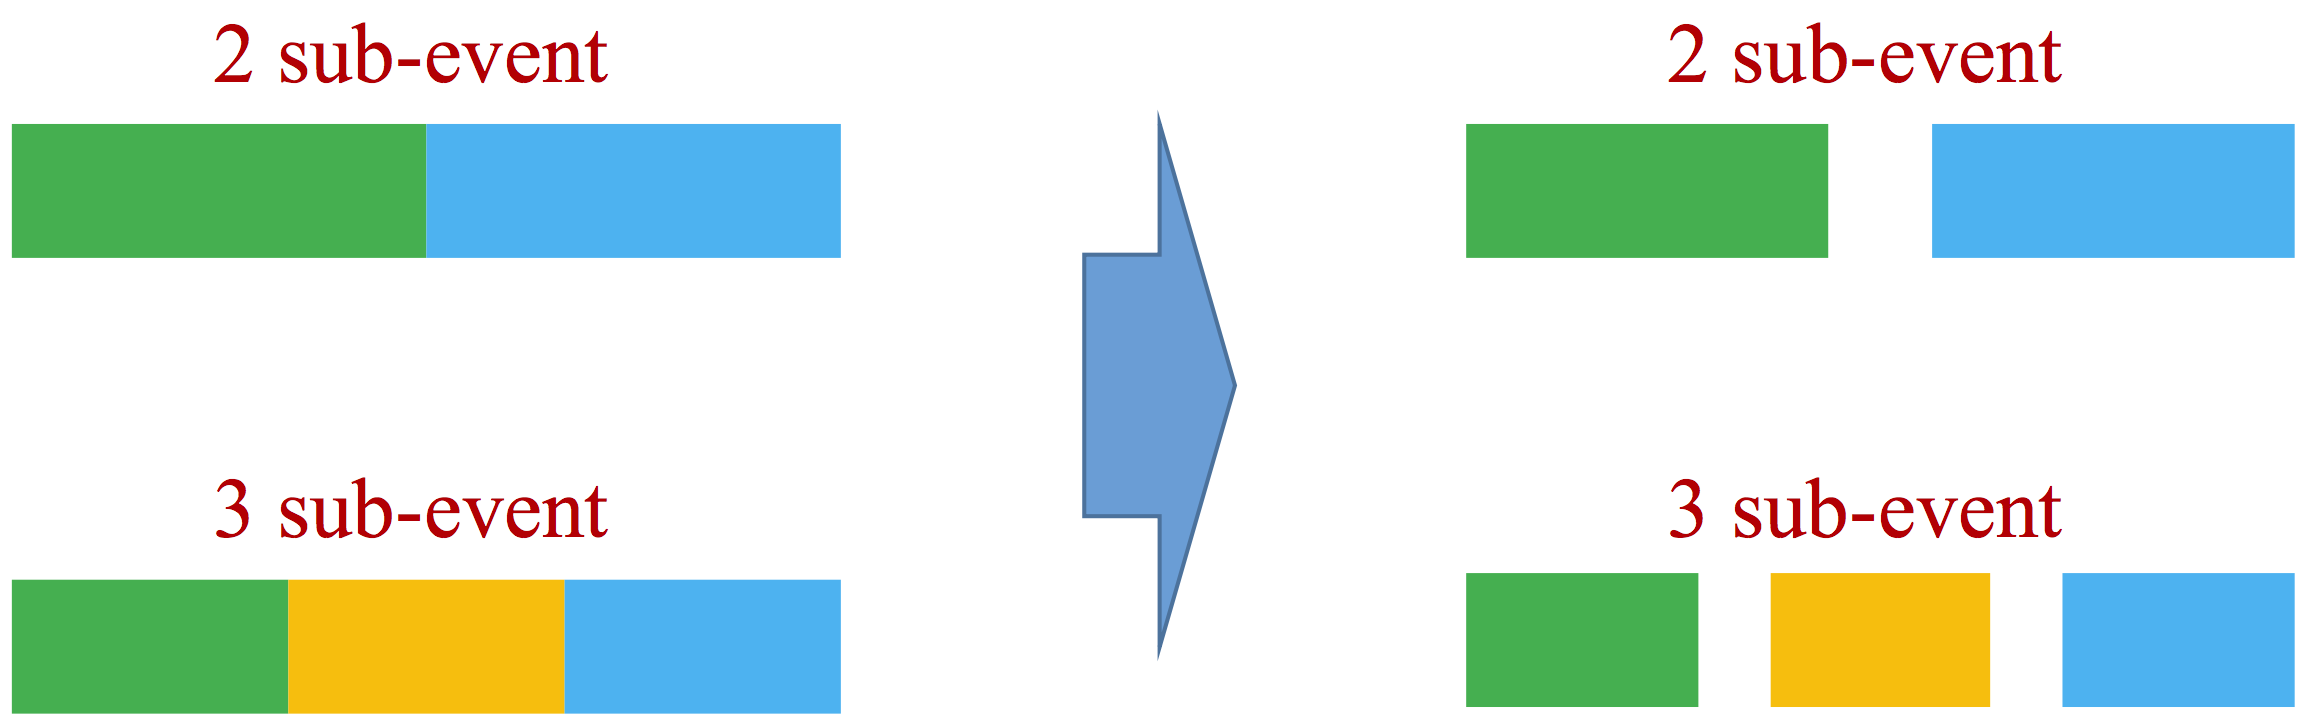
\includegraphics[width=0.8\linewidth]{figs/sec_sys/pp13/sys_pp13_gap_eg.png}
\caption{A cartoon showing the how the $\eta$ gaps are introduced to the 2 and 3 sub-event. The $\eta$ gap is $\Delta\eta=0.5$.}
\label{fig:sys_pp13_gap_eg}
\end{figure}
Fig.~\ref{fig:sys_pp13_gap_eg} describes the basic idea of the $\eta$ gap between the sub-events: in the 2 sub-event case, we introduced a $\eta$ gap with $\Delta\eta=0.5$ between 2 sub-events and in the 3 sub-event case, two $\eta$ gaps with $\Delta\eta=0.5$ have been added among three sub-events. The advantage of add $\eta$ gaps is removing the residual dijet correlation and the drawback is reducing the number of particle pairs, especially in 4-particle cumulant. Thus the purpose of this check is estimating the contributing of remaining non-flow, the default method is still without $\eta$ gap, to gain better statistical significance.

\begin{figure}[H]
\centering
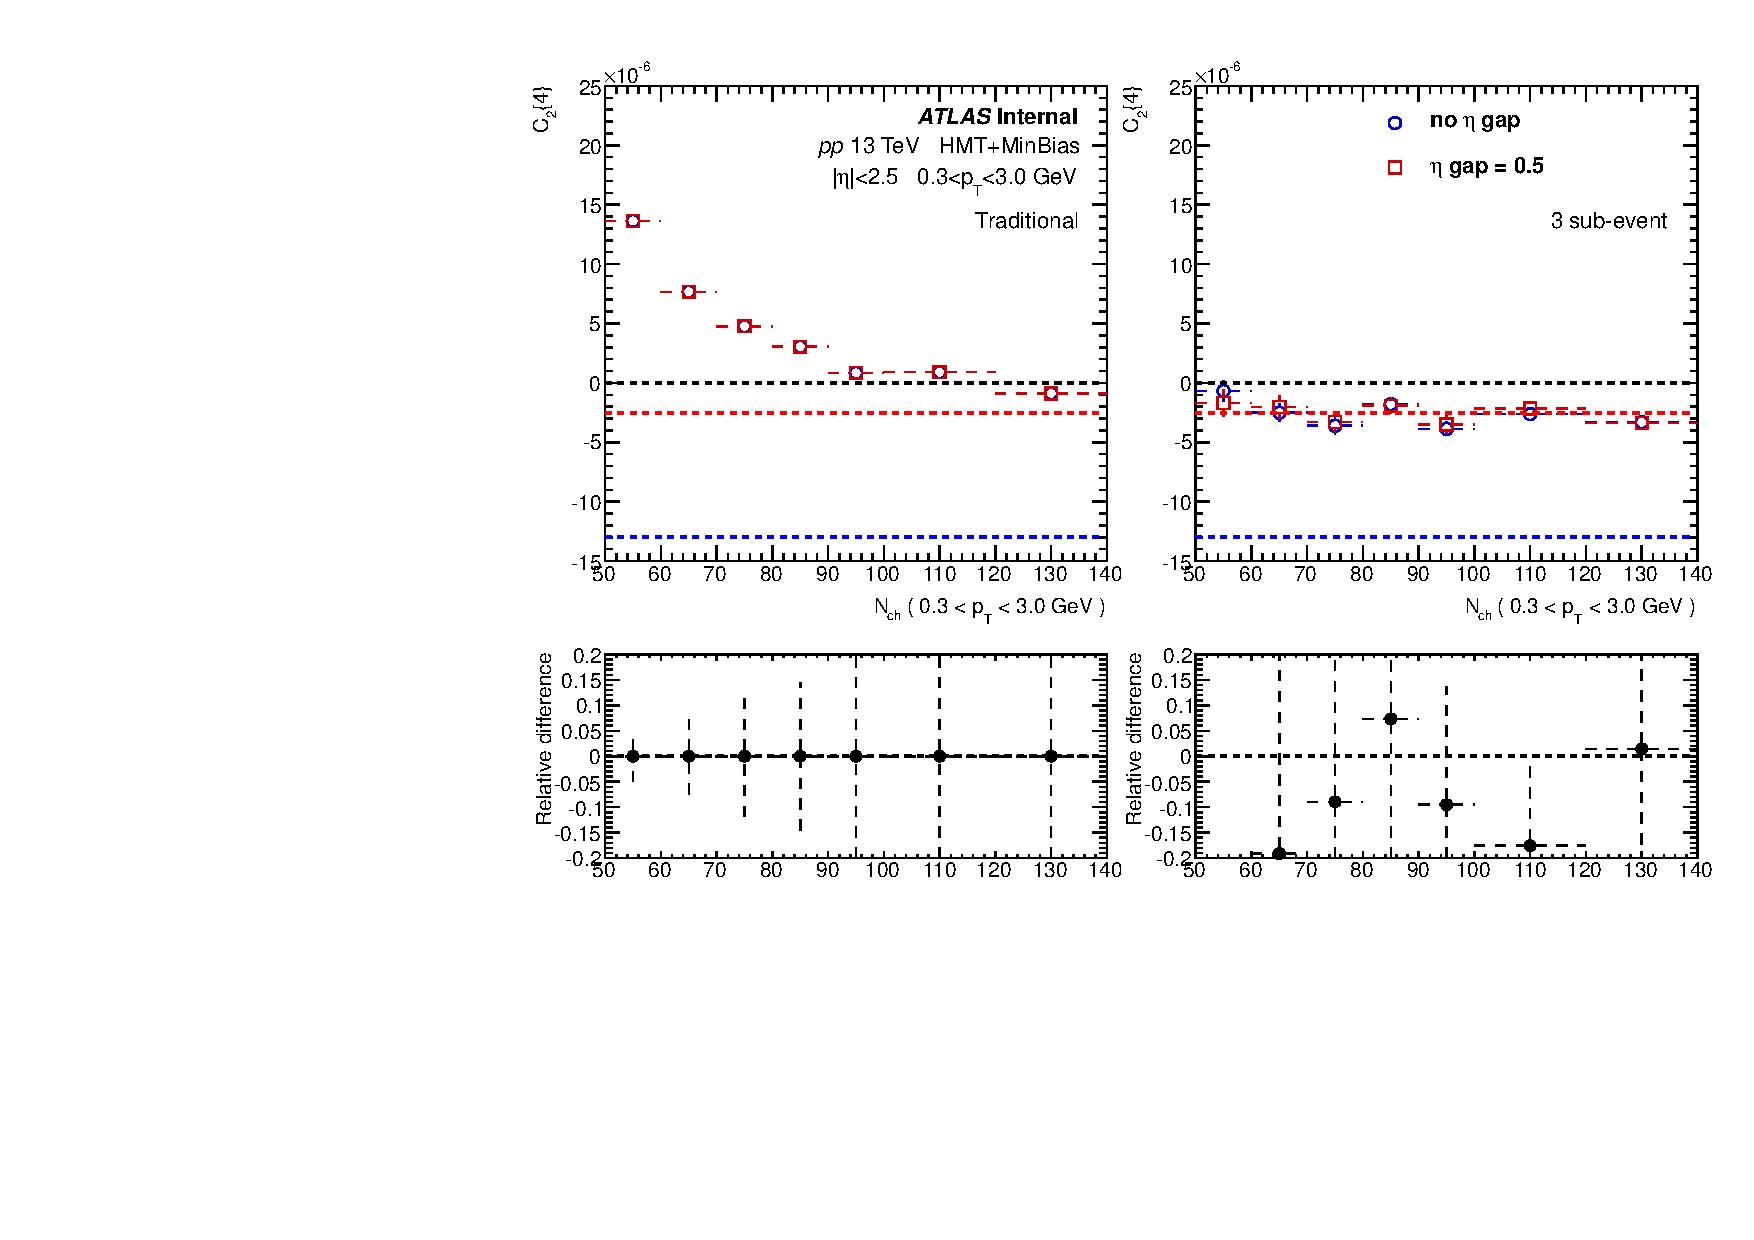
\includegraphics[width=0.8\linewidth]{figs/sec_sys/pp13/sys_pp13_gap.pdf}
\caption{$C_{2}\{4\}$ measured with and without $\eta$ gaps between sub-events. The left column has the results from traditional method and the right column from 3 sub-event method.}
\label{fig:sys_pp13_gap}
\end{figure}
Fig.~\ref{fig:sys_pp13_gap} shows the $C_{2}\{4\}$ measured with and without $\eta$ gaps between sub-events. Since there is no $\eta$ gap introduced for traditional cumulant, the relative difference is 0 by construction. For 3 sub-event method, with $\eta$ gap does not change the observation: even though the relative difference is fluctuating around 0 on the level of more than $10\%$, but that is partially due to the larger statistical errors with presence of $\eta$ gap. Due to these reasons, the default case is without $\eta$ gap and this check will not be quoted as systematics.



\subsubsection{Charge dependence}
Since most short-range non-flow correlations are originated from decay and jets, they are supposed to be stronger in the opposite charge combination than same charge. Subevent method provides a natural way to test this charge dependence.

\begin{figure}[H]
\centering
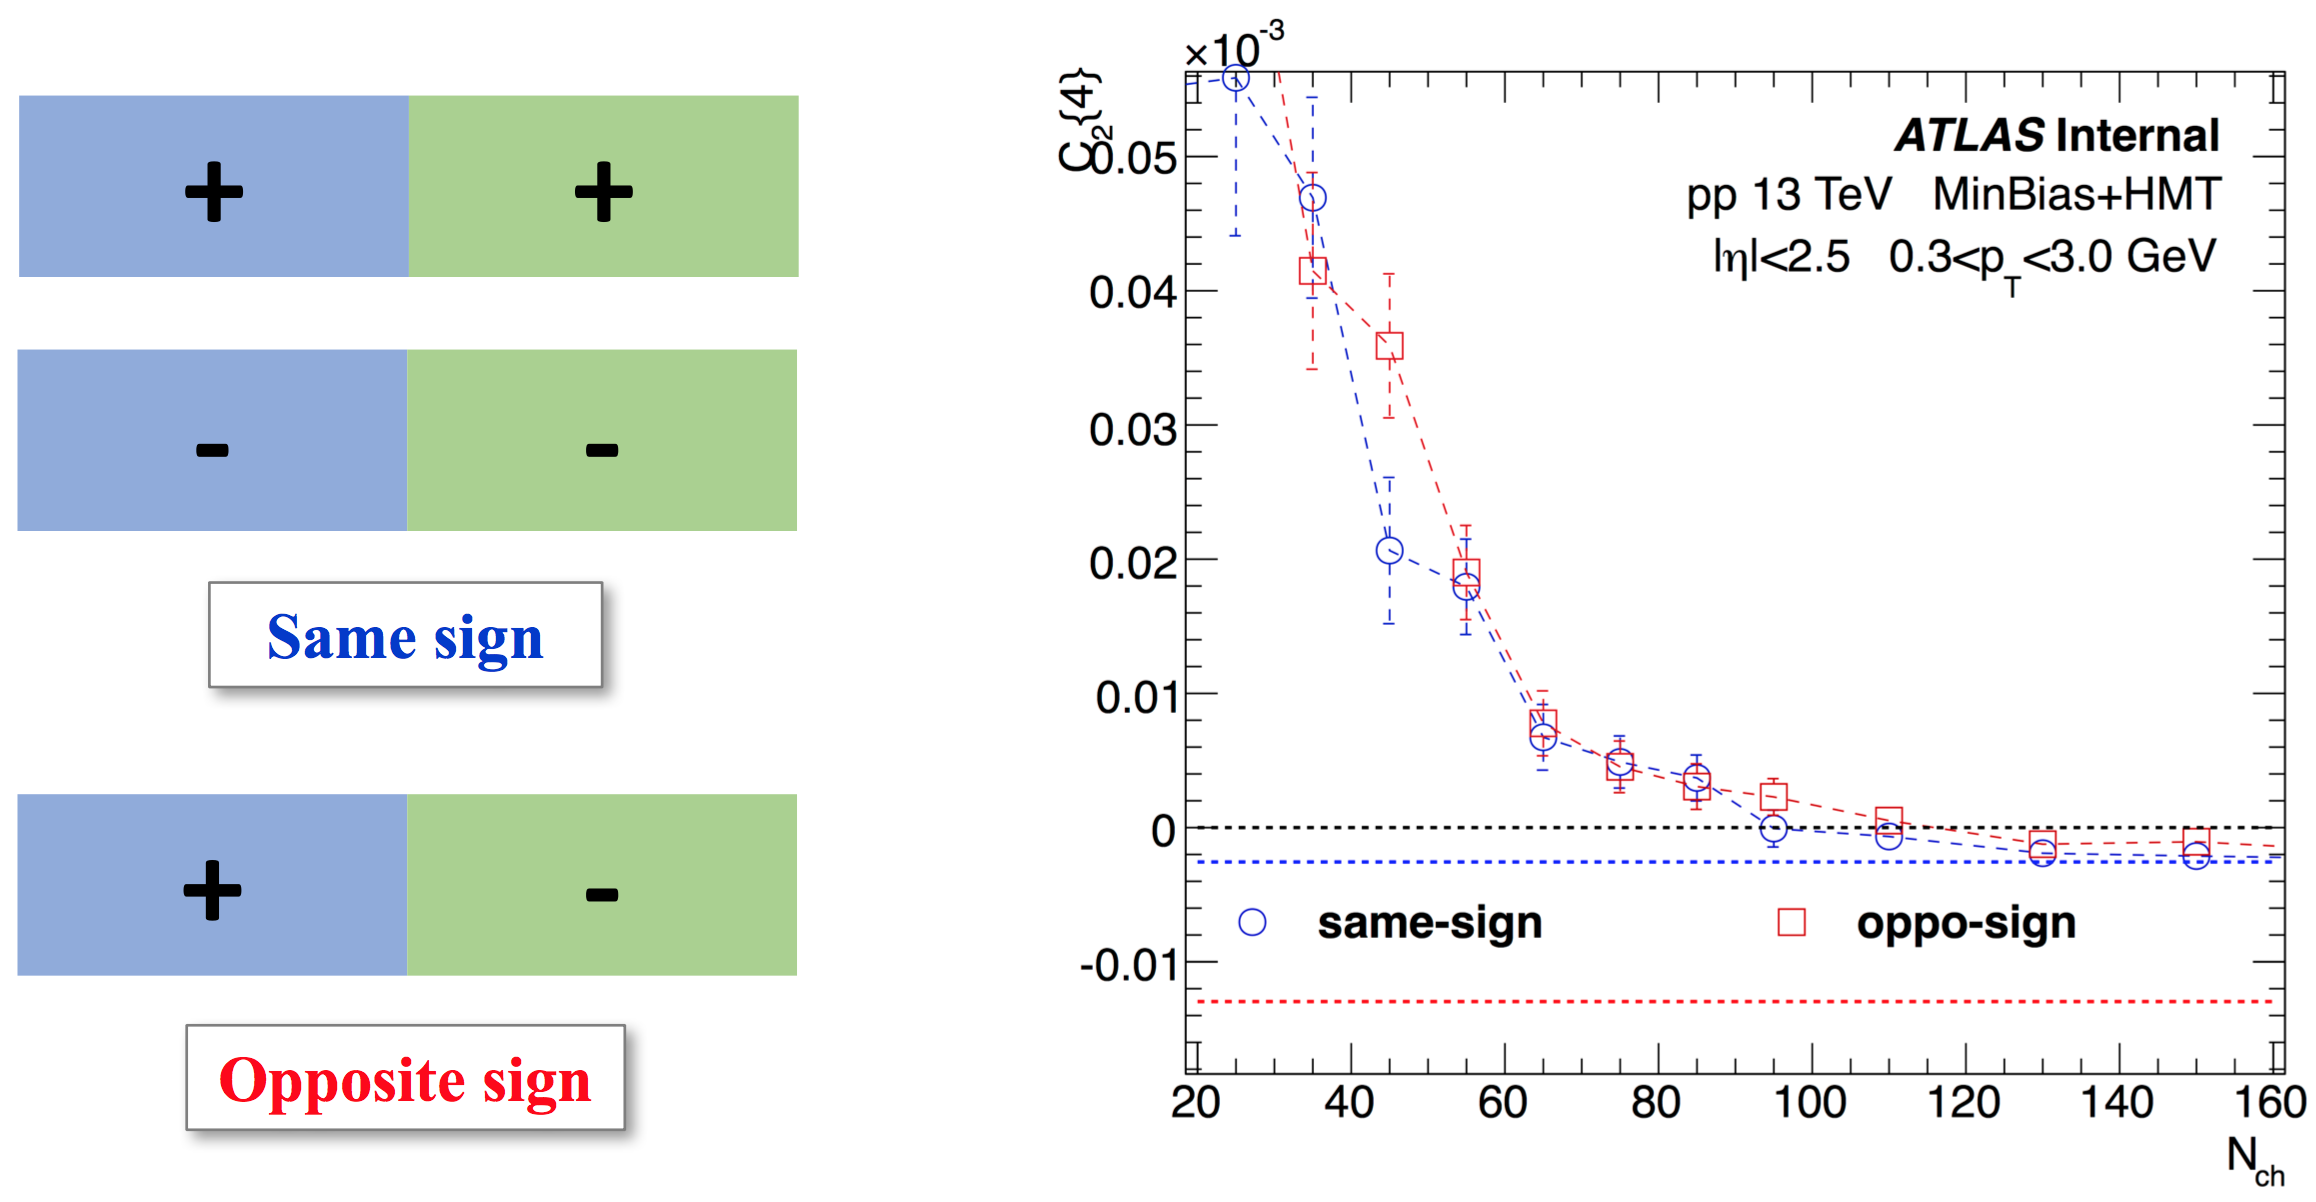
\includegraphics[width=0.8\linewidth]{figs/sec_sys/pp13/charge_dependence_2sub.png}
\caption{Left plot shows the configuration for same and opposite change in 2 subevent cumulant. Right plot show the comparison of $c_{2}\{4\}$ measured using only same change and opposite charge. The blue and red dash line indicate the $4\%$ and $6\%$ flow respectively.}
\label{fig:charge_dependence_2sub}
\end{figure}
The configurations of same-sign and opposite-sign are shown in the left plot in Fig.~\ref{fig:charge_dependence_2sub}, where same-sign combination has both $++$ and $--$ charges in the 2 subevents, while one $+$ and one $-$ charges in 2 subevents for the opposite-sign. The comparison of $c_{2}\{4\}$ measured in these two configurations are shown in the right plot. $c_{2}\{4\}$ from opposite sign is slightly larger than the same sign, which is expected since the majority of short-range non-flow are suppressed in the 2 subevent cumulant.



\subsubsection{Deviations from the truth in the reconstruction of Monte Carlo data}
The PYTHIA 8 Monte Carlo simulations were used to evaluate the difference between 4-particle cumulants in $pp$ data calculated using the generated and reconstructed charged particles obtained using the same analysis method. In some analysis it is considered as a crosscheck, since it assesses the quality of tracking, which are separately accounted for in previous systematics. The argument for not accounting it as a systematic uncertainties also relies on the fact that MC generators do not properly describe the investigated particle correlations. Nevertheless, we think that it still be considered as a validation of the analysis method, even though PYTHIA does not include any flow effect. This is only a cross-check, and will not be included as the systematics.

\begin{figure}[H]
\centering
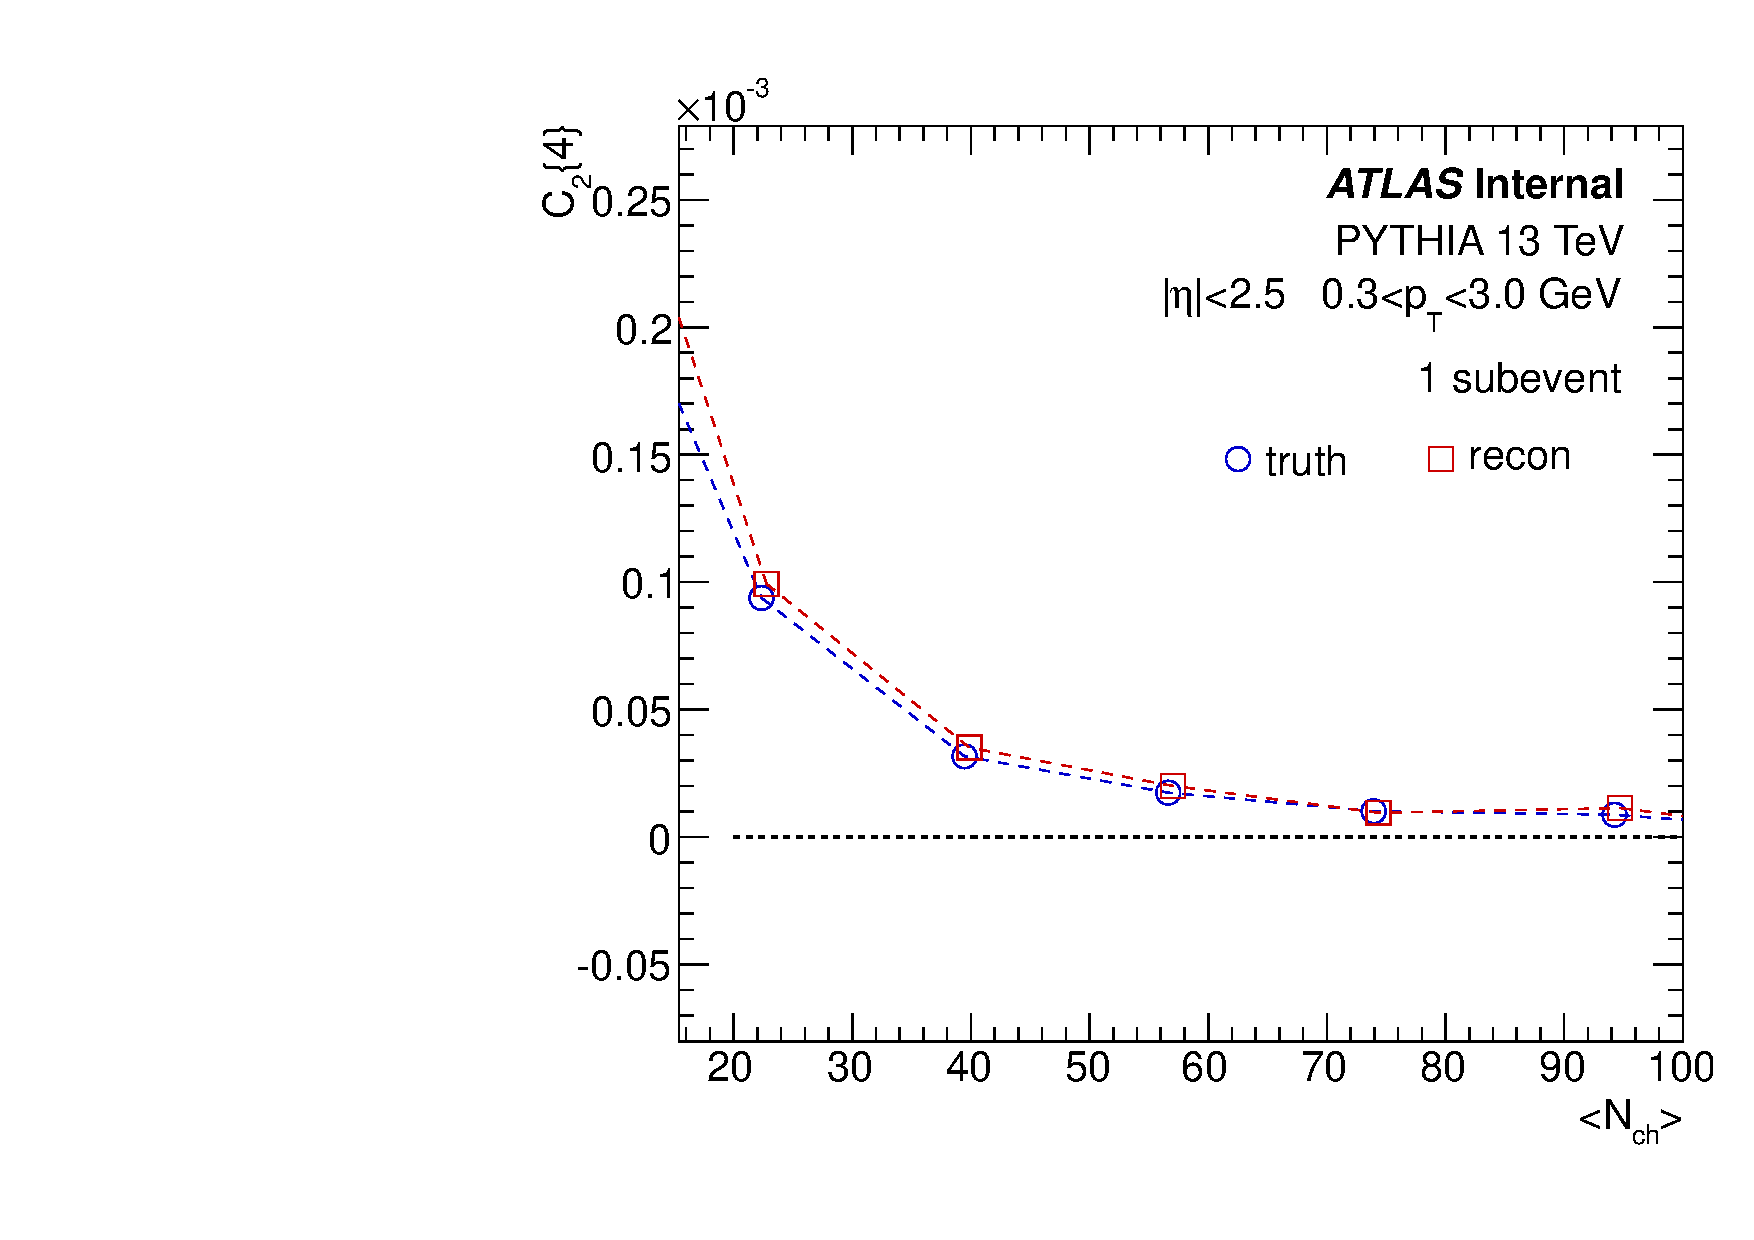
\includegraphics[width=0.45\linewidth]{figs/sec_sys/pp13/MC_closure_1sub_pt0.pdf}
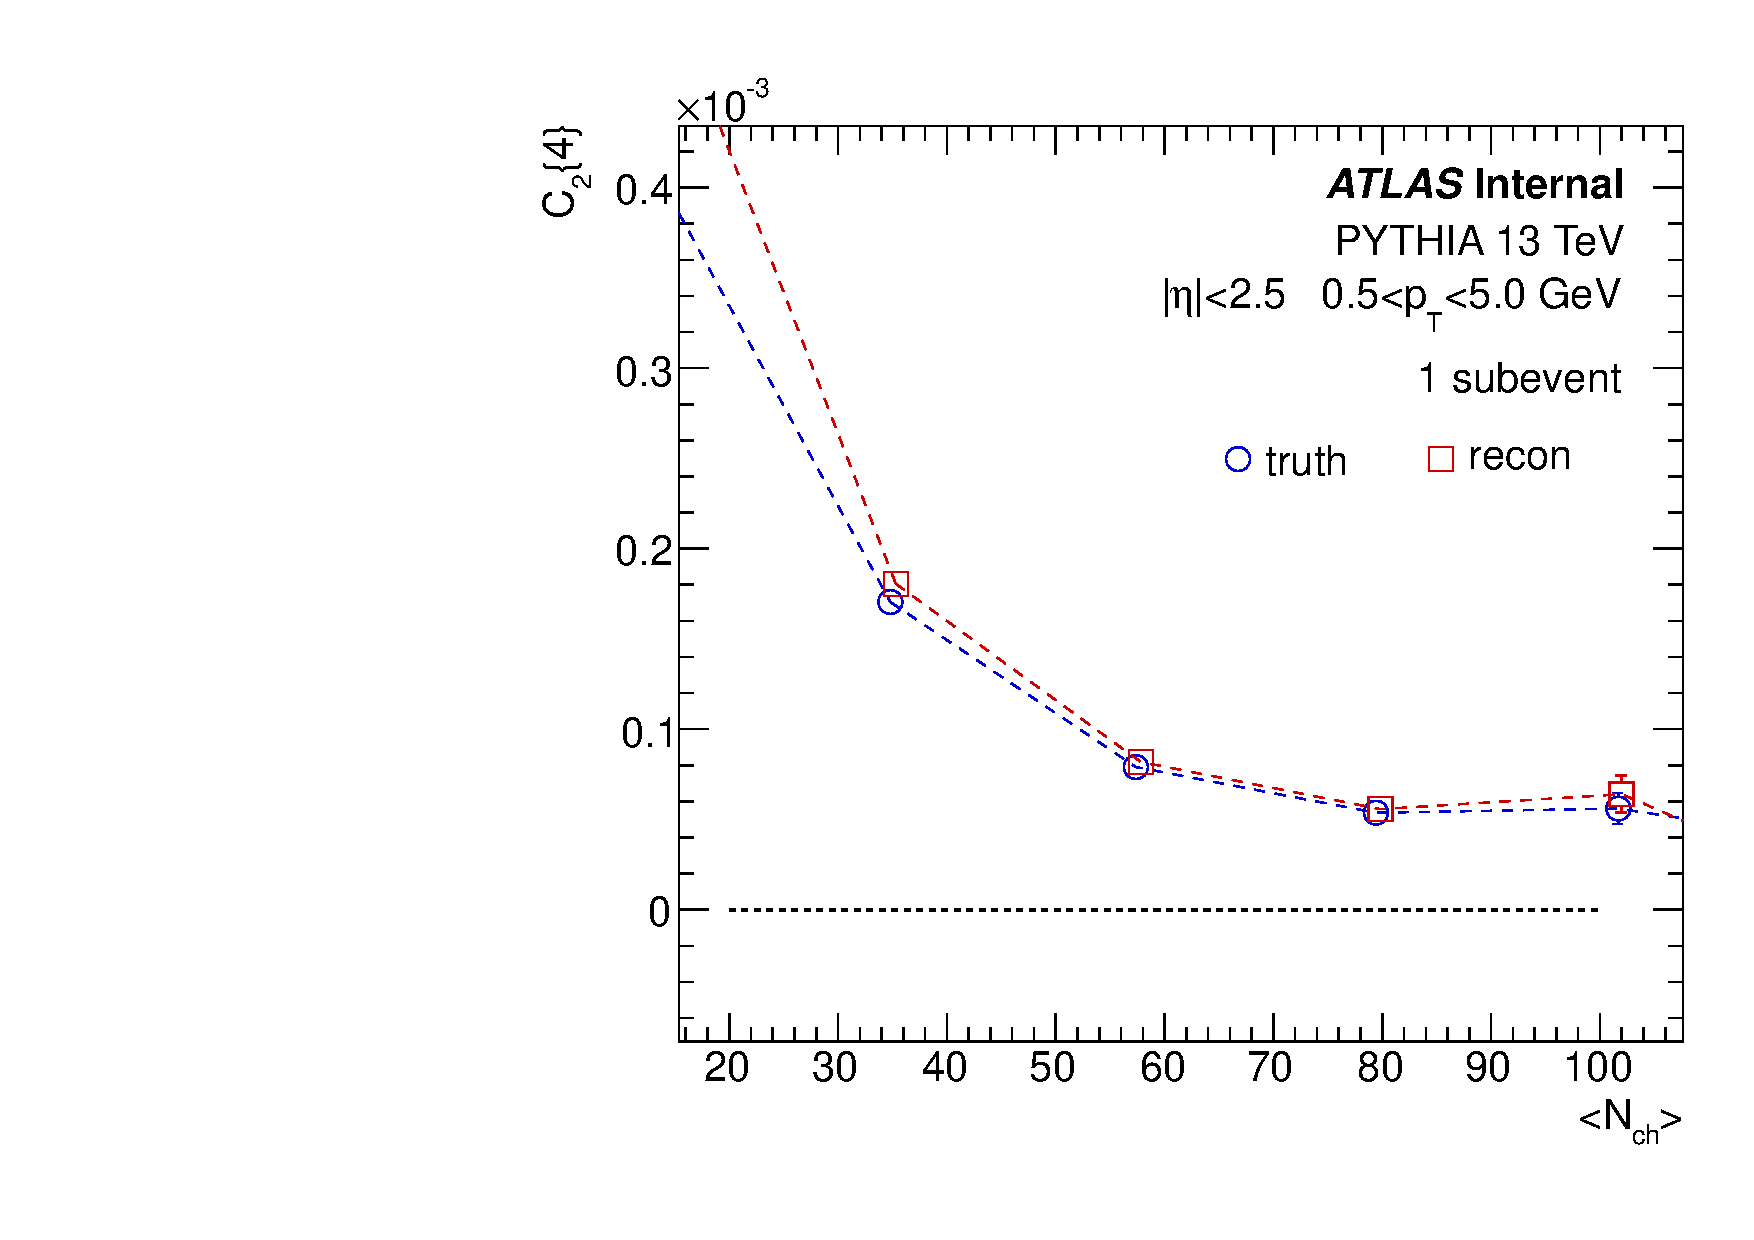
\includegraphics[width=0.45\linewidth]{figs/sec_sys/pp13/MC_closure_1sub_pt1.pdf}
\caption{Comparison of the 4-particle cumulants $c_{2}\{4\}$ for 13 TeV PYTHIA, calculated with the reconstructed and generated charged particle for $0.3<p_{\text{T}}<3.0$ GeV (left) and $0.5<p_{\text{T}}<5.0$ GeV (right). The cumulant is calculated using the standard method (1 subevent).}
\label{fig:MC_closure_1sub}
\end{figure}

Fig.~\ref{fig:MC_closure_1sub} illustrates the evaluation of the MC closure test for $pp$, for $0.3<p_{\text{T}}<3.0$ GeV (left) and $0.5<p_{\text{T}}<5.0$ GeV (right). For the standard cumulant, $c_{2}\{4\}$ from reconstructed tracks is slightly larger than the $c_{2}\{4\}$ from truth particles. The small difference could be due to several reasons: 1) tracking efficiency is slightly dependent of $N_{\text{ch}}$, which has not been taken into account when applying the efficiency; 2) even though events are binned based on the corrected number of charged particles, in each event class, the events from truth and reconstructed are not identical due to event-by-event fluctuations, which might have an impact on the 4-particle cumulant $c_{2}\{4\}$; 3) tracking efficiency does not take non-uniformness in $\phi$ into account, which could also result in small differences.

\begin{figure}[H]
\centering
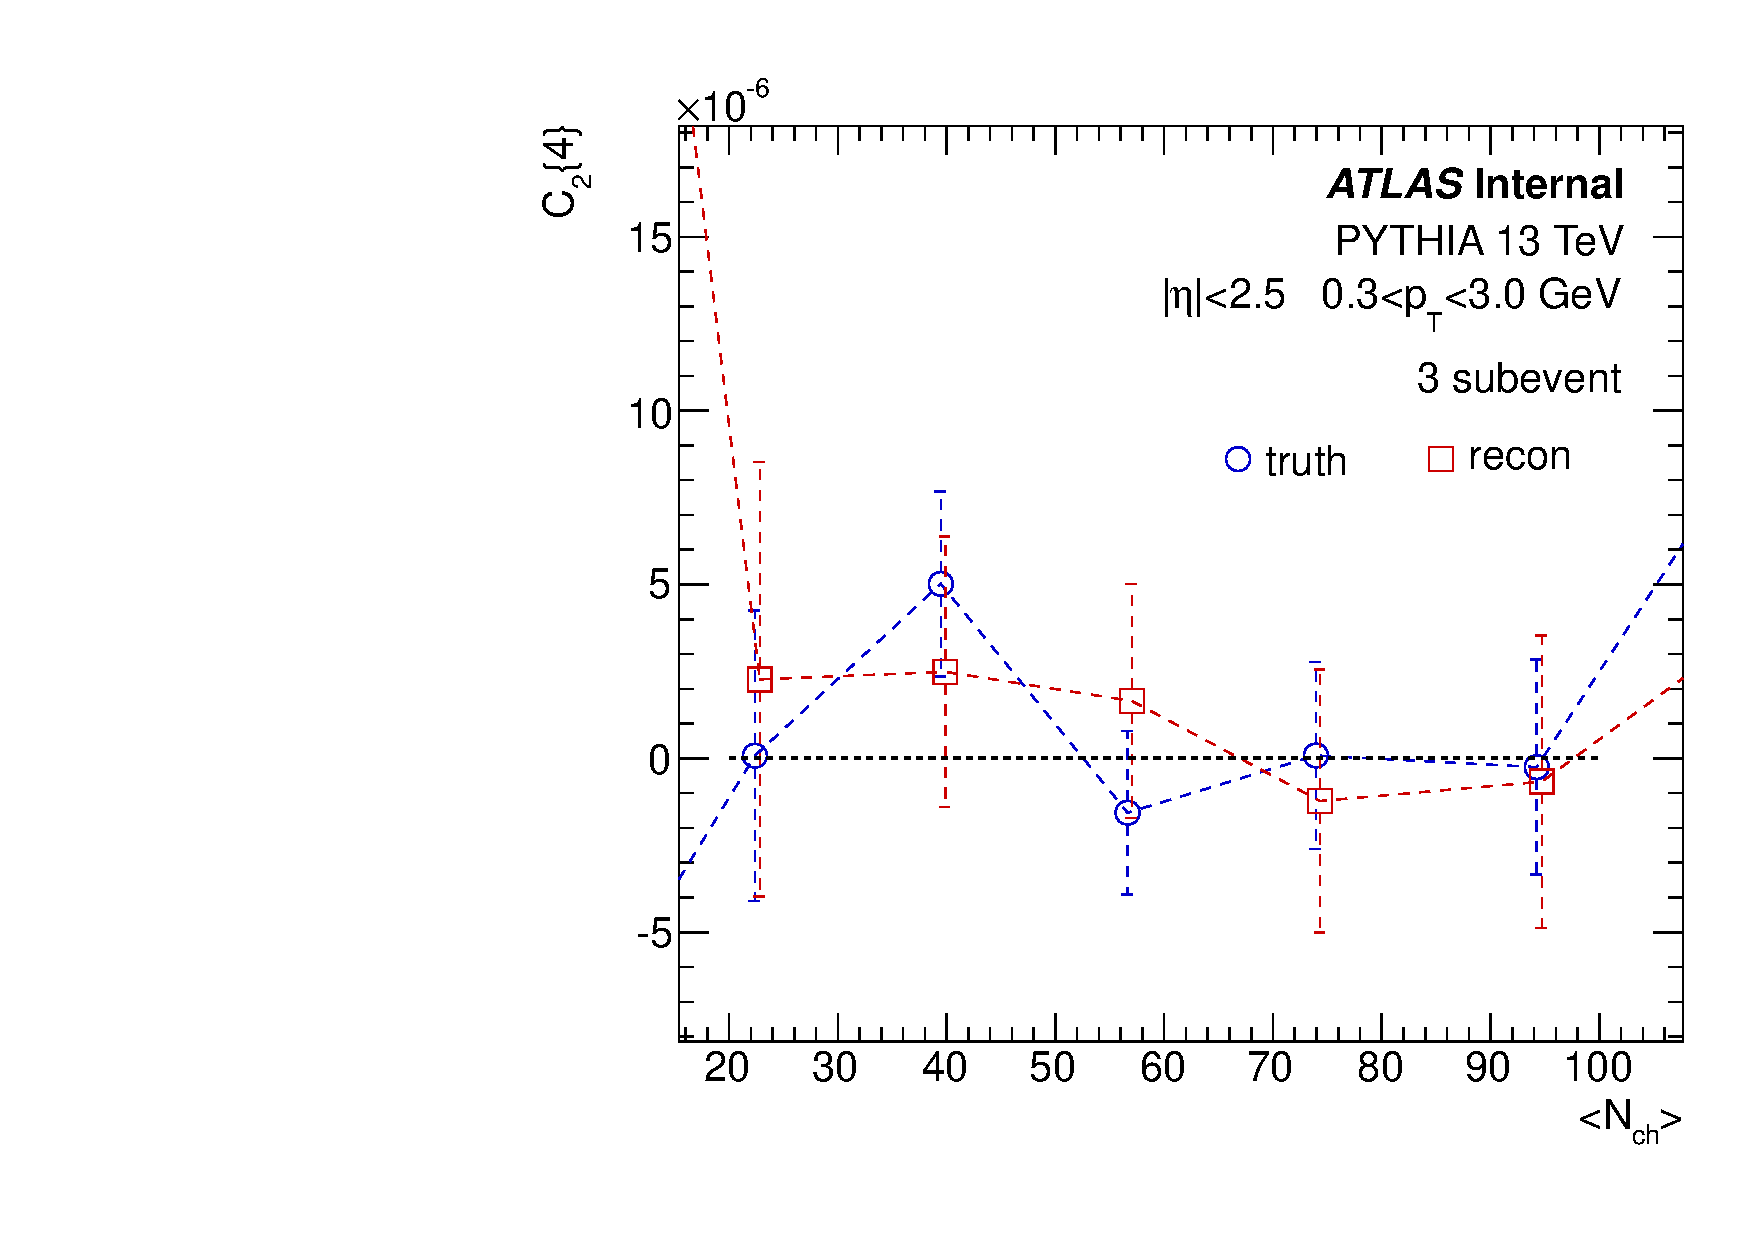
\includegraphics[width=0.45\linewidth]{figs/sec_sys/pp13/MC_closure_3sub_pt0.pdf}
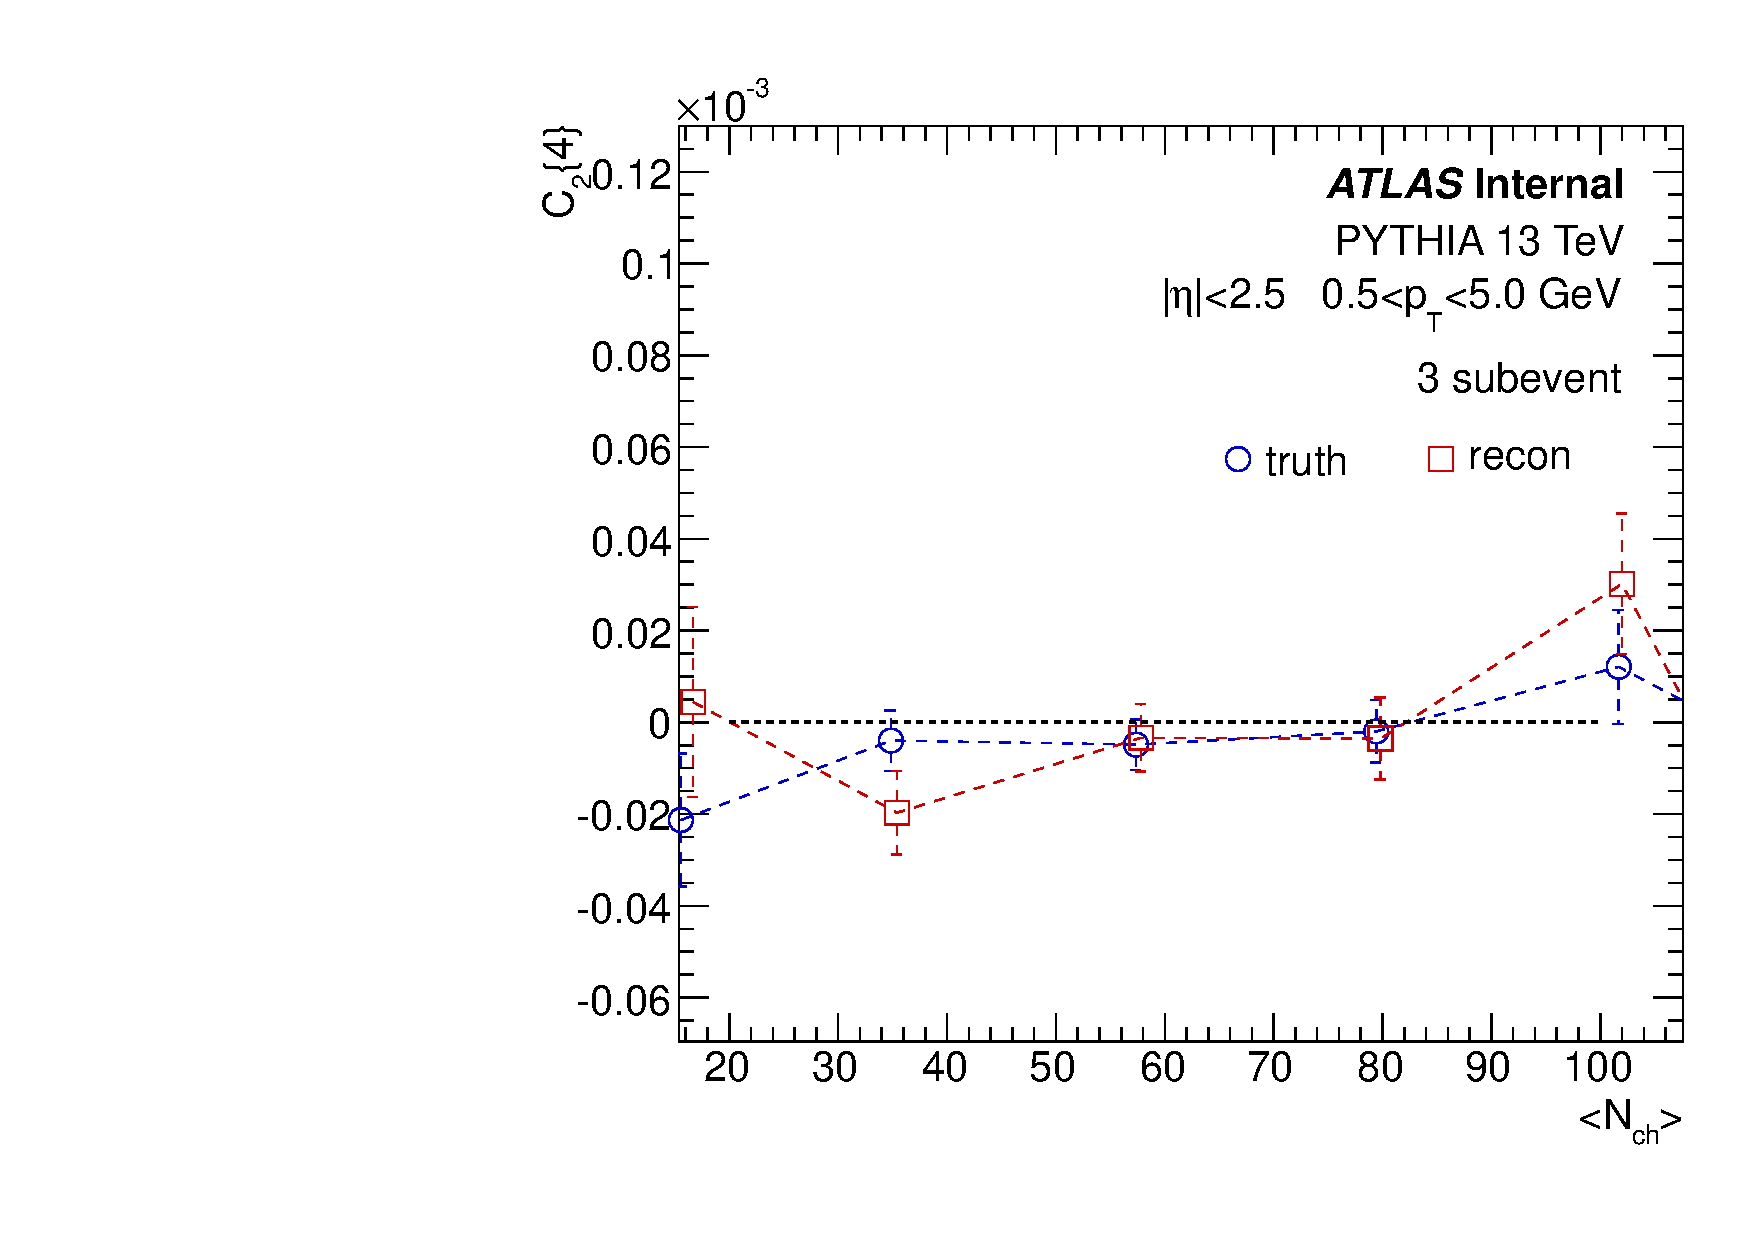
\includegraphics[width=0.45\linewidth]{figs/sec_sys/pp13/MC_closure_3sub_pt1.pdf}
\caption{Comparison of the 4-particle cumulants $c_{2}\{4\}$ for 13 TeV PYTHIA, calculated with the reconstructed and generated charged particle for $0.3<p_{\text{T}}<3.0$ GeV (left) and $0.5<p_{\text{T}}<5.0$ GeV (right). The cumulant is calculated using 3 subevent method.}
\label{fig:MC_closure_3sub}
\end{figure}

As a comparison, Fig.~\ref{fig:MC_closure_3sub} shows the same check but calculated with 3 subevent method. With current statistics, the difference of $c_{2}\{4\}$ between truth and reconstructed seems to be smaller than standard method, and both of them fluctuates around 0. Since PYTHIA does not include any flow effect, this plot supports that 3 subevent method can effectively suppress the non-flow: $c_{2}\{4\}$ is much closer to 0 compared with standard method. Furthermore, the smaller difference between truth and reconstructed could also indicate that the second reason listed above could be the reason why in standard cumulant $c_{2}\{4\}$ from reconstructed tracks is slightly higher than the $c_{2}\{4\}$ from truth particles: additional event-by-event non-flow fluctuation can cause the difference. While with 3 subevent method, since the non-flow is suppressed, the difference is much smaller.

\begin{figure}[H]
\centering
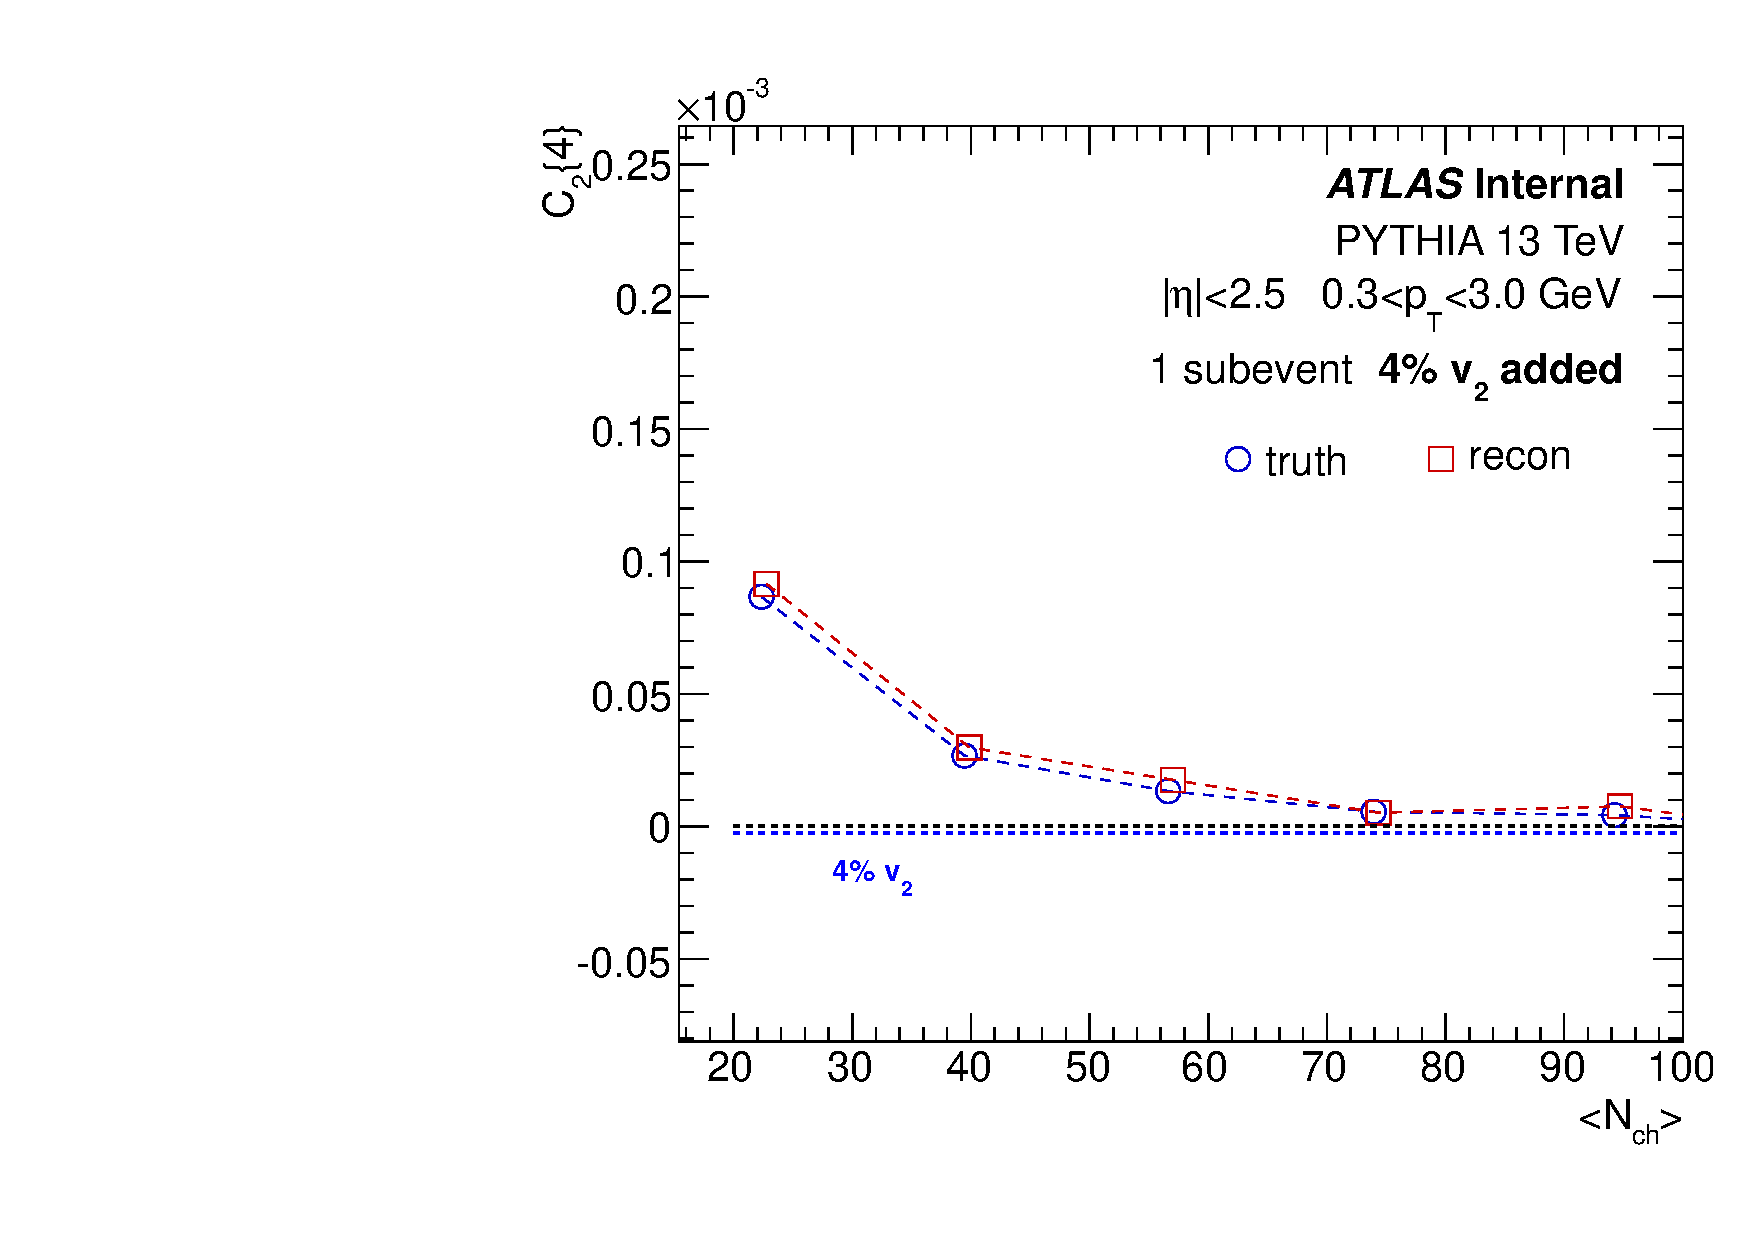
\includegraphics[width=0.45\linewidth]{figs/sec_sys/pp13/MC_closure_1sub_flow.pdf}
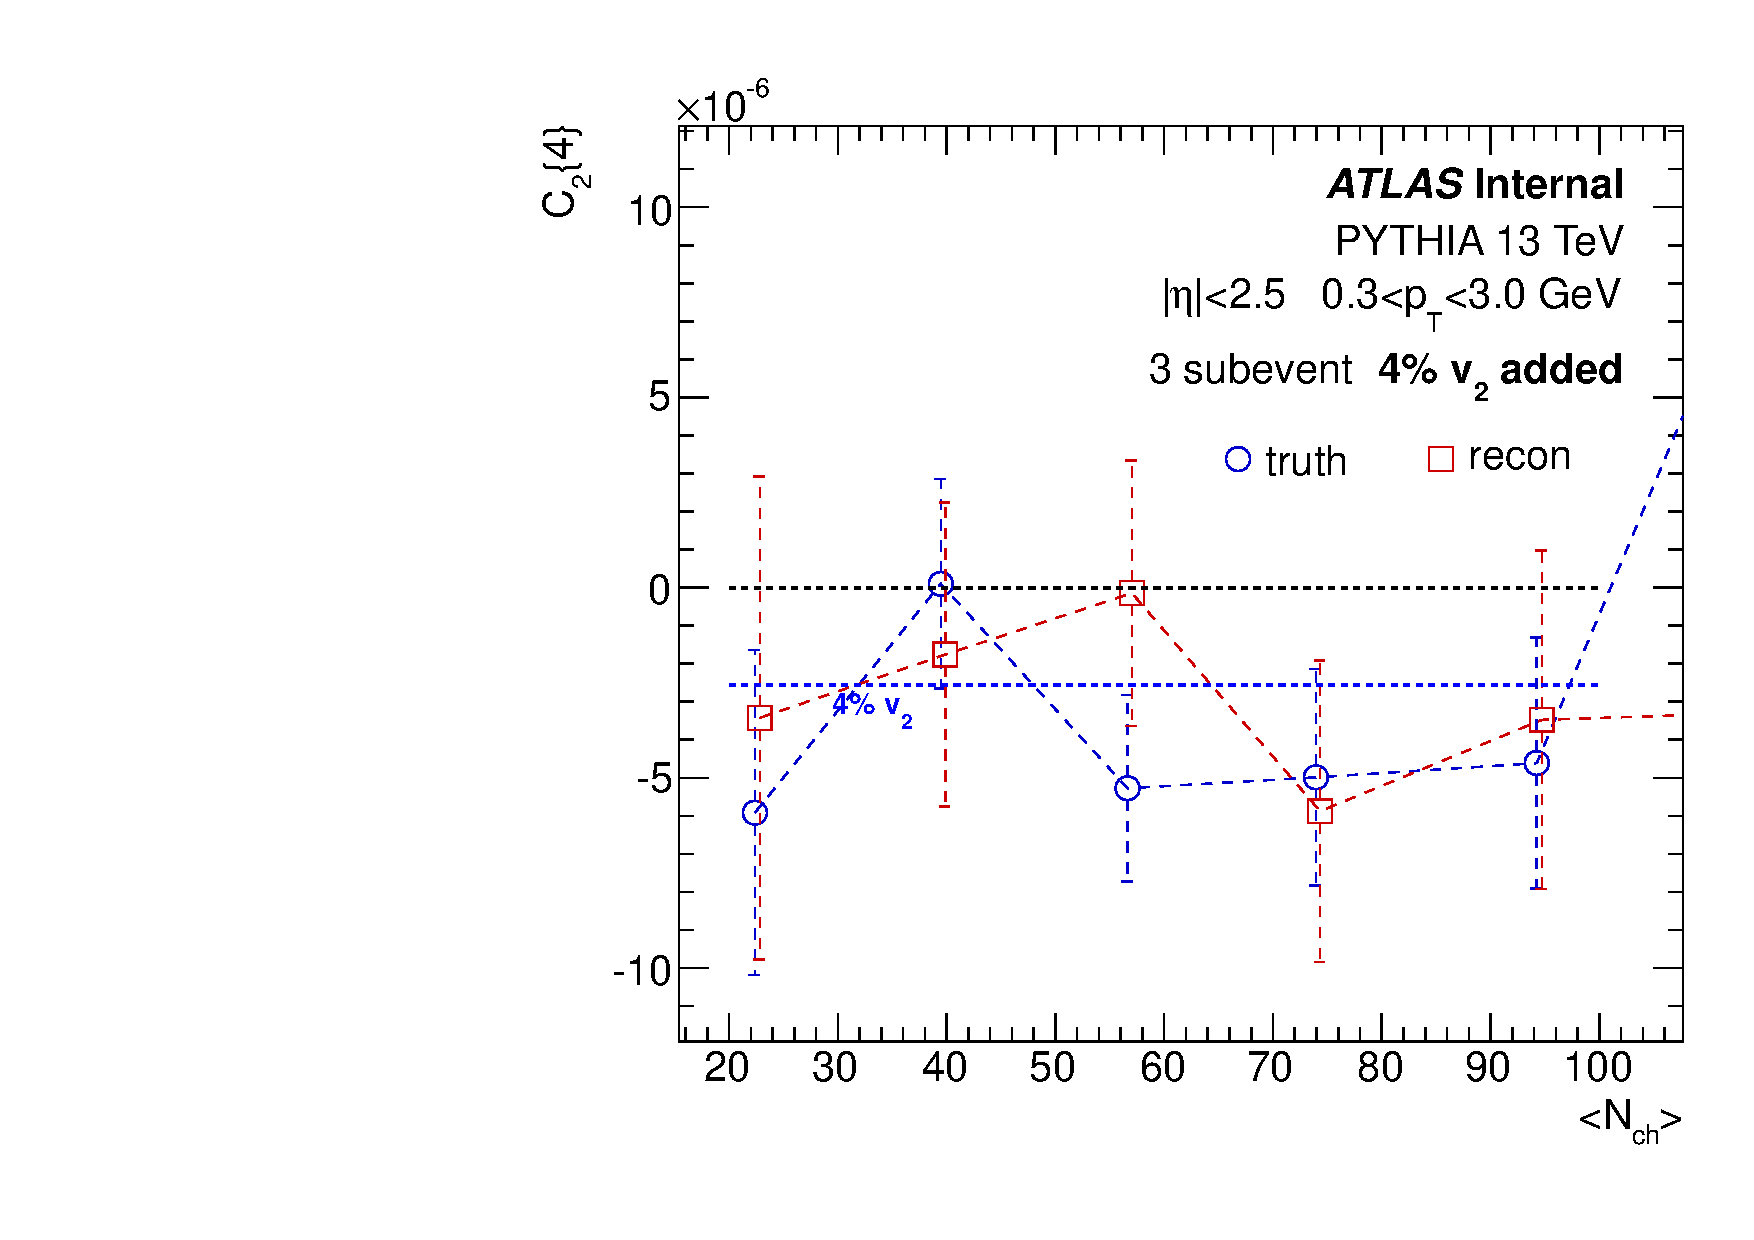
\includegraphics[width=0.45\linewidth]{figs/sec_sys/pp13/MC_closure_3sub_flow.pdf}
\caption{Comparison of the 4-particle cumulants $c_{2}\{4\}$ for 13 TeV PYTHIA, calculated with the reconstructed and generated charged particle for $0.3<p_{\text{T}}<3.0$ GeV, with $4\%$ $v_{2}$ imposed to the generated and reconstructed events (indicated by the blue dash line). The left plot is calculated using standard method and the right plot using 3 subevent method.}
\label{fig:MC_closure_flow}
\end{figure}
To quantify the performance of the three methods for recovering the underlying flow signal, a flow afterburner is used to add a constant $v_{2}$ to the generated and reconstructed PYTHIA events. Fig.~\ref{fig:closure_flow} shows the calculated $c_{2}\{4\}$ with $4\%$ imposed to the generated and reconstructed events. In the case $4\%$ input flow, standard cumulant still give $c_{2}\{4\}$ with positive sign, while $c_{2}\{4\}$ from the three-subevent method fluctuates around the $4\%$ imposed signal.


\subsubsection{Summary of systematics}
In this section, the major systematics sources in 13 TeV $pp$ are summarized. Since the 4-particle cumulant $C_{n}\{4\}$ is a very small quantity and it usually changes sign in the low multiplicity region, we choose absolute uncertainties instead of relative uncertainty to show the systematics. In this way, the trend of systematics will remain stable and will not go to much larger value when $C_{n}\{4\}$ goes across 0.

\begin{figure}[H]
\centering
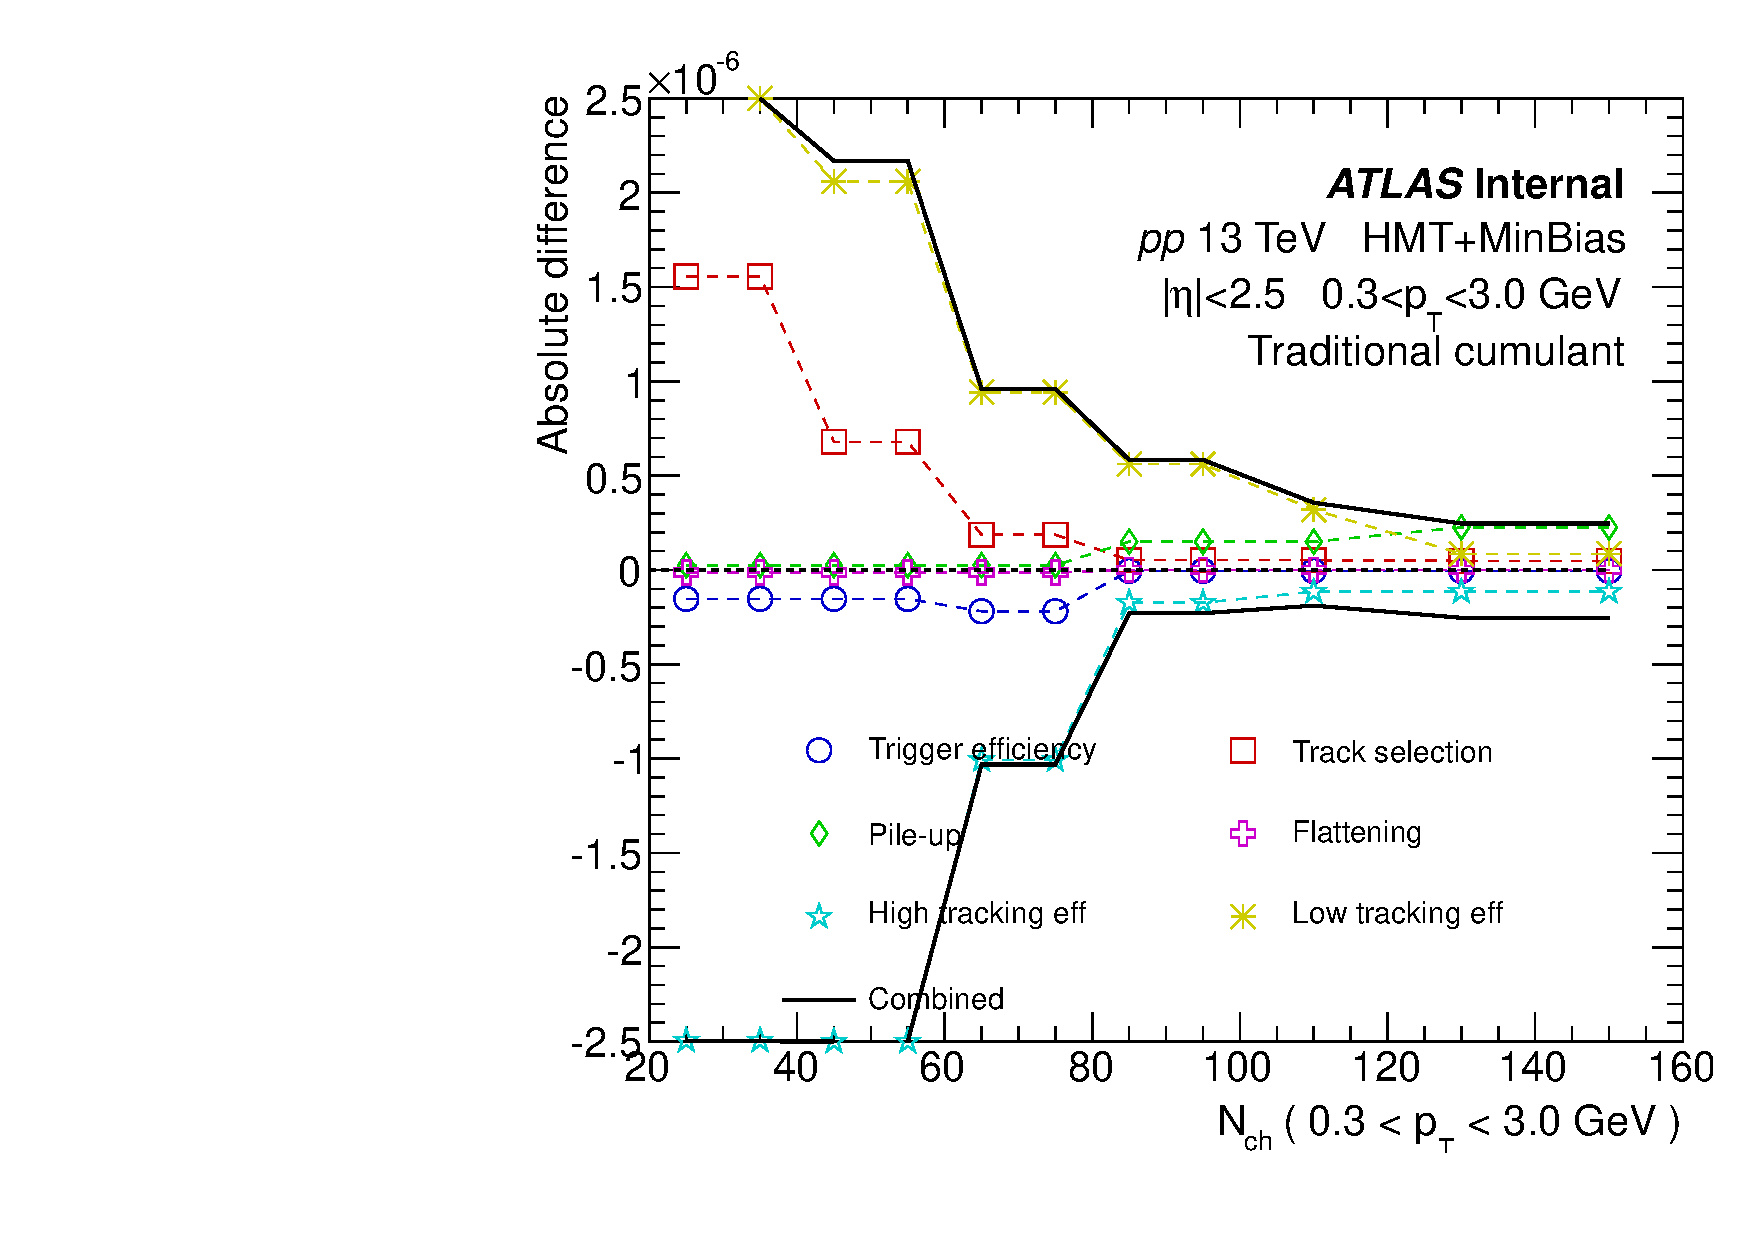
\includegraphics[width=0.3\linewidth]{figs/sec_sys/pp13/sys_pp13_NNNN_Har0_Pt0_Cls0.pdf}
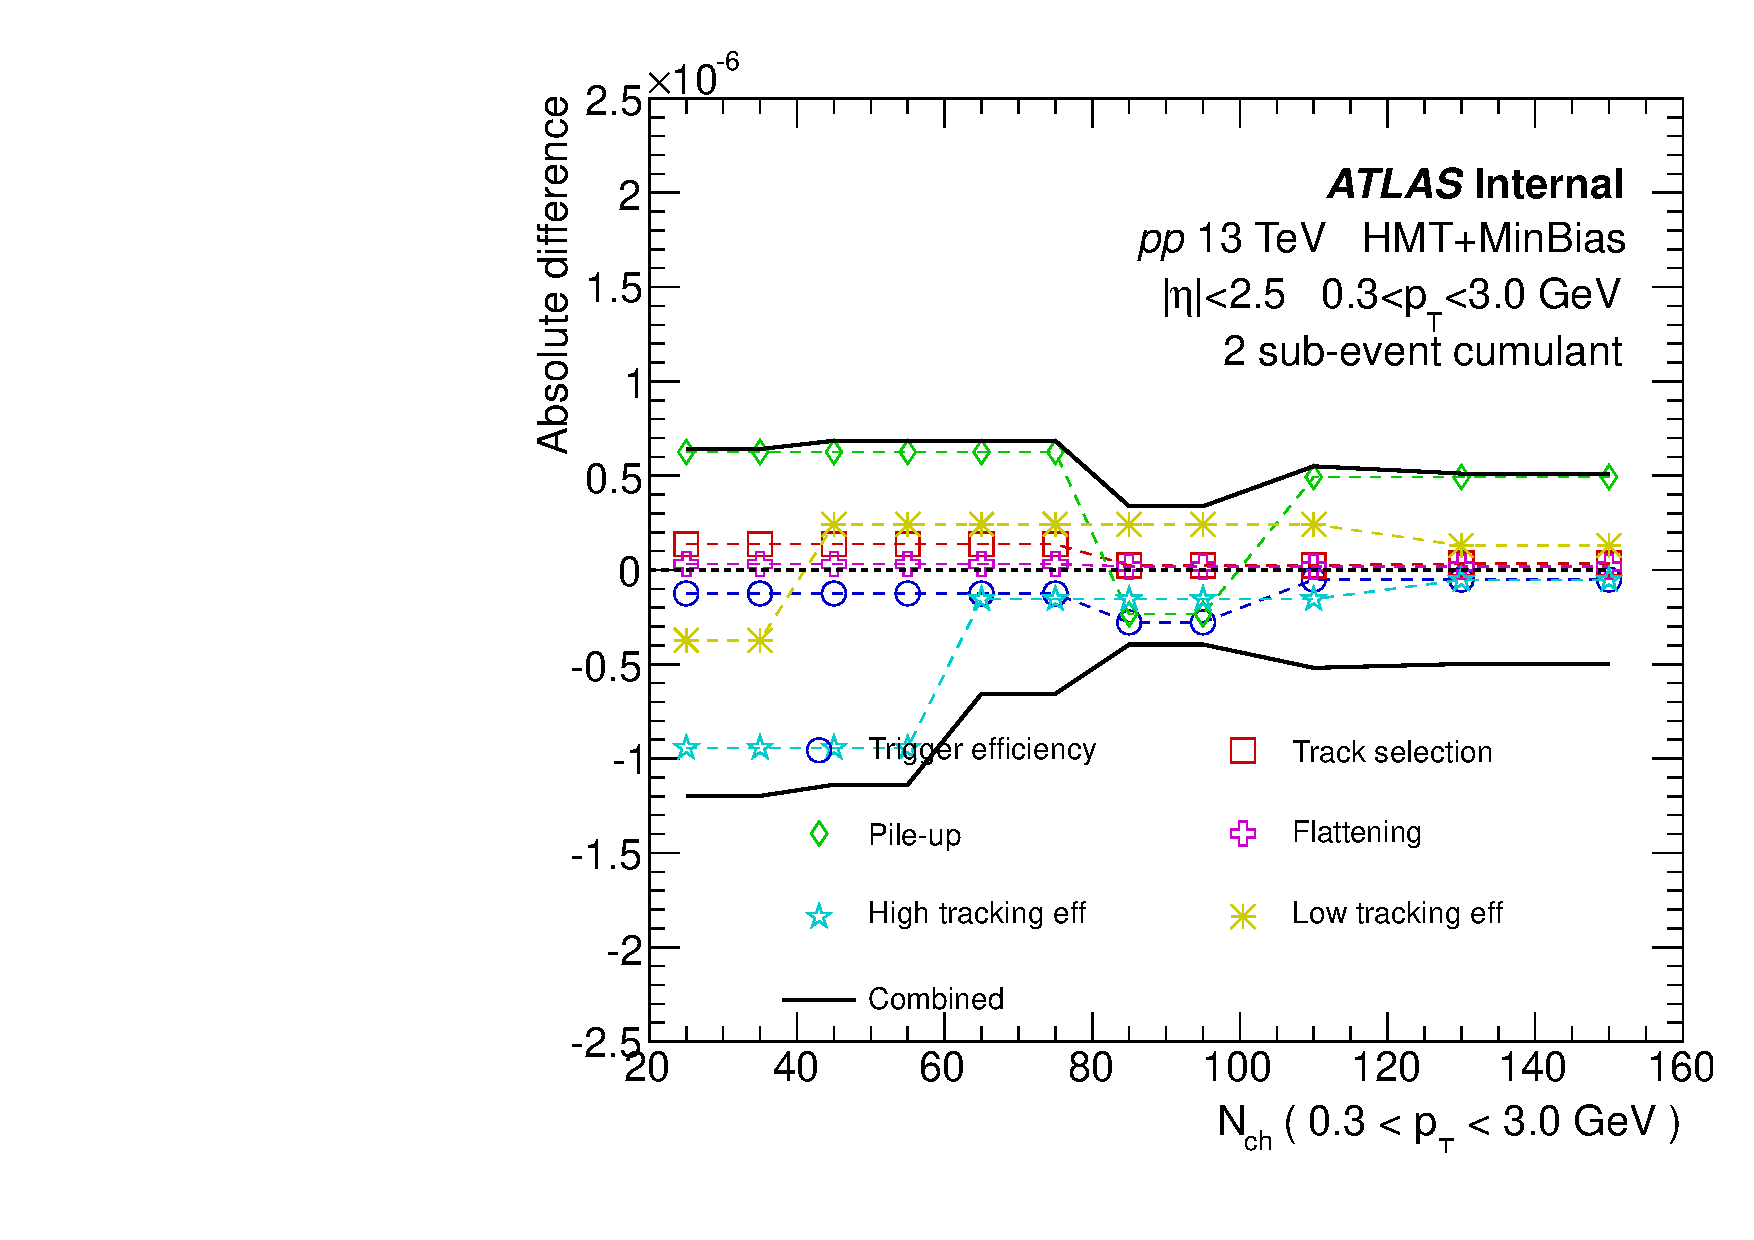
\includegraphics[width=0.3\linewidth]{figs/sec_sys/pp13/sys_pp13_ABAB_Har0_Pt0_Cls0.pdf}
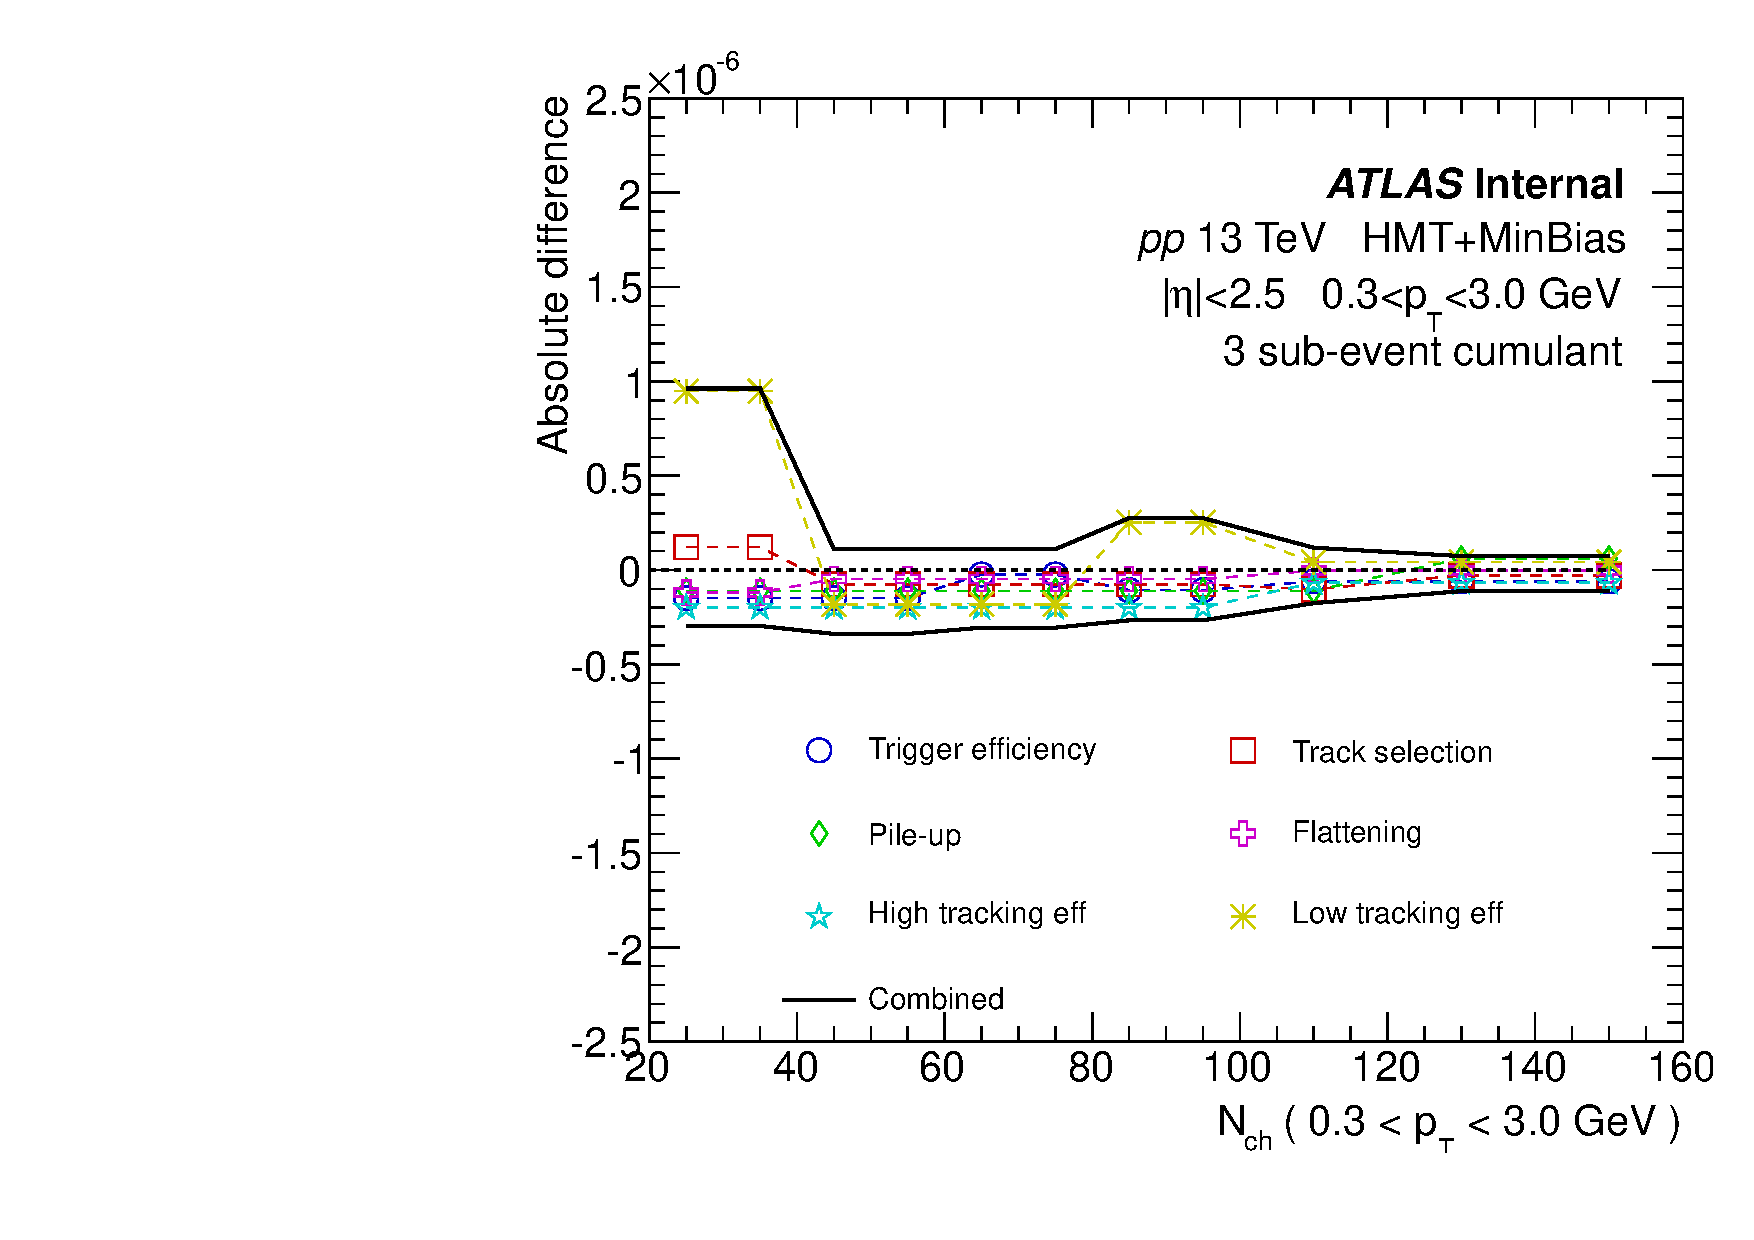
\includegraphics[width=0.3\linewidth]{figs/sec_sys/pp13/sys_pp13_ABAC_Har0_Pt0_Cls0.pdf}
\caption{Summary of systematics in 13 TeV $pp$, for three different methods, with $0.3<p_{T}<3.0$ GeV. The statistical errors are not shown for better readability. The total systematics combined systematics from trigger efficiency, track selection, pile-up effects, flattening procedure and tracking efficiency.}
\label{fig:sys_pp13_sum_pt0}
\end{figure}
Fig.~\ref{fig:sys_pp13_sum_pt0} summarizes five major systematic sources with the traditional cumulant method. The Y-axis shows the absolute difference for each check. The dominating uncertainty comes from when lowering the tracking efficiency by its uncertainty. Since the tracking efficiency adds different weights to particles with different $p_{T}$, and the non-flow sources usually contains high $p_{T}$ particles, lowering the tracking efficiency will equivalently adding more weights to the particles with higher $p_{T}$, causing a larger non-flow contribution. Since there is significant residue non-flow with the traditional method, this is the reason why varying tracking efficiency has the largest uncertainty. The next leading uncertainty comes from track selection, and it becomes larger towards the low multiplicity region, where the fraction of non-flow contribution is larger. For other sources, the absolute differences are relatively smaller: within $0.2\times 10^{-6}$.

As a comparison, fig.~\ref{fig:sys_pp13_sum_pt0} summarizes five major systematic sources with the 2 sub-event cumulant method. The Y-axis shows the absolute difference for each check. The uncertainty from lower tracking efficiency is much smaller than traditional cumulant method, since 2 sub-event method already largely suppressed the short-range non-flow sources. The uncertainty from the pile-up effects becomes larger and dominates the high multiplicity region, but that is partially due to a larger statistical errors (not shown in the plots for better readability) with the sub-event method. But in any case, the systematic from pile-up effects is still quoted even with large statistical errors. Overall, the combined systematics are within $0.5\times 10^{-6}$.

In the end, the summary of systematics from 3 sub-event method is shown in Fig.~\ref{fig:sys_pp13_sum_pt0}, which has the smallest systematic uncertainties among all 3 methods. The combined absolute difference is $0.3\times 10^{-6}$.

For completeness, the summary of systematics for 3 methods, but with higher $p_{T}$ region: $0.5<p_{T}<5.0$ GeV, are shown in Fig.~\ref{fig:sys_pp13_sum_pt1}. Compared with lower $p_{T}$ region, the uncertainties from all three methods grows larger. This is partially due to the fact that the statistical errors becomes larger thus the systematic fluctuation also becomes larger. But the main reason is that the fraction of non-flow contribution is larger when moving to the higher $p_{T}$ range. A comparison between systematics from three methods shows that 3 sub-event method still has the smallest uncertainty, consistent with the lower $p_{T}$ case.

\begin{figure}[H]
\centering
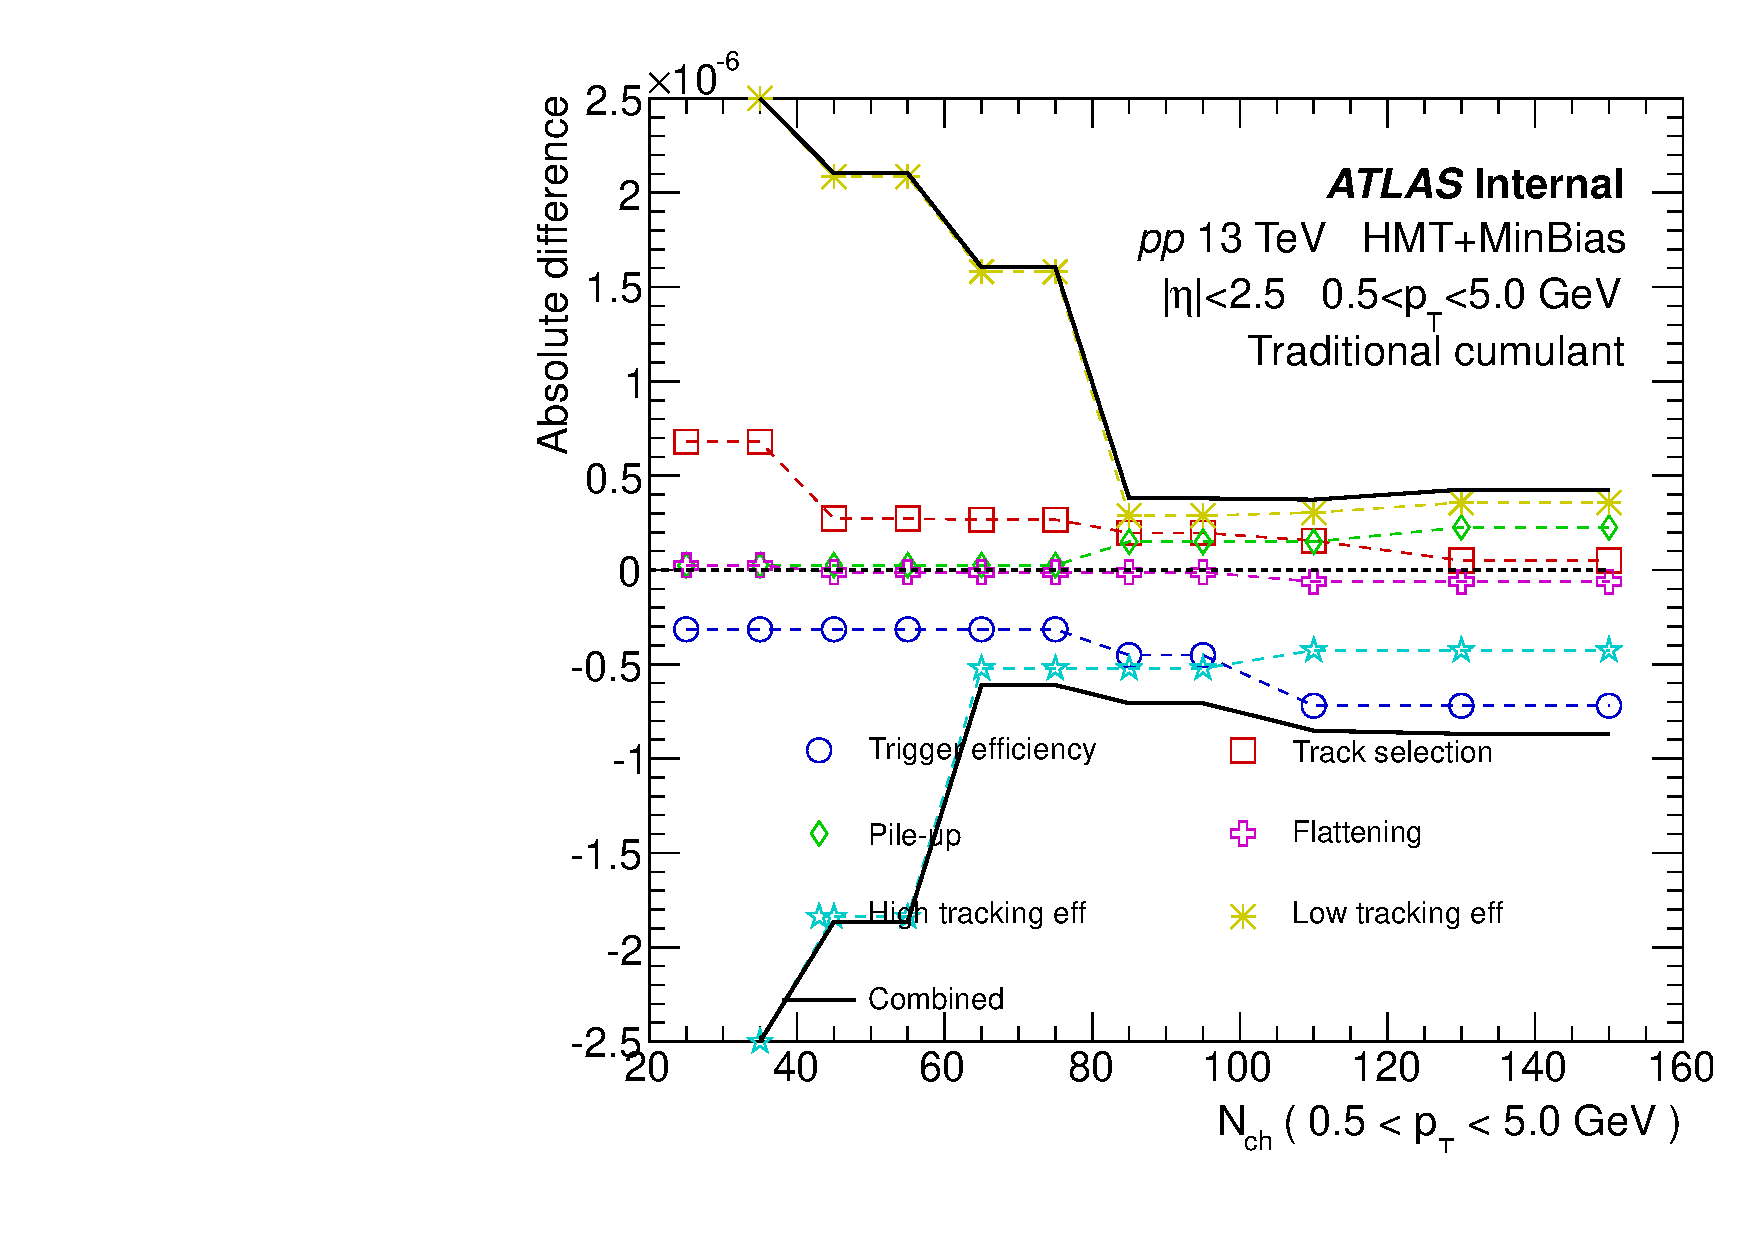
\includegraphics[width=0.3\linewidth]{figs/sec_sys/pp13/sys_pp13_NNNN_Har0_Pt1_Cls0.pdf}
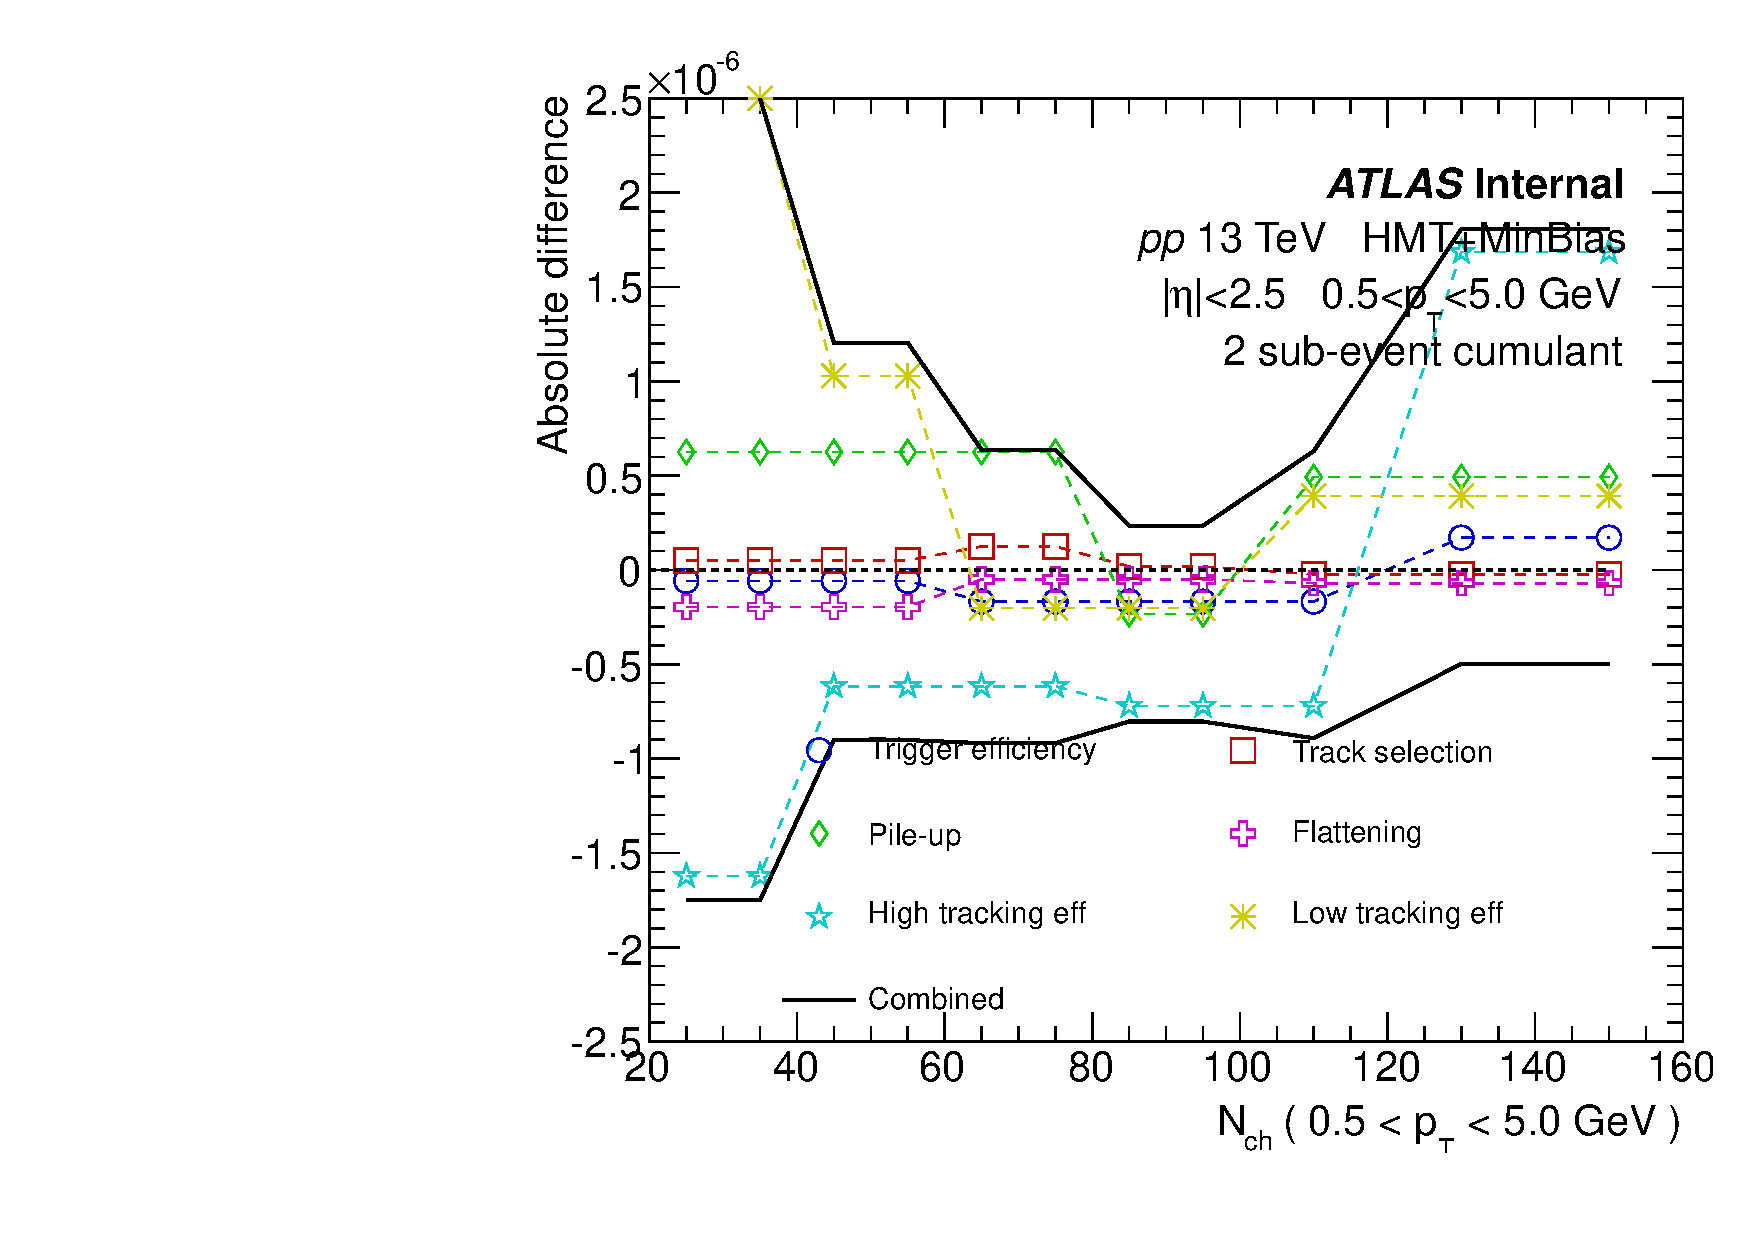
\includegraphics[width=0.3\linewidth]{figs/sec_sys/pp13/sys_pp13_ABAB_Har0_Pt1_Cls0.pdf}
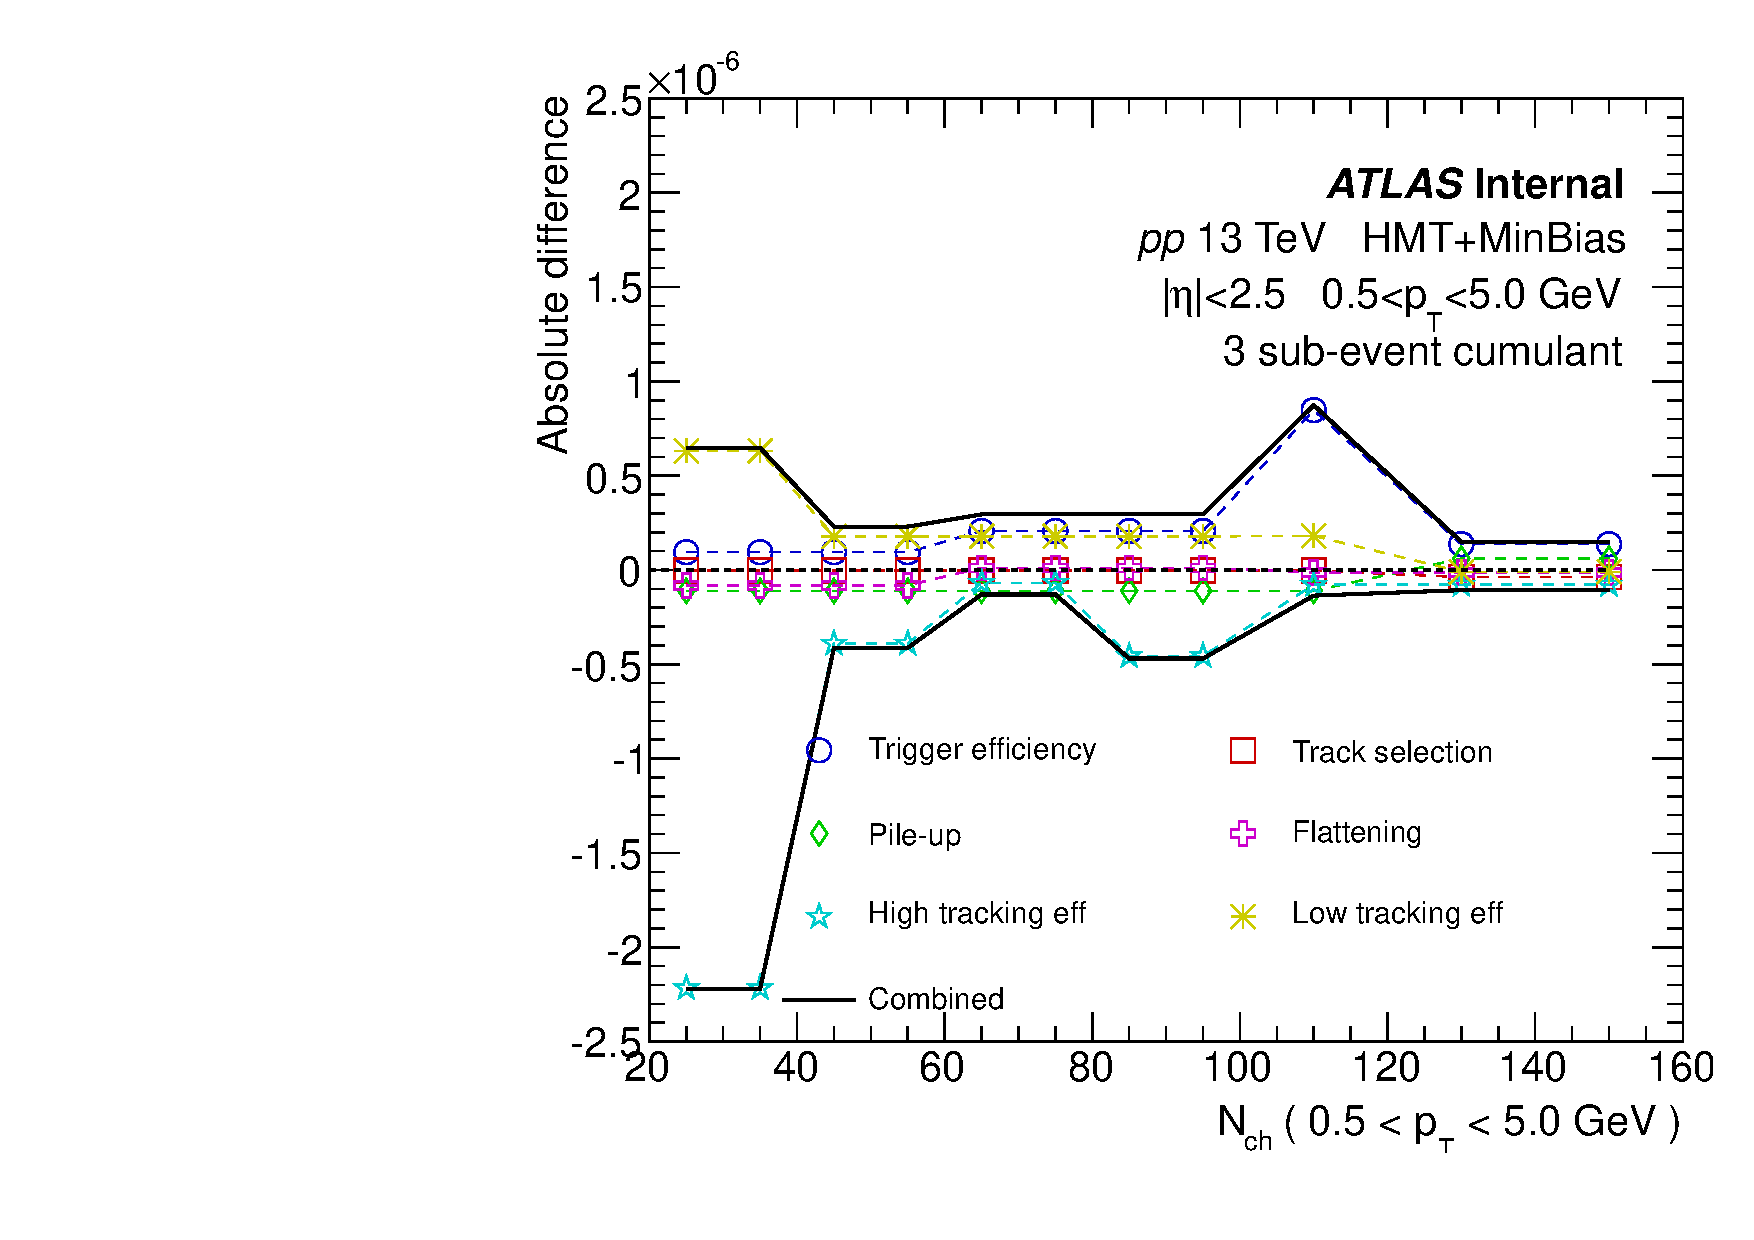
\includegraphics[width=0.3\linewidth]{figs/sec_sys/pp13/sys_pp13_ABAC_Har0_Pt1_Cls0.pdf}
\caption{Summary of systematics in 13 TeV $pp$, for 3 different cumulant methods, with $0.5<p_{T}<5.0$ GeV. The statistical errors are not shown for better readability.}
\label{fig:sys_pp13_sum_pt1}
\end{figure}



\subsection{$pp$ 5.02 TeV}
\subsubsection{Summary of systematics}
The systematic checks for 5.02 TeV $pp$ are identical to 13 TeV $pp$:
\begin{itemize}
\item Trigger efficiency: comparison between $50\%$ and $80\%$ HMT efficiency cut;
\item Track selection: tighten the $z_{0}$ and $d_{0}$ pointing cut to 1.0;
\item Pile-up effects: comparison between runs with $\mu<0.7$ and $\mu>1.5$;
\item Flattening procedure: comparison between with and without flattening in $\phi$;
\item High tracking efficiency: increasing tracking efficiency by its systematic uncertainty;
\item Low tracking efficiency: decreasing tracking efficiency by its systematic uncertainty;
\end{itemize}
For simplicity, we will not go through the systematics one by one, only the summary of systematics are shown in the following plots. The total statistics in 5 TeV $pp$ is much smaller than 13 TeV $pp$. Since the systematics will be larger due to larger statistical fluctuations. The results are re-binned to reduce the statistical fluctuation when necessary.

\begin{figure}[H]
\centering
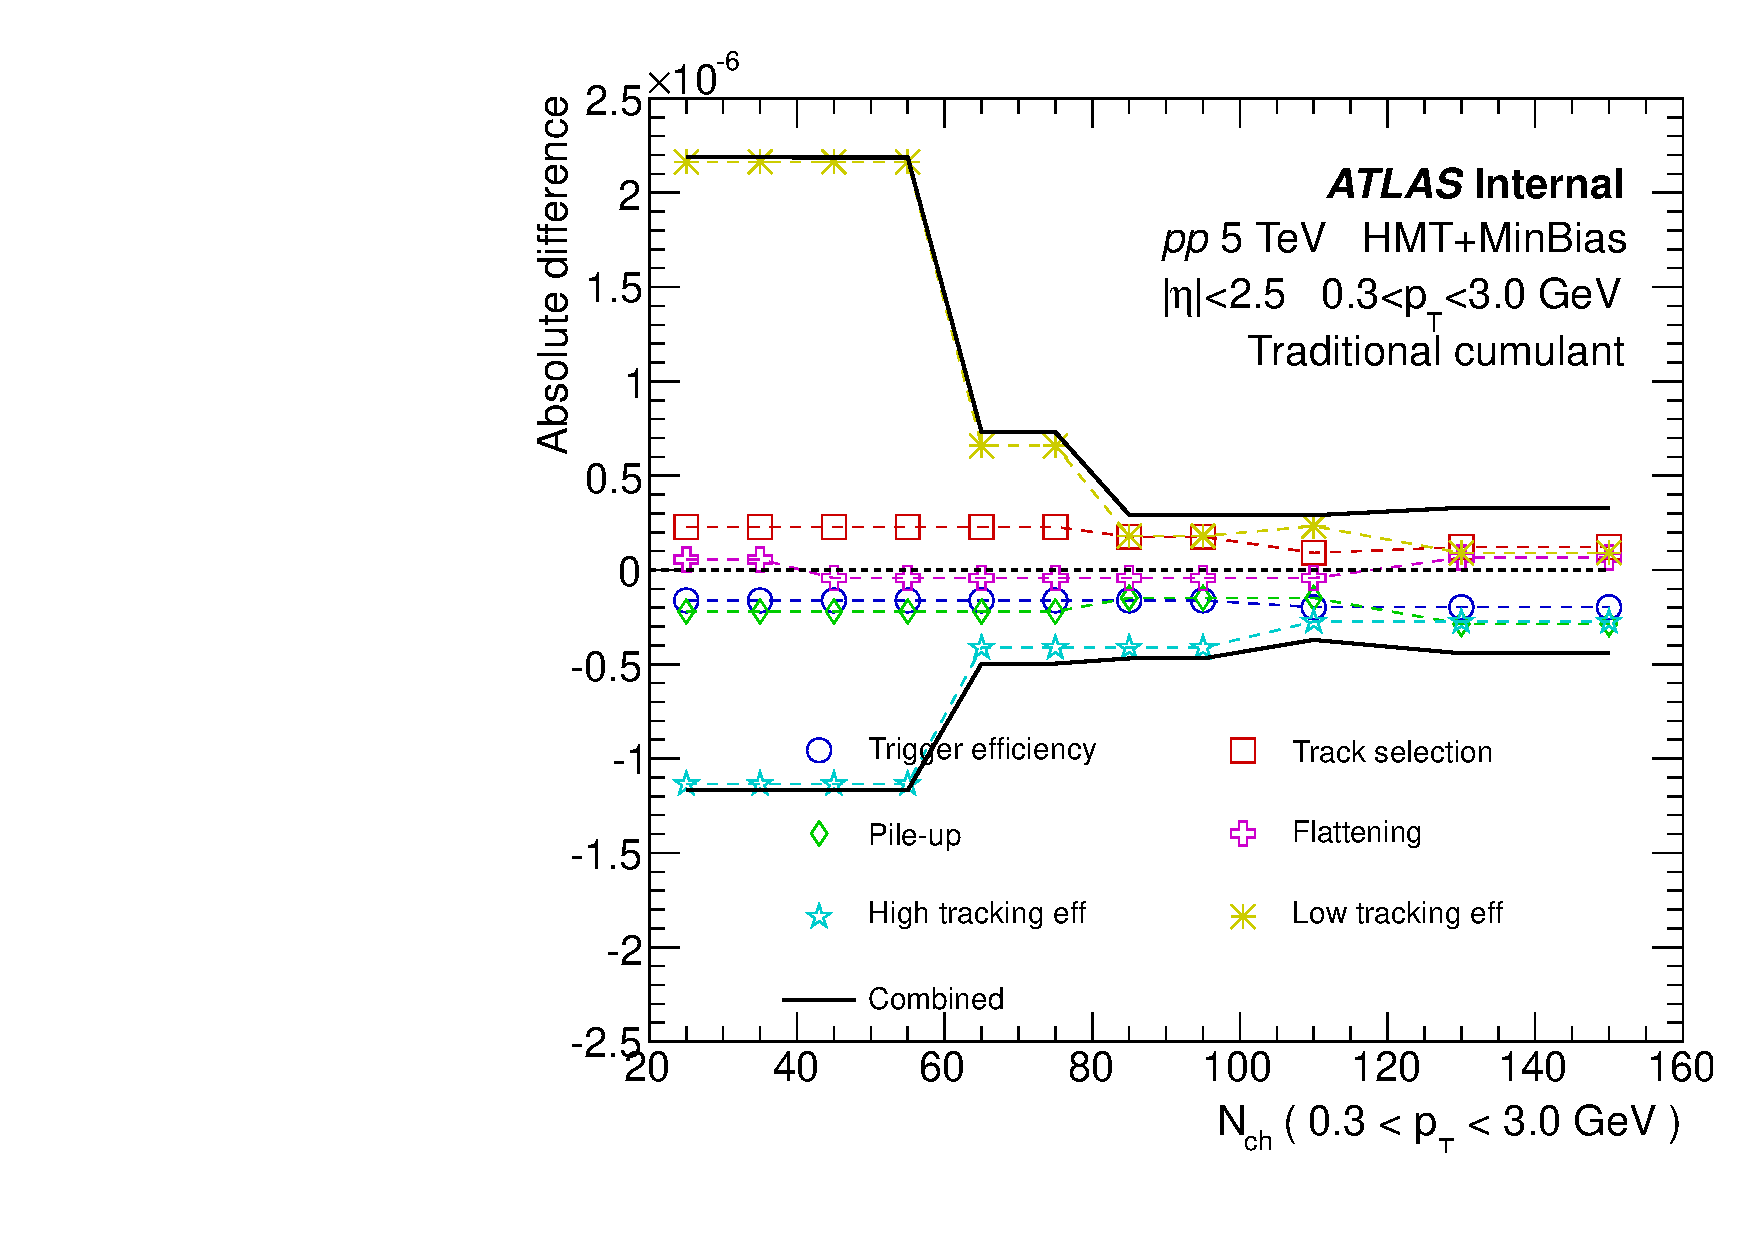
\includegraphics[width=0.3\linewidth]{figs/sec_sys/pp5/sys_pp5_NNNN_Har0_Pt0_Cls0.pdf}
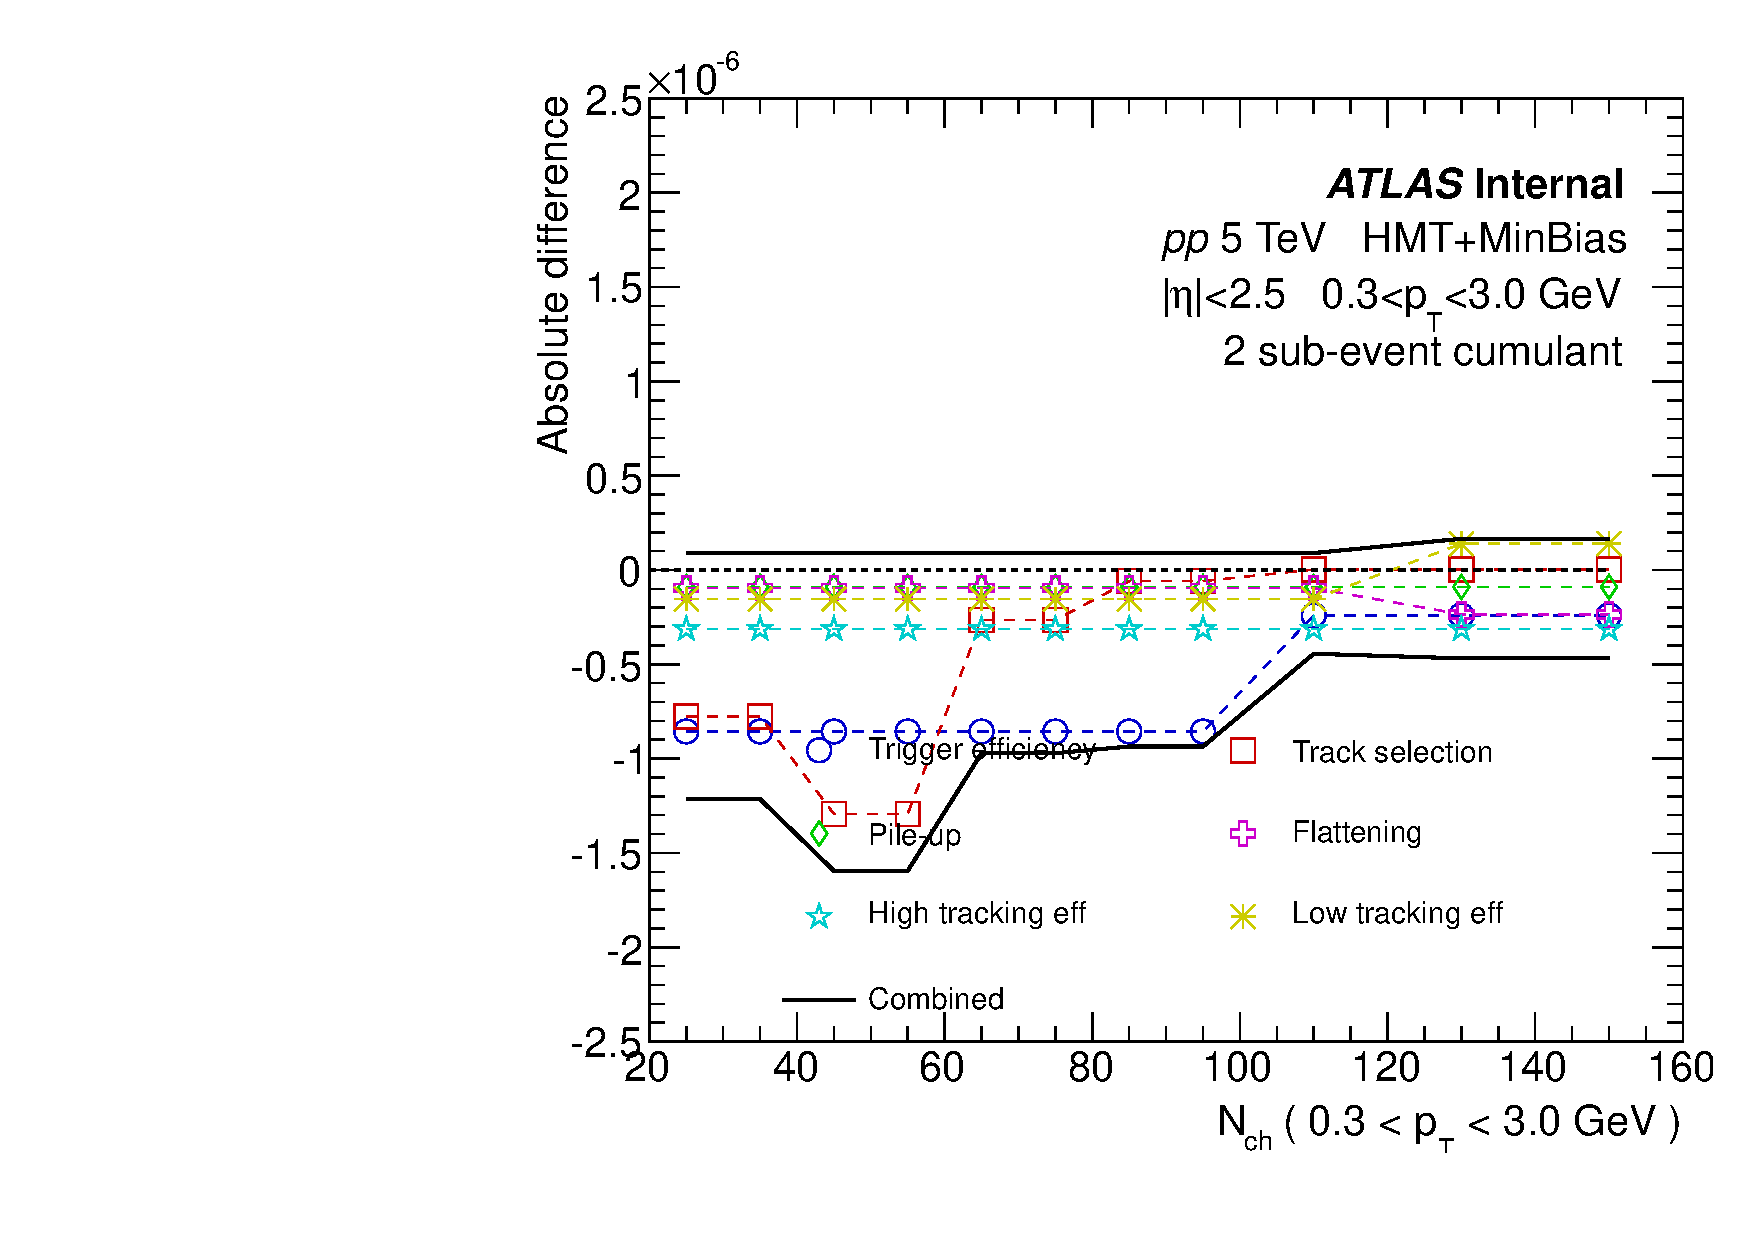
\includegraphics[width=0.3\linewidth]{figs/sec_sys/pp5/sys_pp5_ABAB_Har0_Pt0_Cls0.pdf}
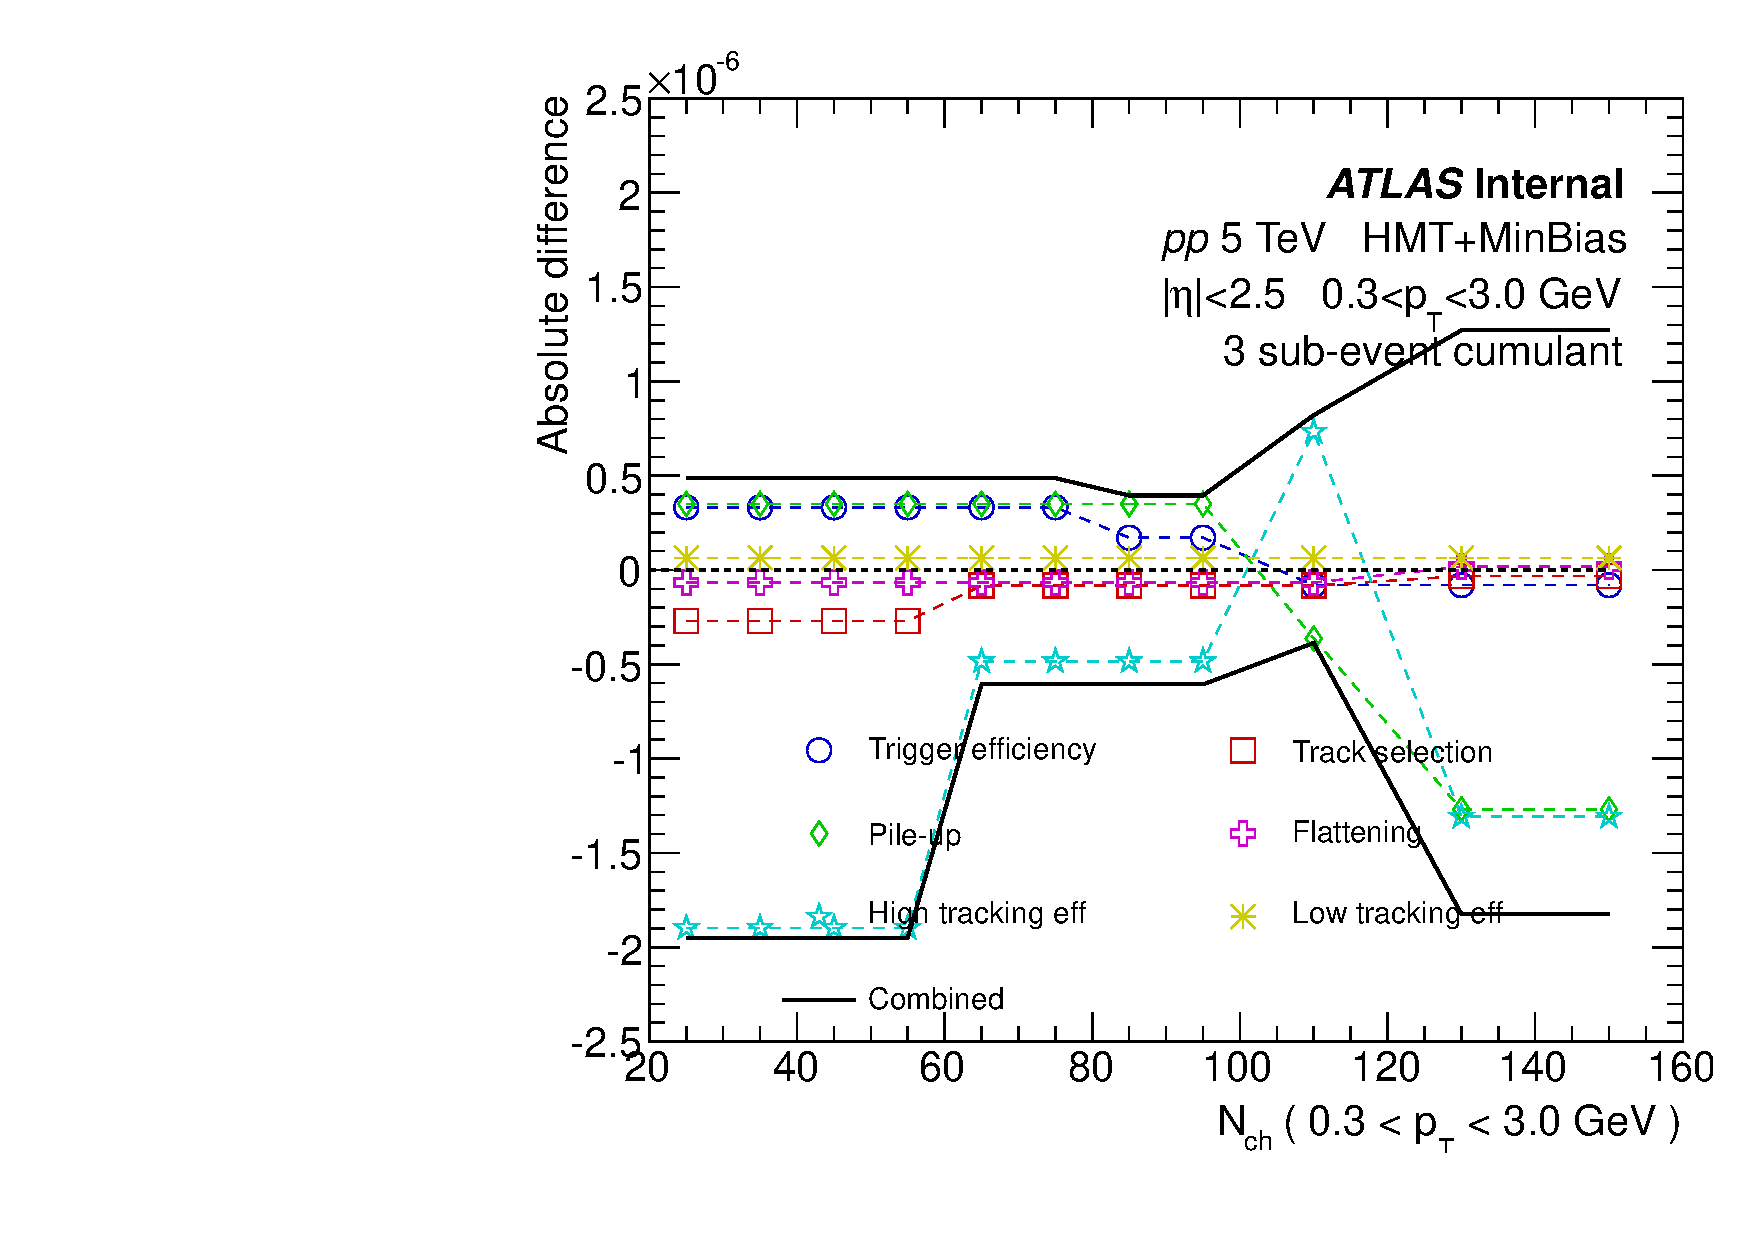
\includegraphics[width=0.3\linewidth]{figs/sec_sys/pp5/sys_pp5_ABAC_Har0_Pt0_Cls0.pdf}
\caption{Summary of systematics in 5.02 TeV $pp$, for three different cumulant methods, with $0.3<p_{T}<3.0$ GeV. The statistical errors are not shown for better readability.}
\label{fig:sys_pp5_sum_pt0}
\end{figure}

\begin{figure}[H]
\centering
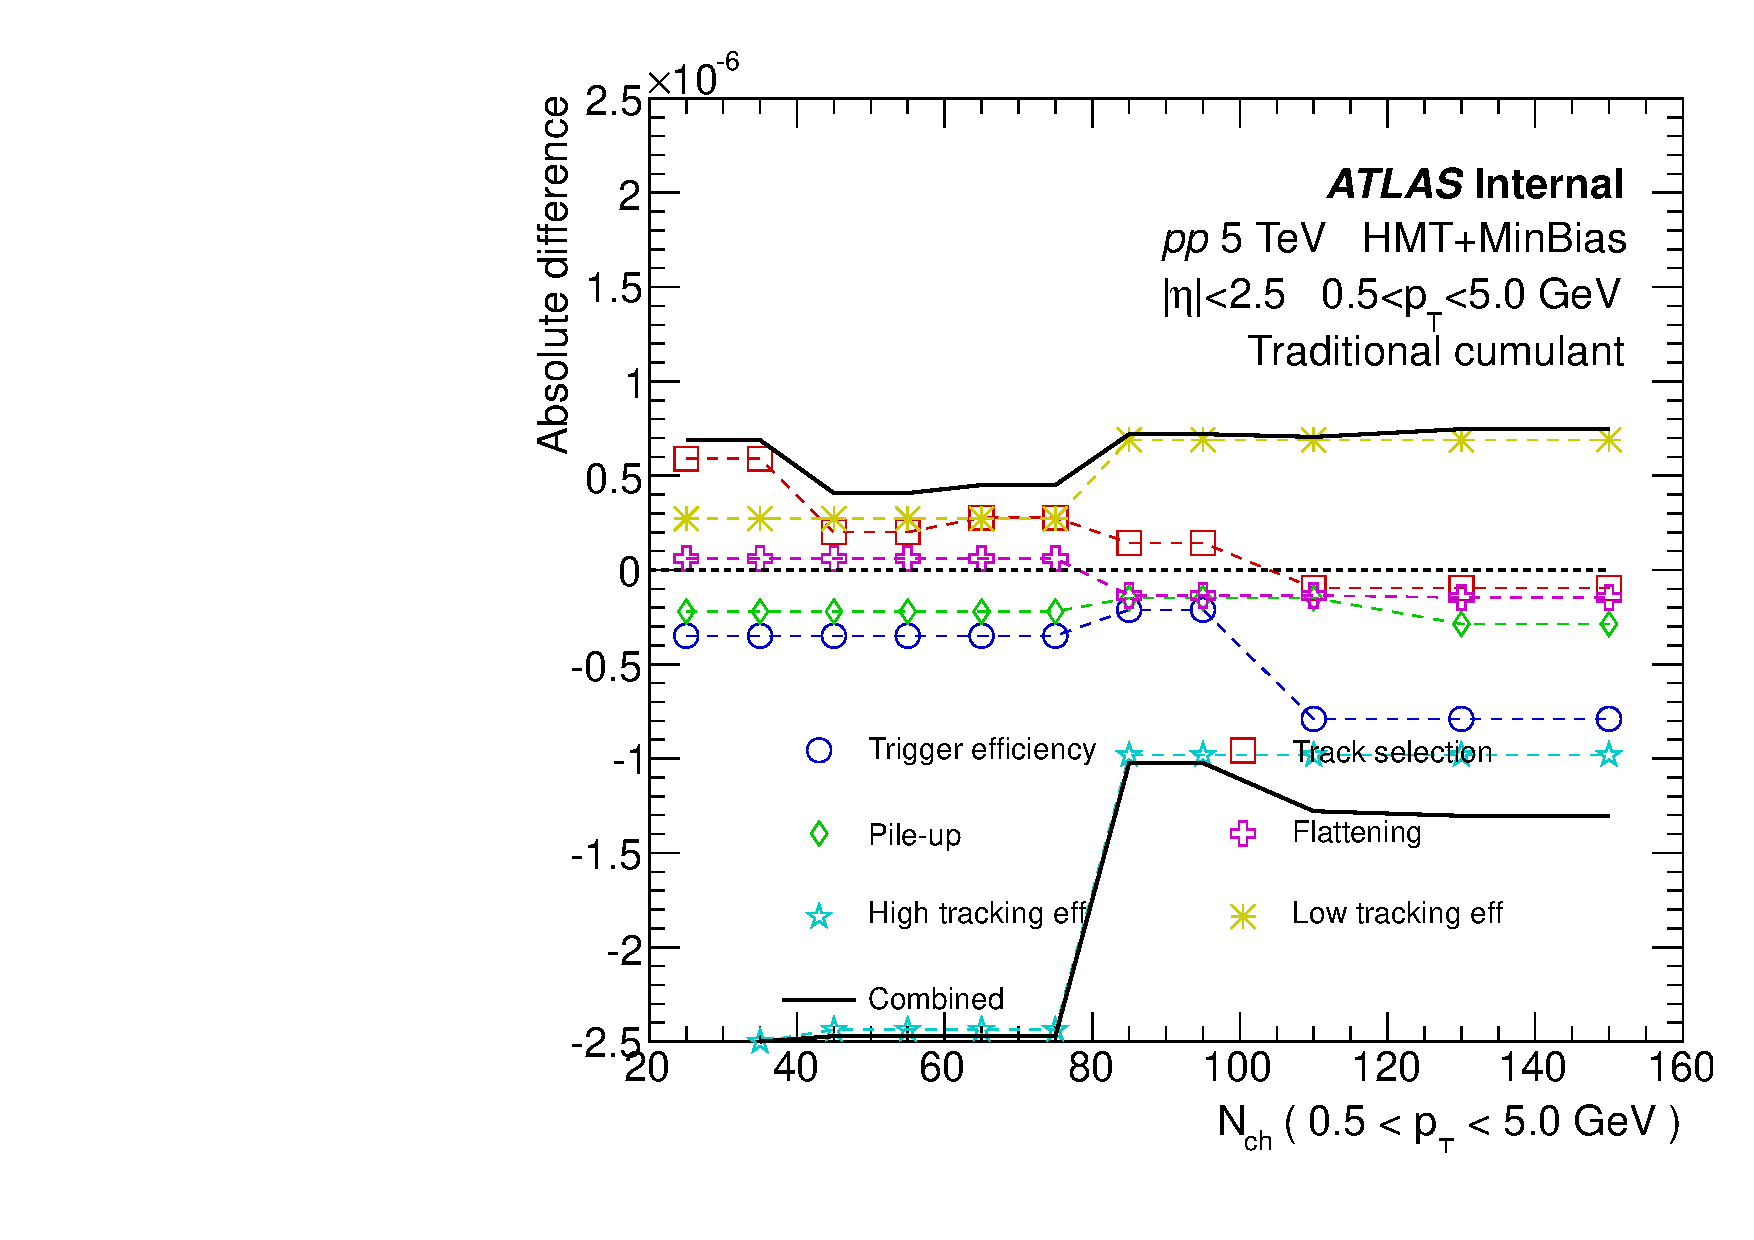
\includegraphics[width=0.3\linewidth]{figs/sec_sys/pp5/sys_pp5_NNNN_Har0_Pt1_Cls0.pdf}
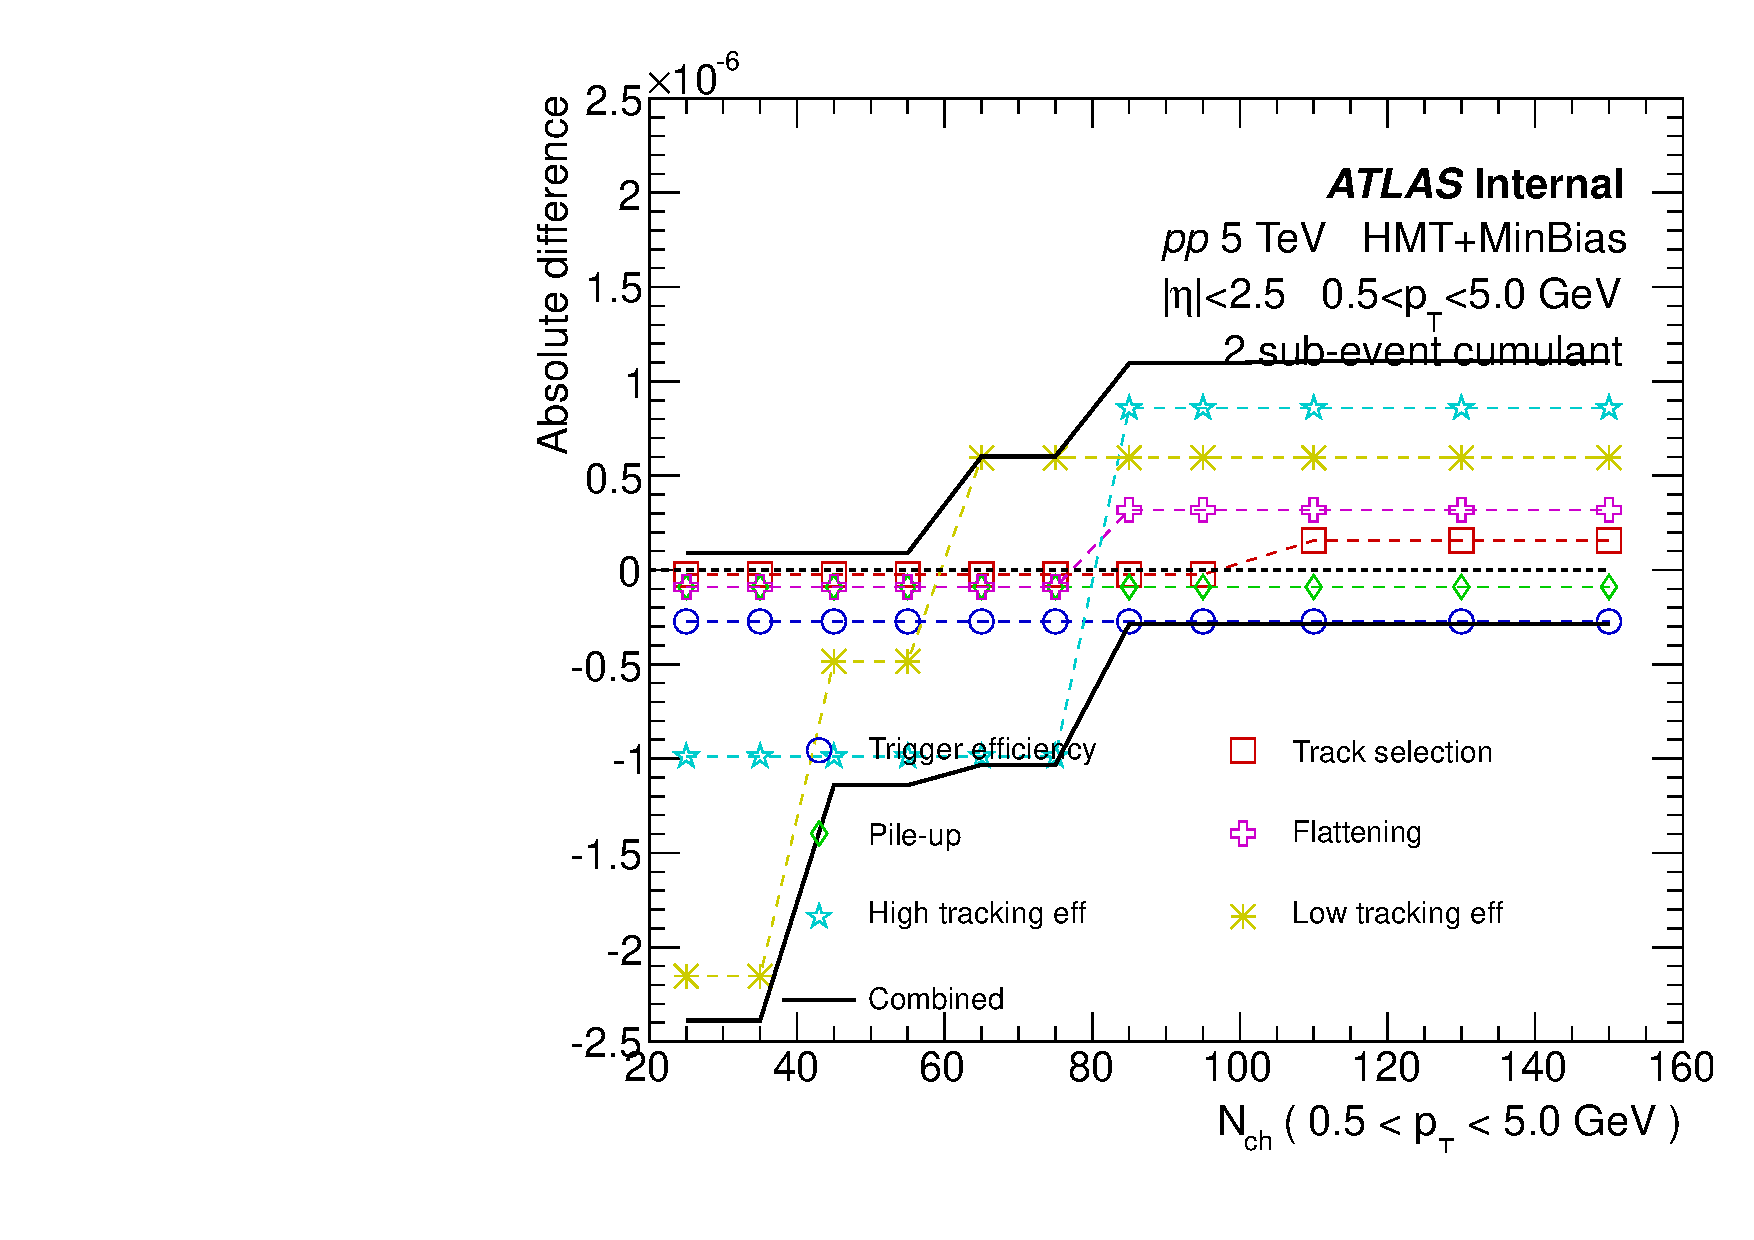
\includegraphics[width=0.3\linewidth]{figs/sec_sys/pp5/sys_pp5_ABAB_Har0_Pt1_Cls0.pdf}
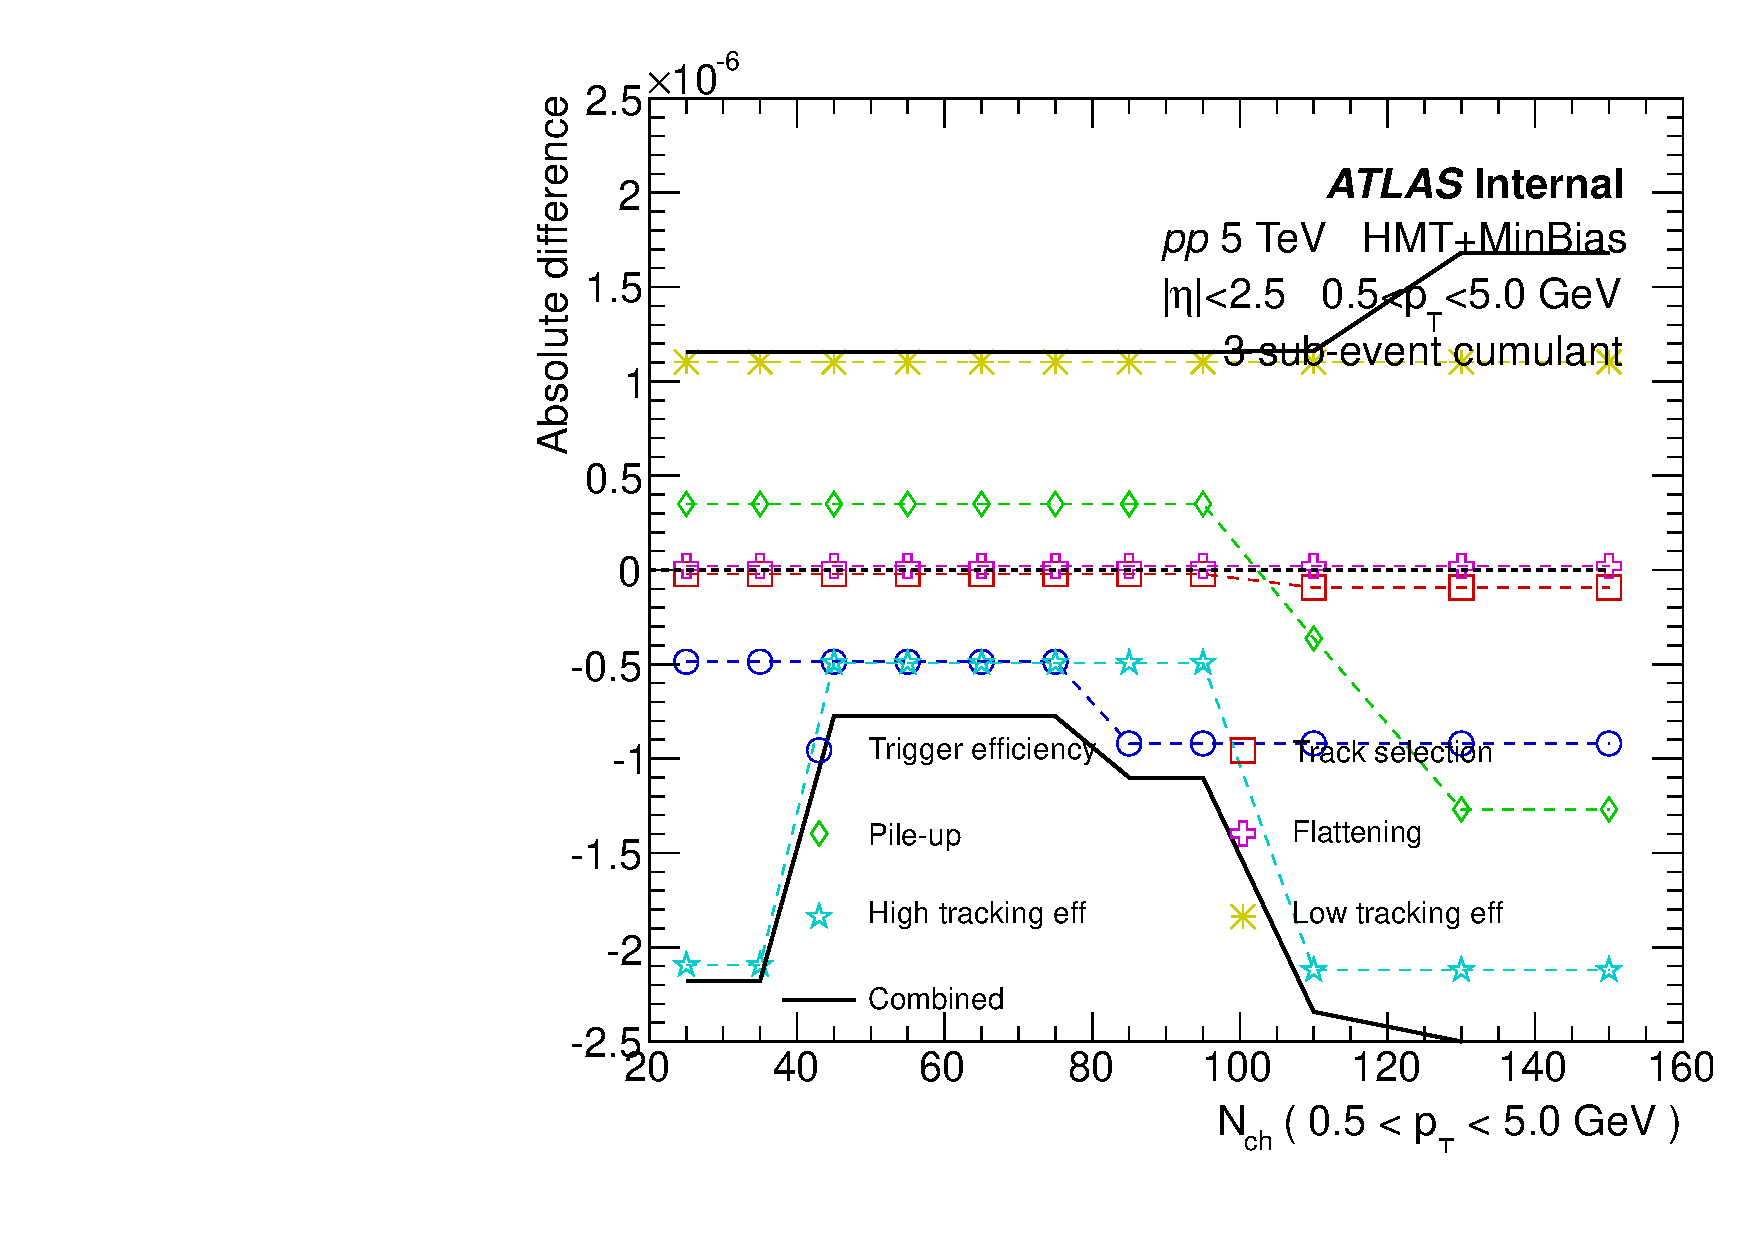
\includegraphics[width=0.3\linewidth]{figs/sec_sys/pp5/sys_pp5_ABAC_Har0_Pt1_Cls0.pdf}
\caption{Summary of systematics in 5.02 TeV $pp$, for three different cumulant methods, with $0.5<p_{T}<5.0$ GeV. The statistical errors are not shown for better readability.}
\label{fig:sys_pp5_sum_pt1}
\end{figure}




\subsection{$p$+Pb 5.02 TeV}
\subsubsection{Pileup rejection in run 1}
In the 2013 $p$+Pb run, the luminosity conditions provided by the LHC results in an average probability of $3\%$ that an event contains two or more $p$+Pb collisions (pileup). The pileup events are suppressed by the following two criteria:~\cite{atlas:9}
\begin{itemize}
\item Rejecting events containing more than one good reconstructed vertex (sum $p_{T} >$ 5 GeV);
\item A simple cut on the high tail end of the ZDC signal distribution;
\end{itemize}

\begin{figure}[H]
\centering
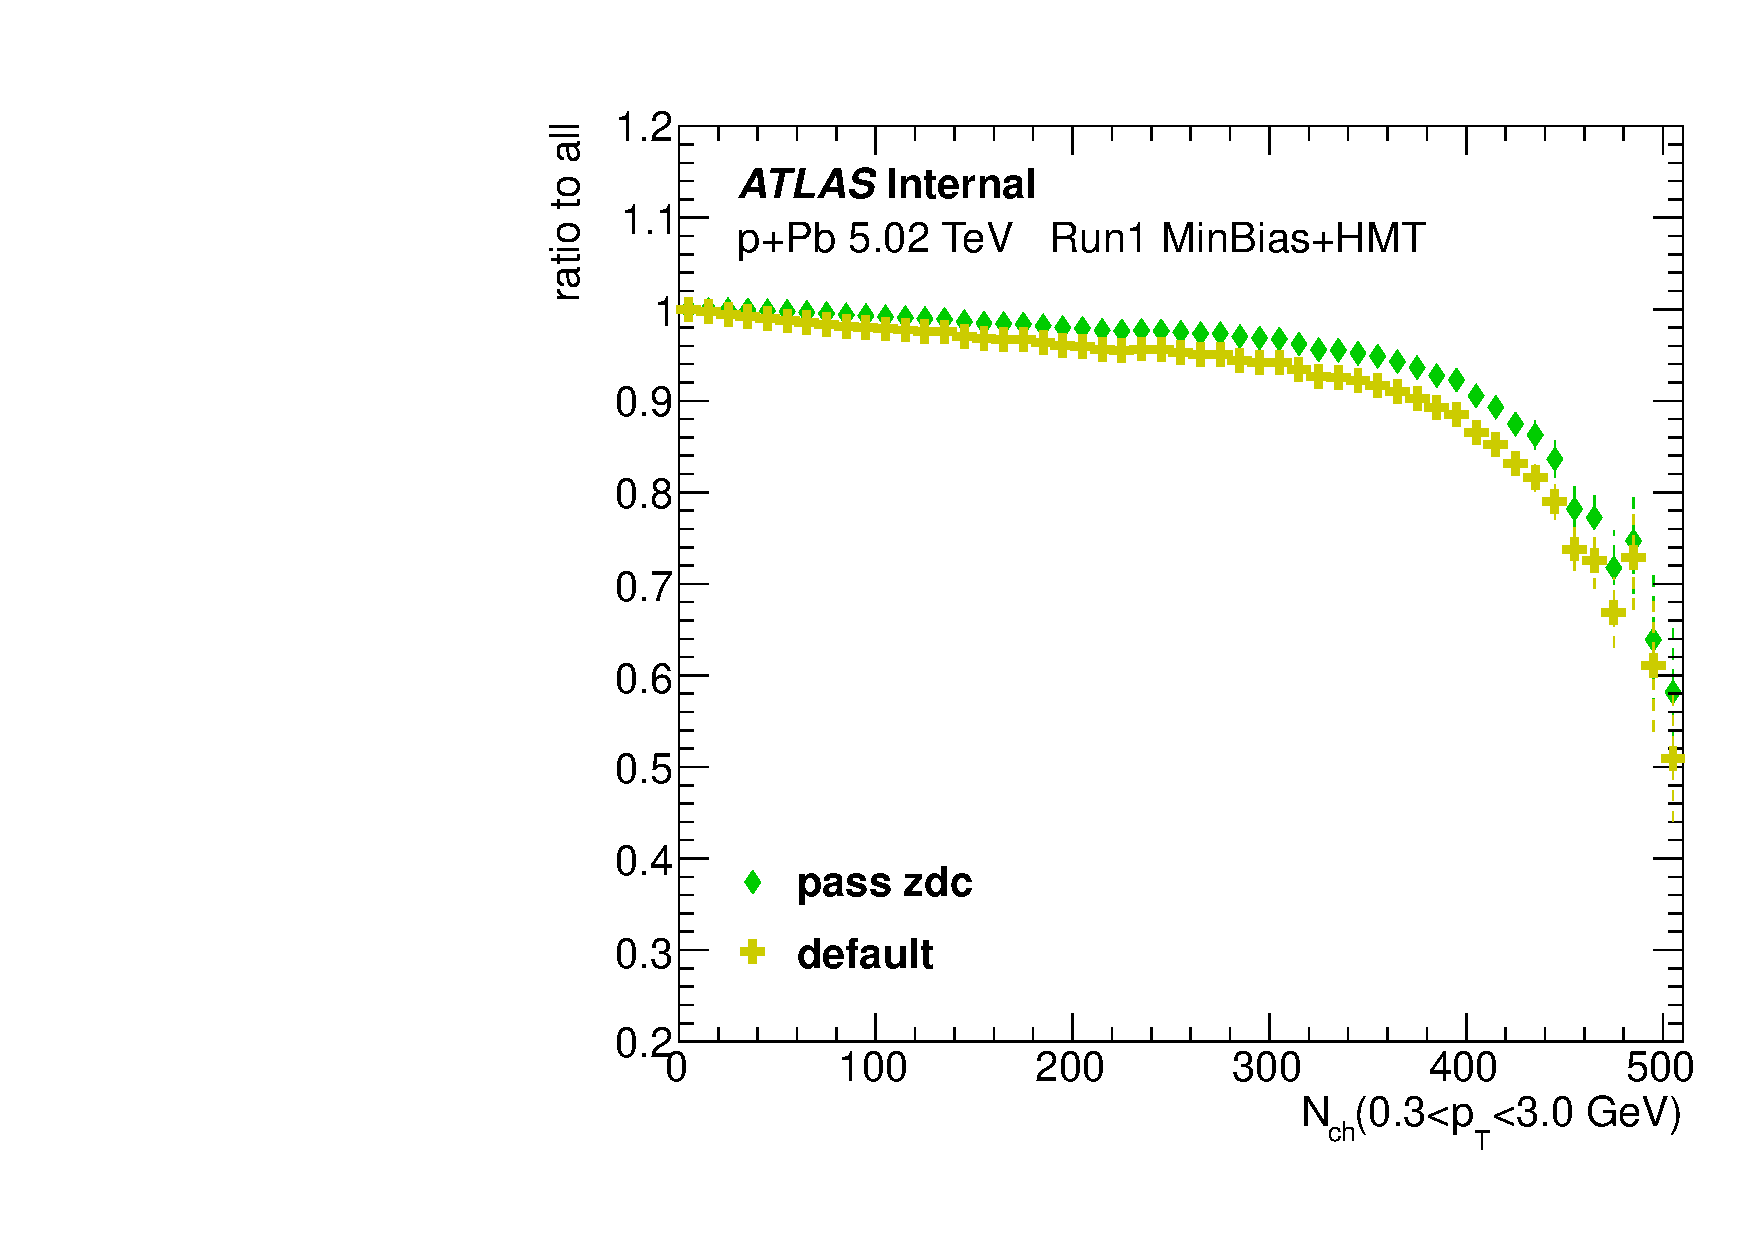
\includegraphics[width=0.45\linewidth]{figs/sec_sys/pPb5/PU_cnt_Pt0.pdf}
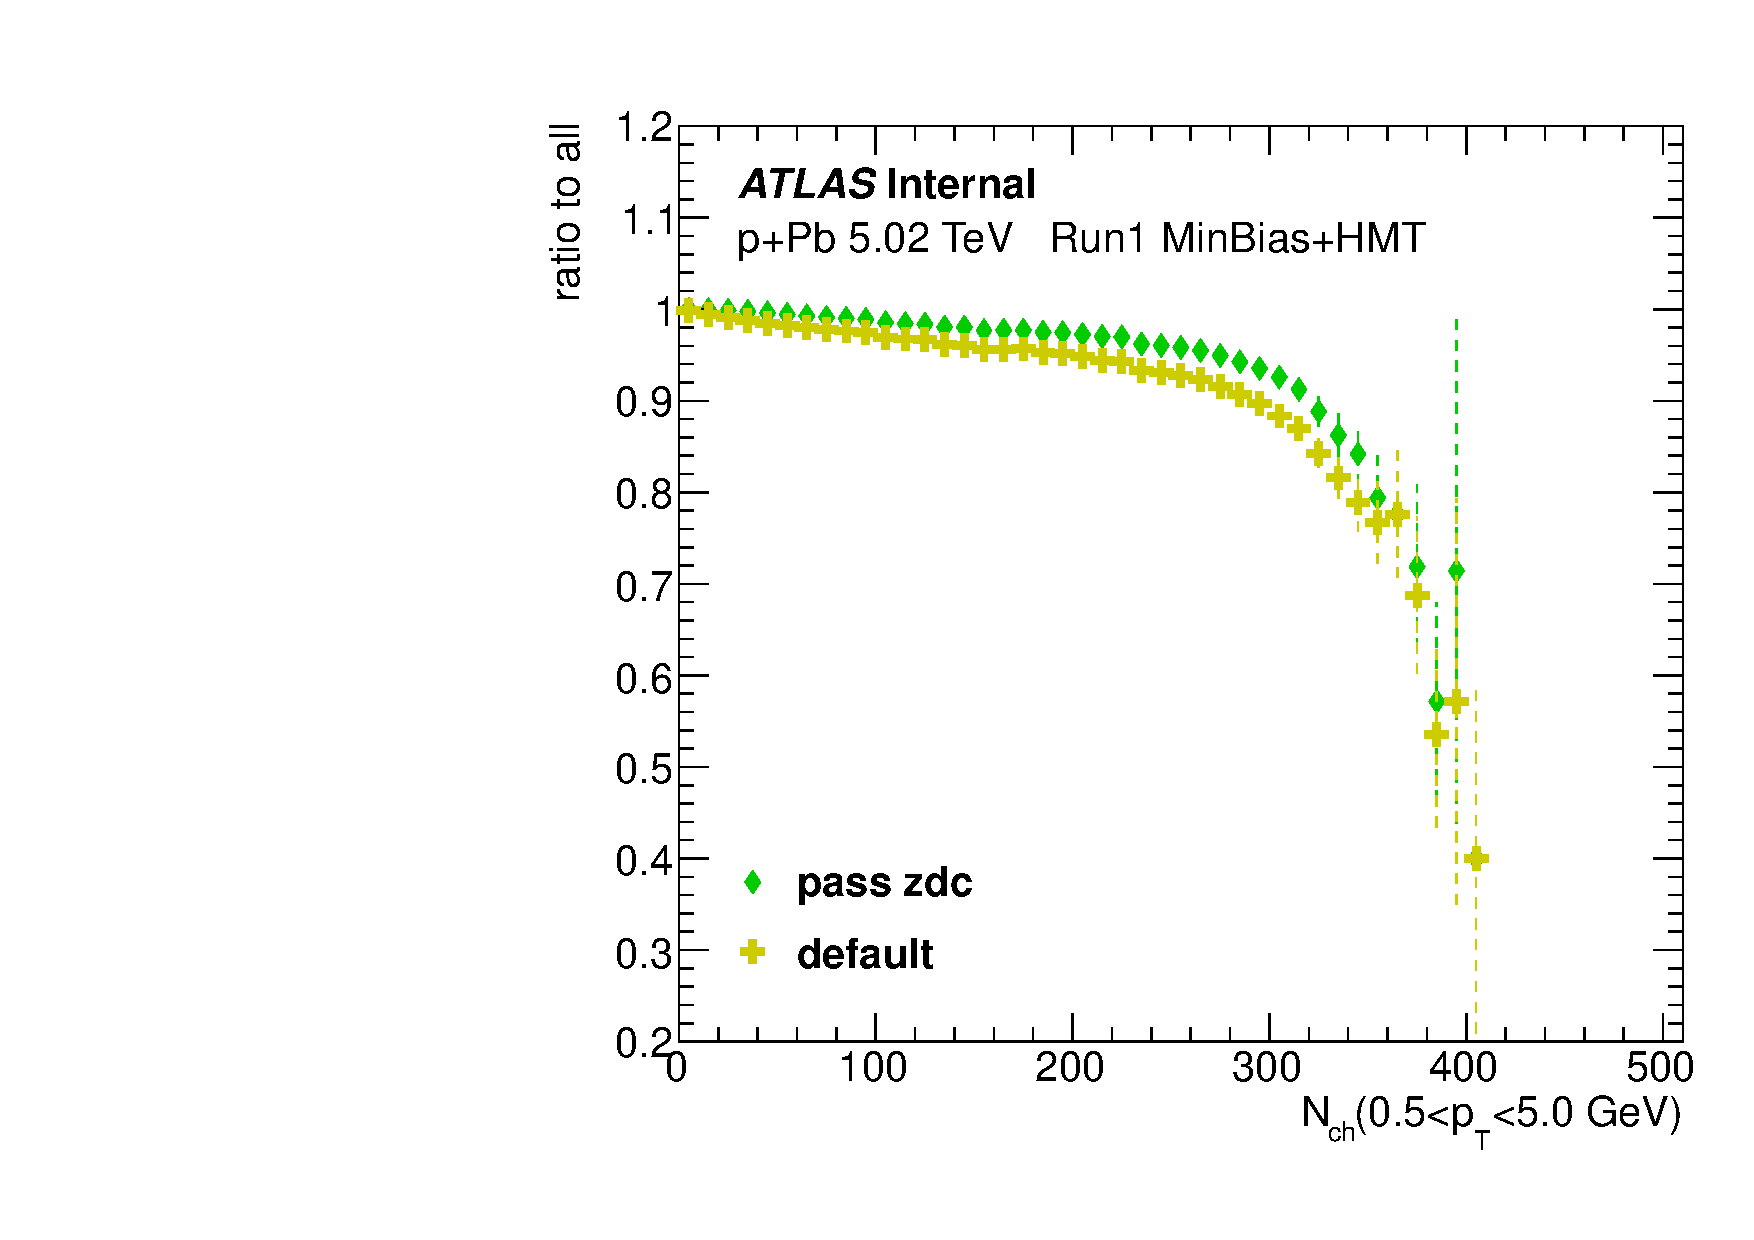
\includegraphics[width=0.45\linewidth]{figs/sec_sys/pPb5/PU_cnt_Pt1.pdf}
\caption{Fractions of remaining events after ZDC cut and additional vertex cut (default), in Run 1 5.02 TeV $p$+Pb, for two $p_{T}$ ranges: $0.3<p_{T}<3.0$ GeV (left) and $0.5<p_{T}<5.0$ GeV (right).}
\label{fig:chk_PU_cnt}
\end{figure}
Fig.~\ref{fig:chk_PU_cnt} shows the fractions of remaining events after ZDC cut and additional vertex cut (default), for two $p_{T}$ ranges. In this analysis, the default procedure is with both vertex and ZDC cut. As expected, the fraction of pileup events increase as $N_{ch}$ increases, reaches $~50\%$ in the highest $N_{ch}$ region. Compared with ZDC cut, additional vertex cut can further reject pileup events.

\begin{figure}[H]
\centering
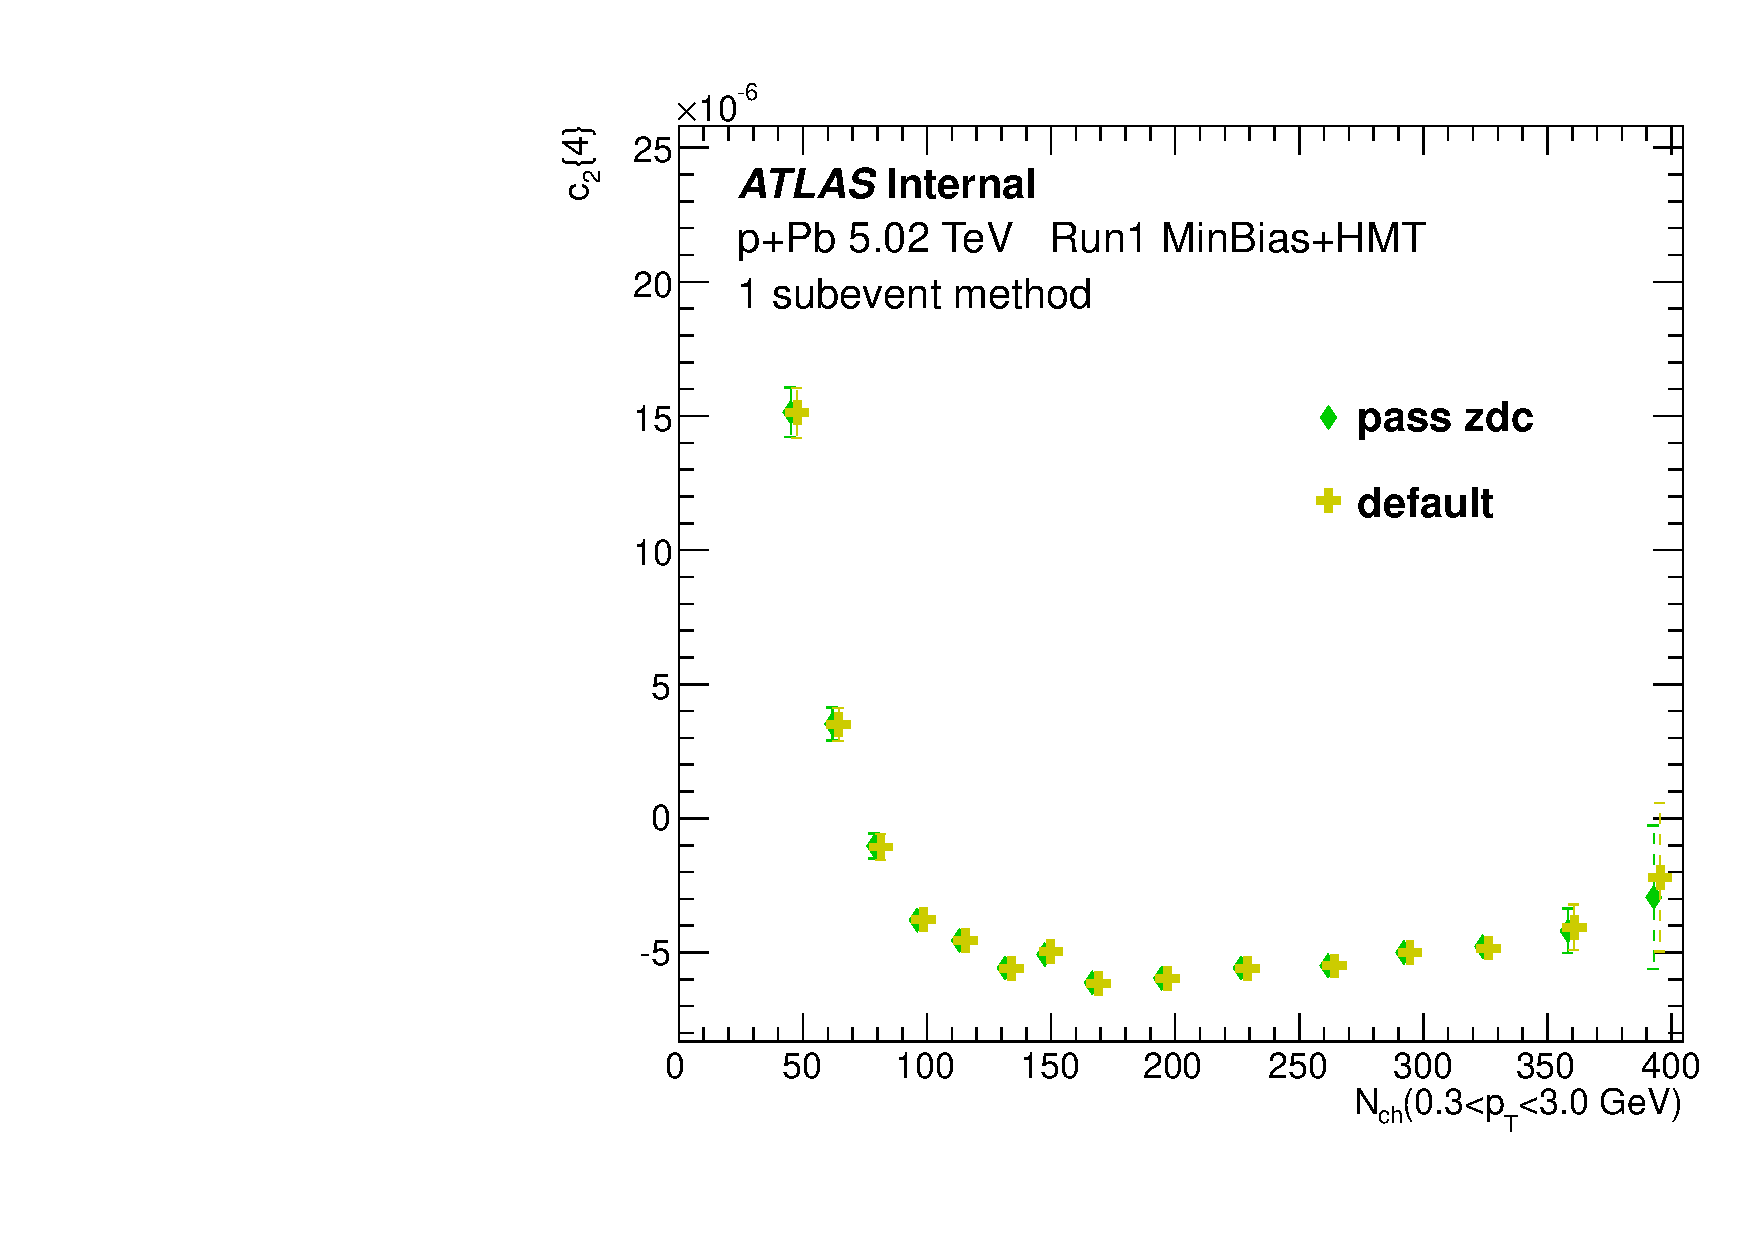
\includegraphics[width=0.45\linewidth]{figs/sec_sys/pPb5/PU_c4_1sub_Pt0.pdf}
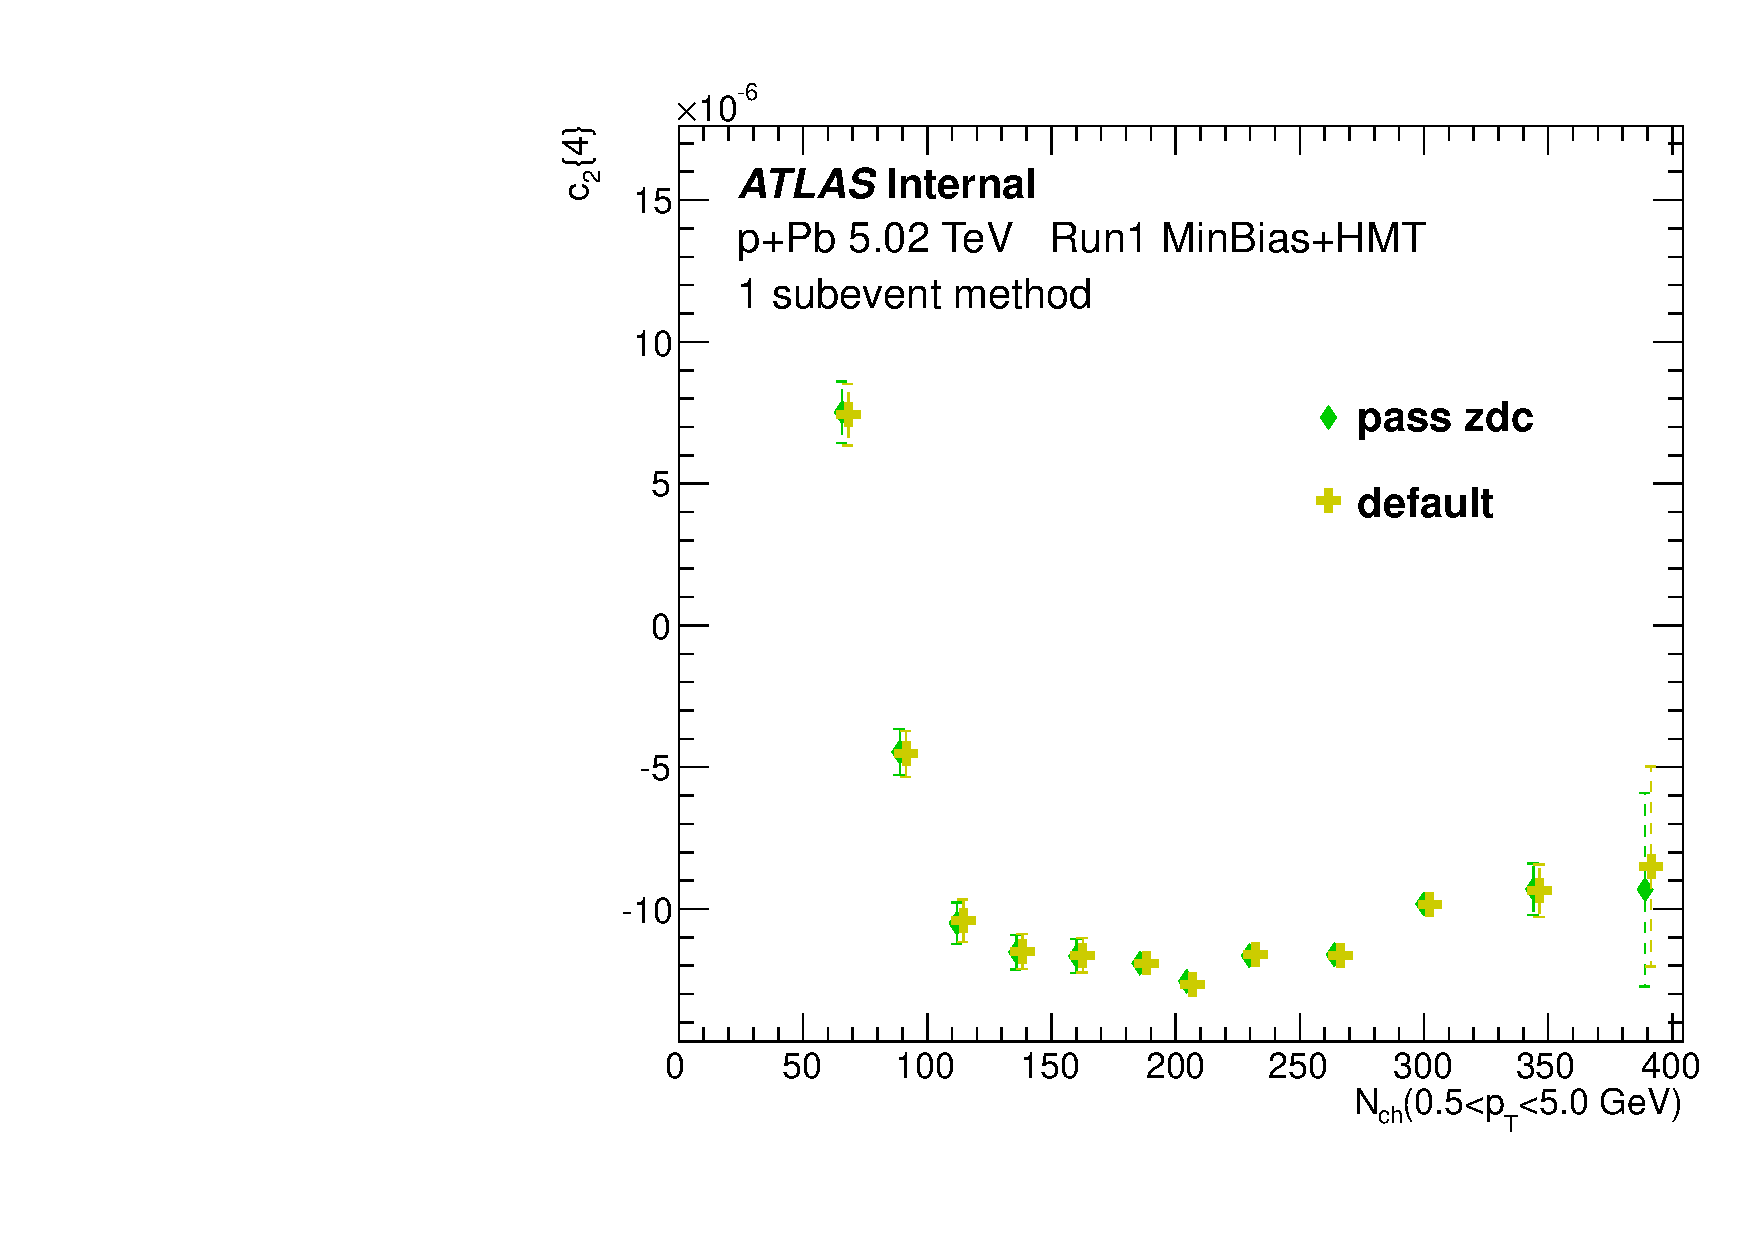
\includegraphics[width=0.45\linewidth]{figs/sec_sys/pPb5/PU_c4_1sub_Pt1.pdf}
\caption{Comparisons of $c_{2}\{4\}$ calculated in events with different pileup rejections, after ZDC cut and additional vertex cut (default), with standard cumulant method, in Run 1 5.02 TeV $p$+Pb, for two $p_{T}$ ranges: $0.3<p_{T}<3.0$ GeV (left) and $0.5<p_{T}<5.0$ GeV (right). The $x$ axis are shifted on purpose for better comparison.}
\label{fig:chk_PU_c24}
\end{figure}
To gain an idea how pileup rejection could affect the final results, Fig.~\ref{fig:chk_PU_c24} shows the comparisons of $c_{2}\{4\}$ calculated in events with different pileup rejections: after ZDC cut and additional vertex cut (default), with standard cumulant method. The results are very consistent between two cuts: even though additional vertex cut further cleans up pileup events, the results are already very stable even with the residual pileup events. The 2 and 3 subevent methods give similar behaviors but with larger errors.



\subsubsection{Summary of systematics}
The systematic checks for 5.02 TeV $p$+Pb are similar to $pp$, pile-up effects are replaced with run period dependence:
\begin{itemize}
\item Trigger efficiency: comparison between $50\%$ and $80\%$ HMT efficiency cut;
\item Track selection: tighten the $z_{0}$ and $d_{0}$ pointing cut;
\item Run period: comparison results before and after beam reversal;
\item Flattening procedure: comparison between with and without flattening in $\phi$;
\item High tracking efficiency: increasing tracking efficiency by its systematic uncertainty;
\item Low tracking efficiency: decreasing tracking efficiency by its systematic uncertainty;
\end{itemize}
For simplicity, we will not go through the systematics one by one, only the summary of systematics are shown in the following plots. 

\begin{figure}[H]
\centering
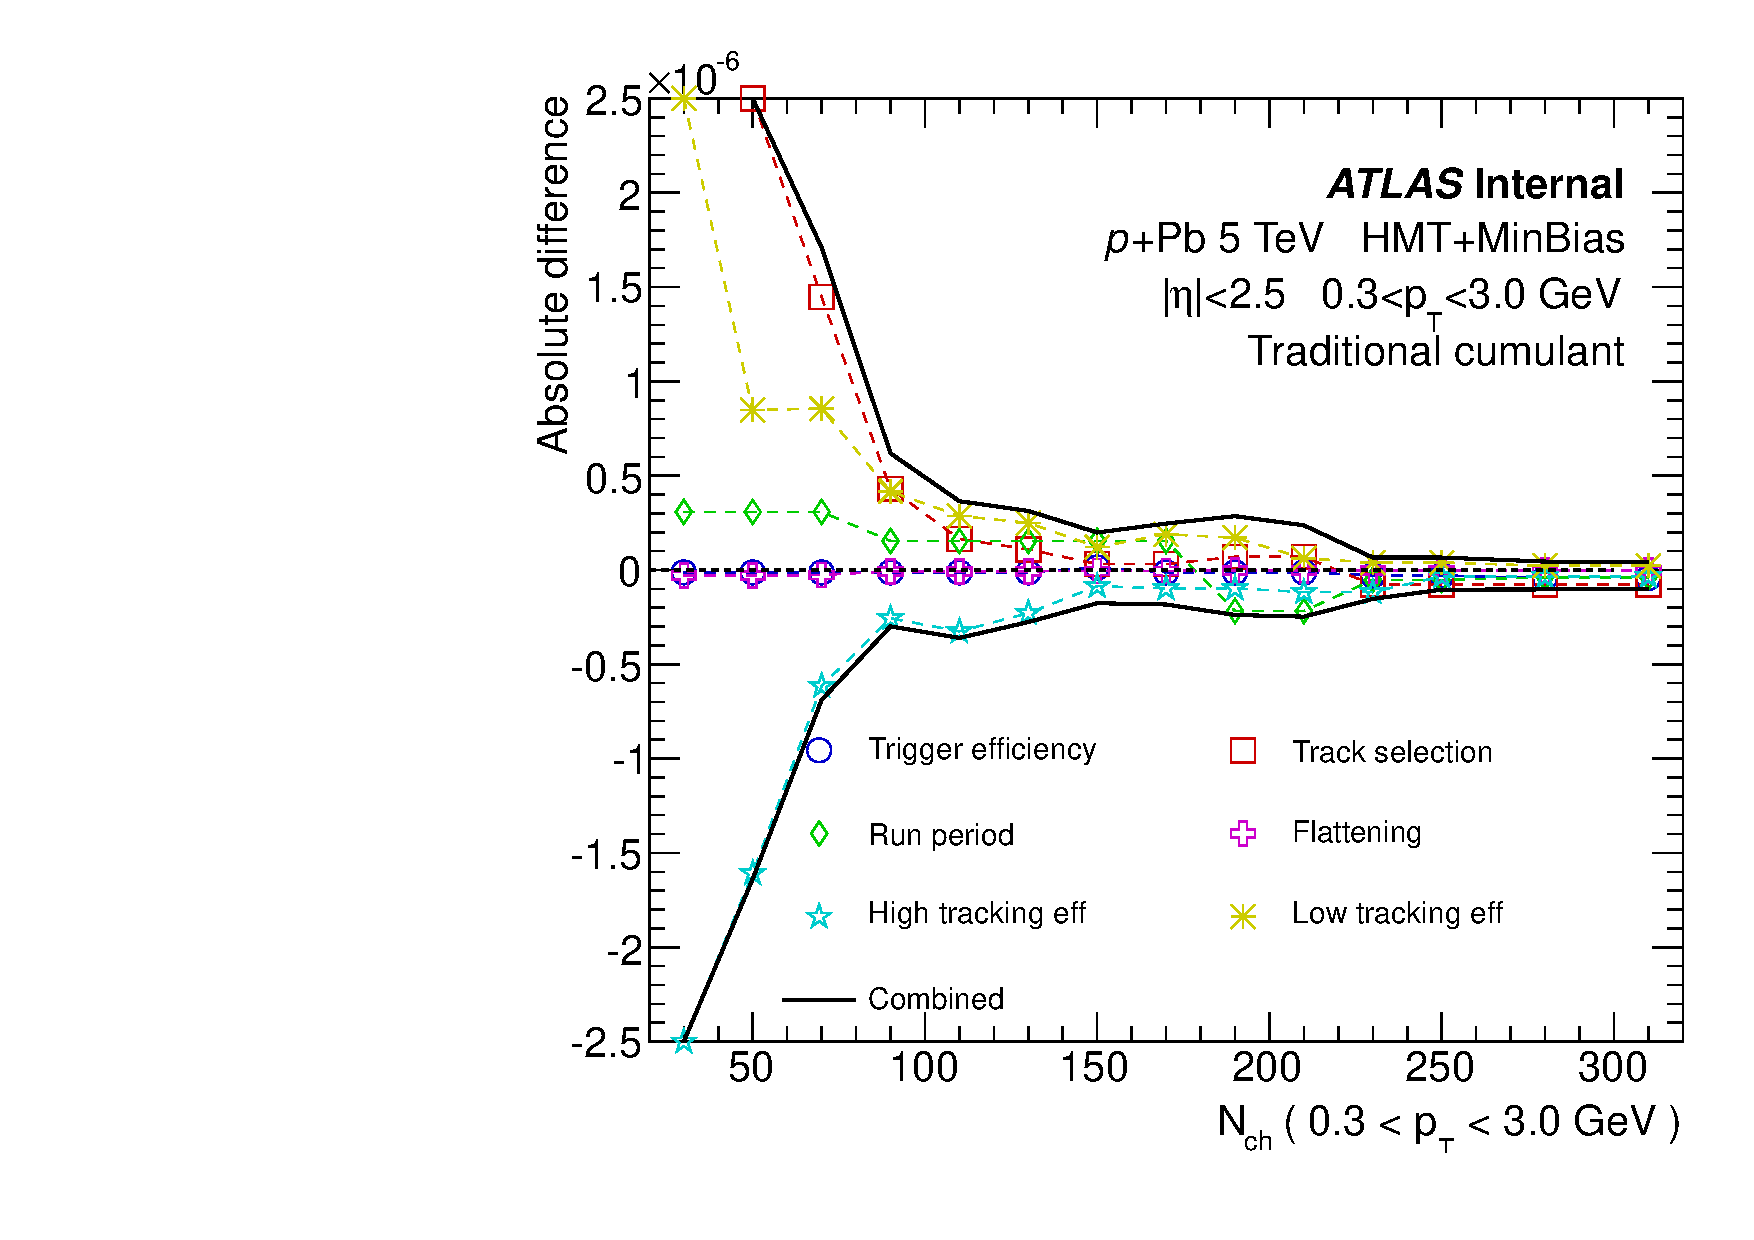
\includegraphics[width=0.3\linewidth]{figs/sec_sys/pPb5/sys_pPb5_NNNN_Har0_Pt0_Cls0.pdf}
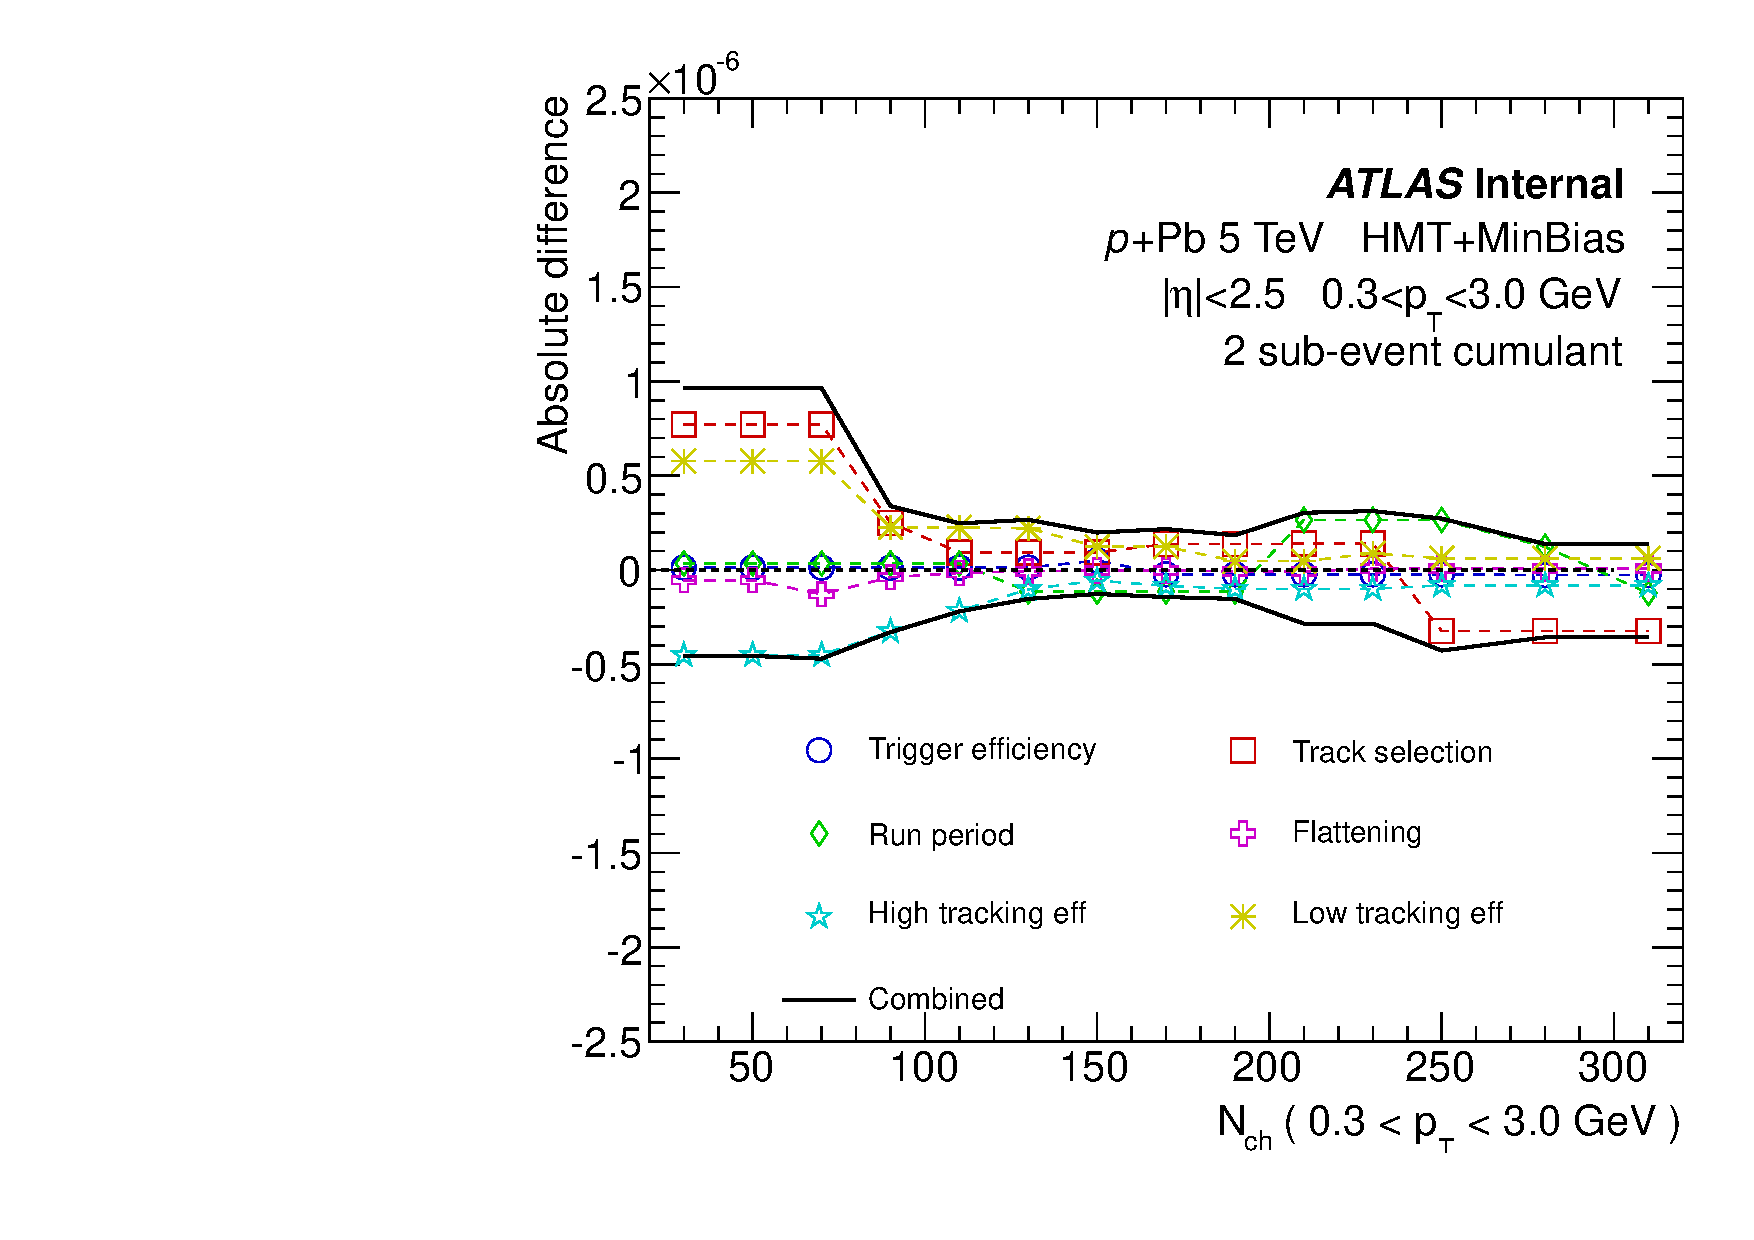
\includegraphics[width=0.3\linewidth]{figs/sec_sys/pPb5/sys_pPb5_ABAB_Har0_Pt0_Cls0.pdf}
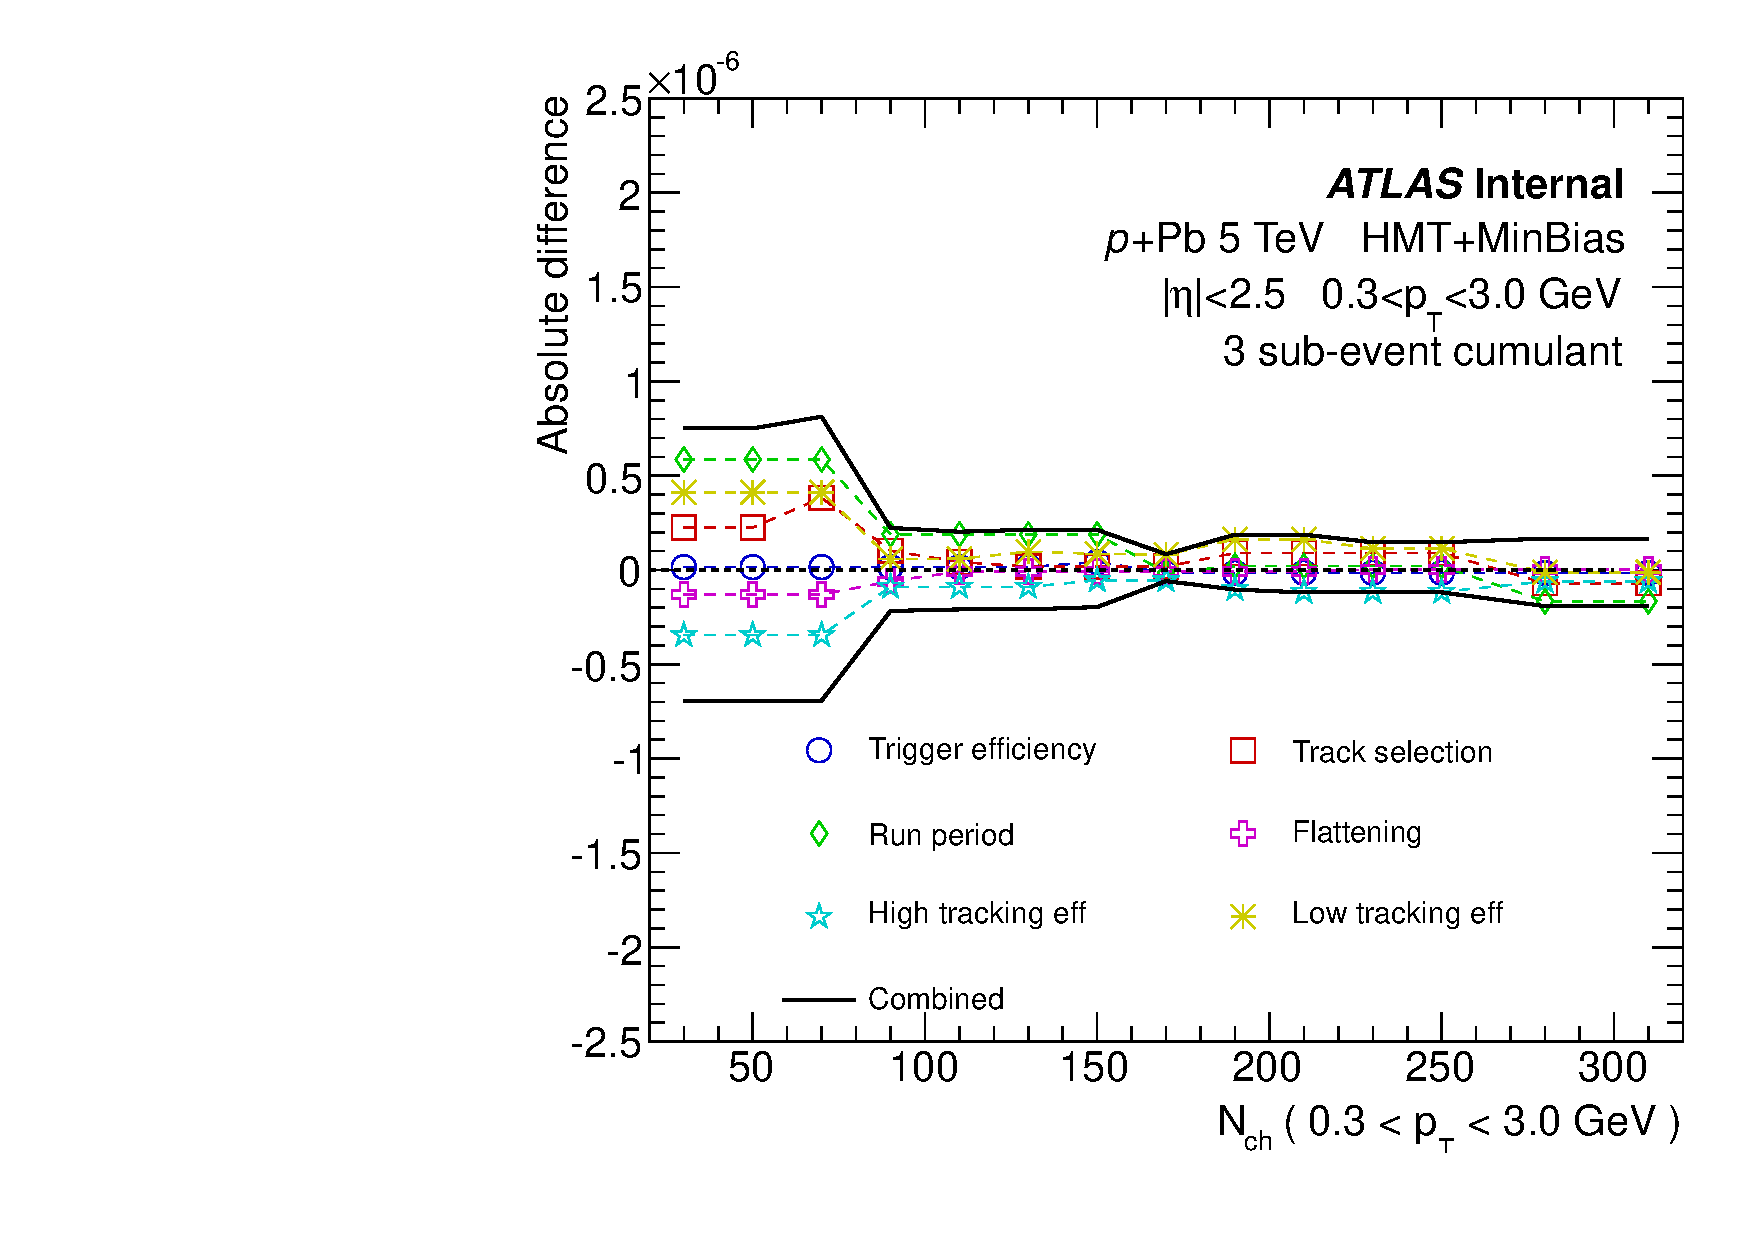
\includegraphics[width=0.3\linewidth]{figs/sec_sys/pPb5/sys_pPb5_ABAC_Har0_Pt0_Cls0.pdf}
\caption{Summary of systematics in 5.02 TeV $pPb$, for three different cumulant methods, with $0.3<p_{T}<3.0$ GeV. The statistical errors are not shown for better readability.}
\label{fig:sys_pPb5_sum_pt0}
\end{figure}

\begin{figure}[H]
\centering
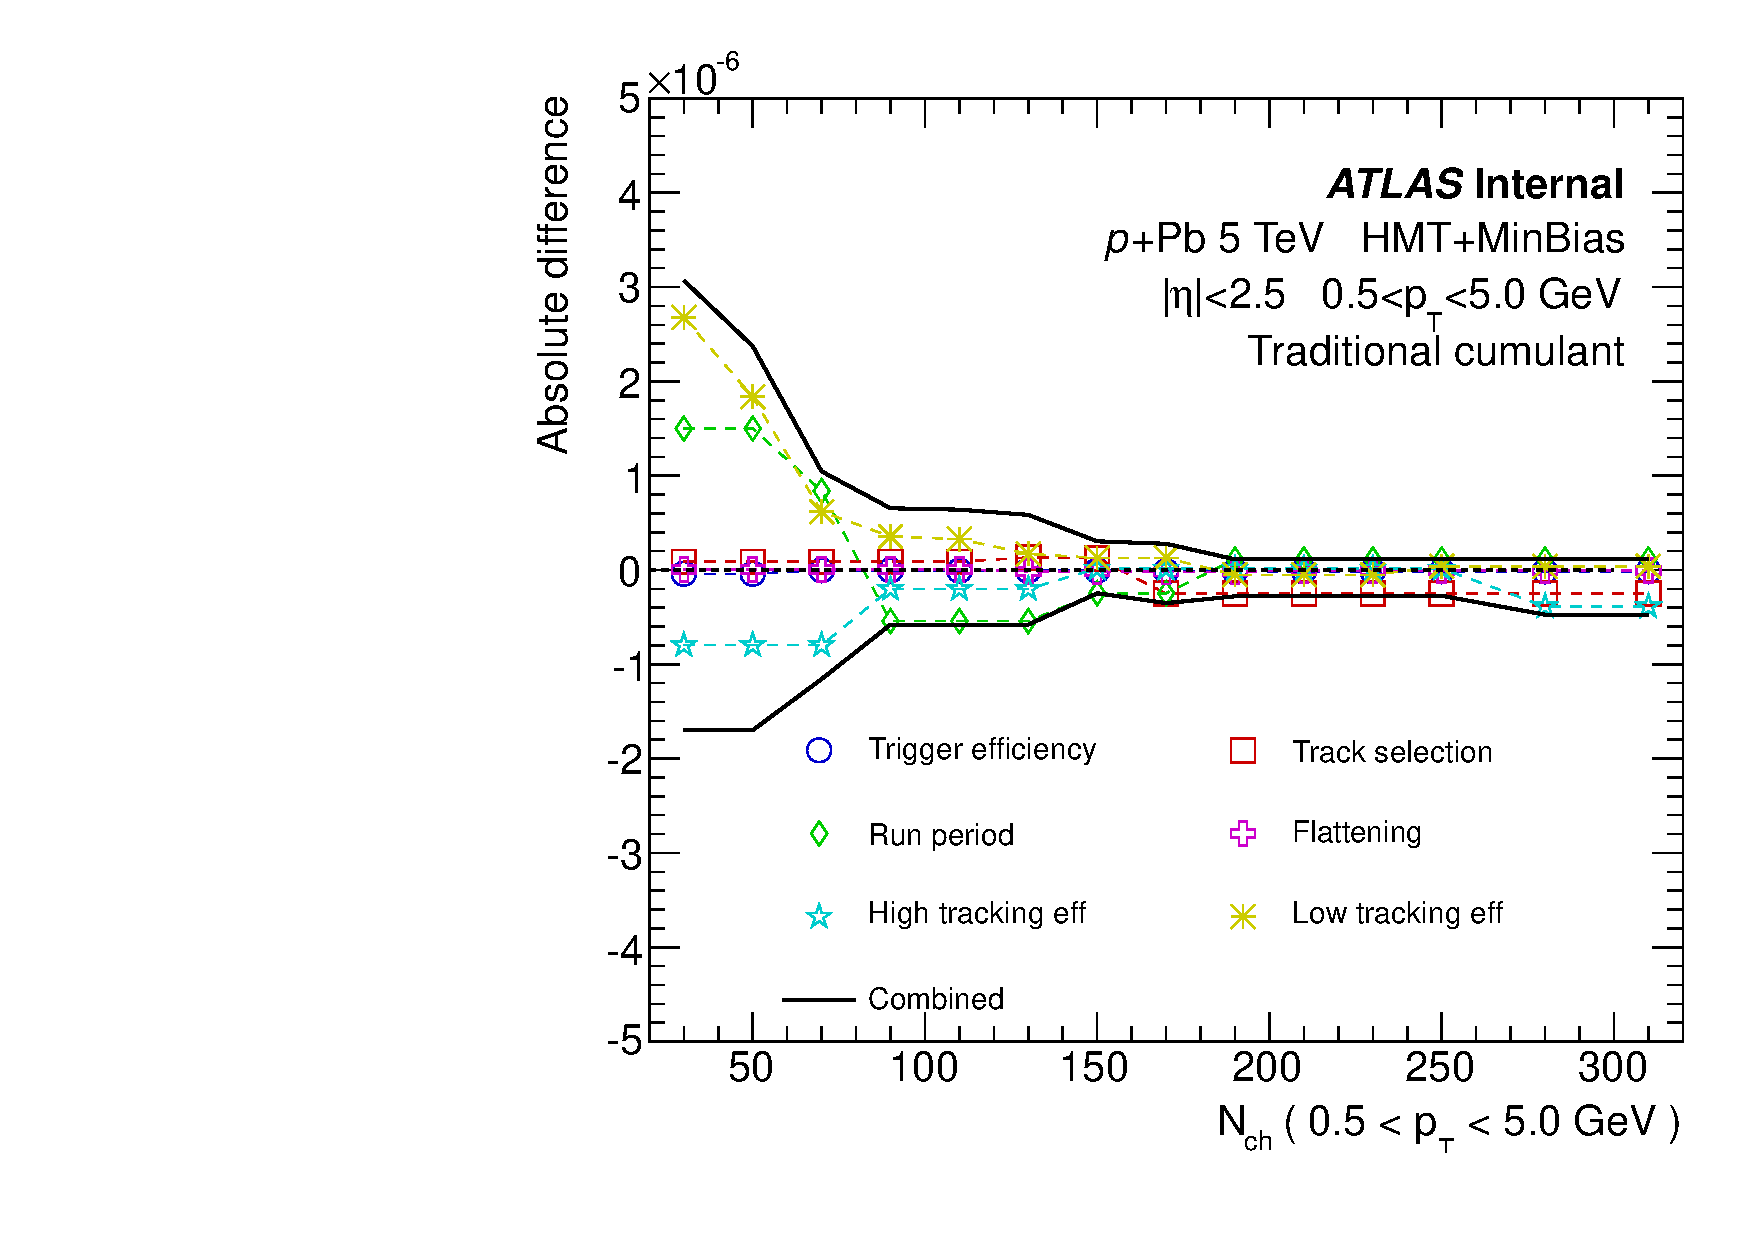
\includegraphics[width=0.3\linewidth]{figs/sec_sys/pPb5/sys_pPb5_NNNN_Har0_Pt1_Cls0.pdf}
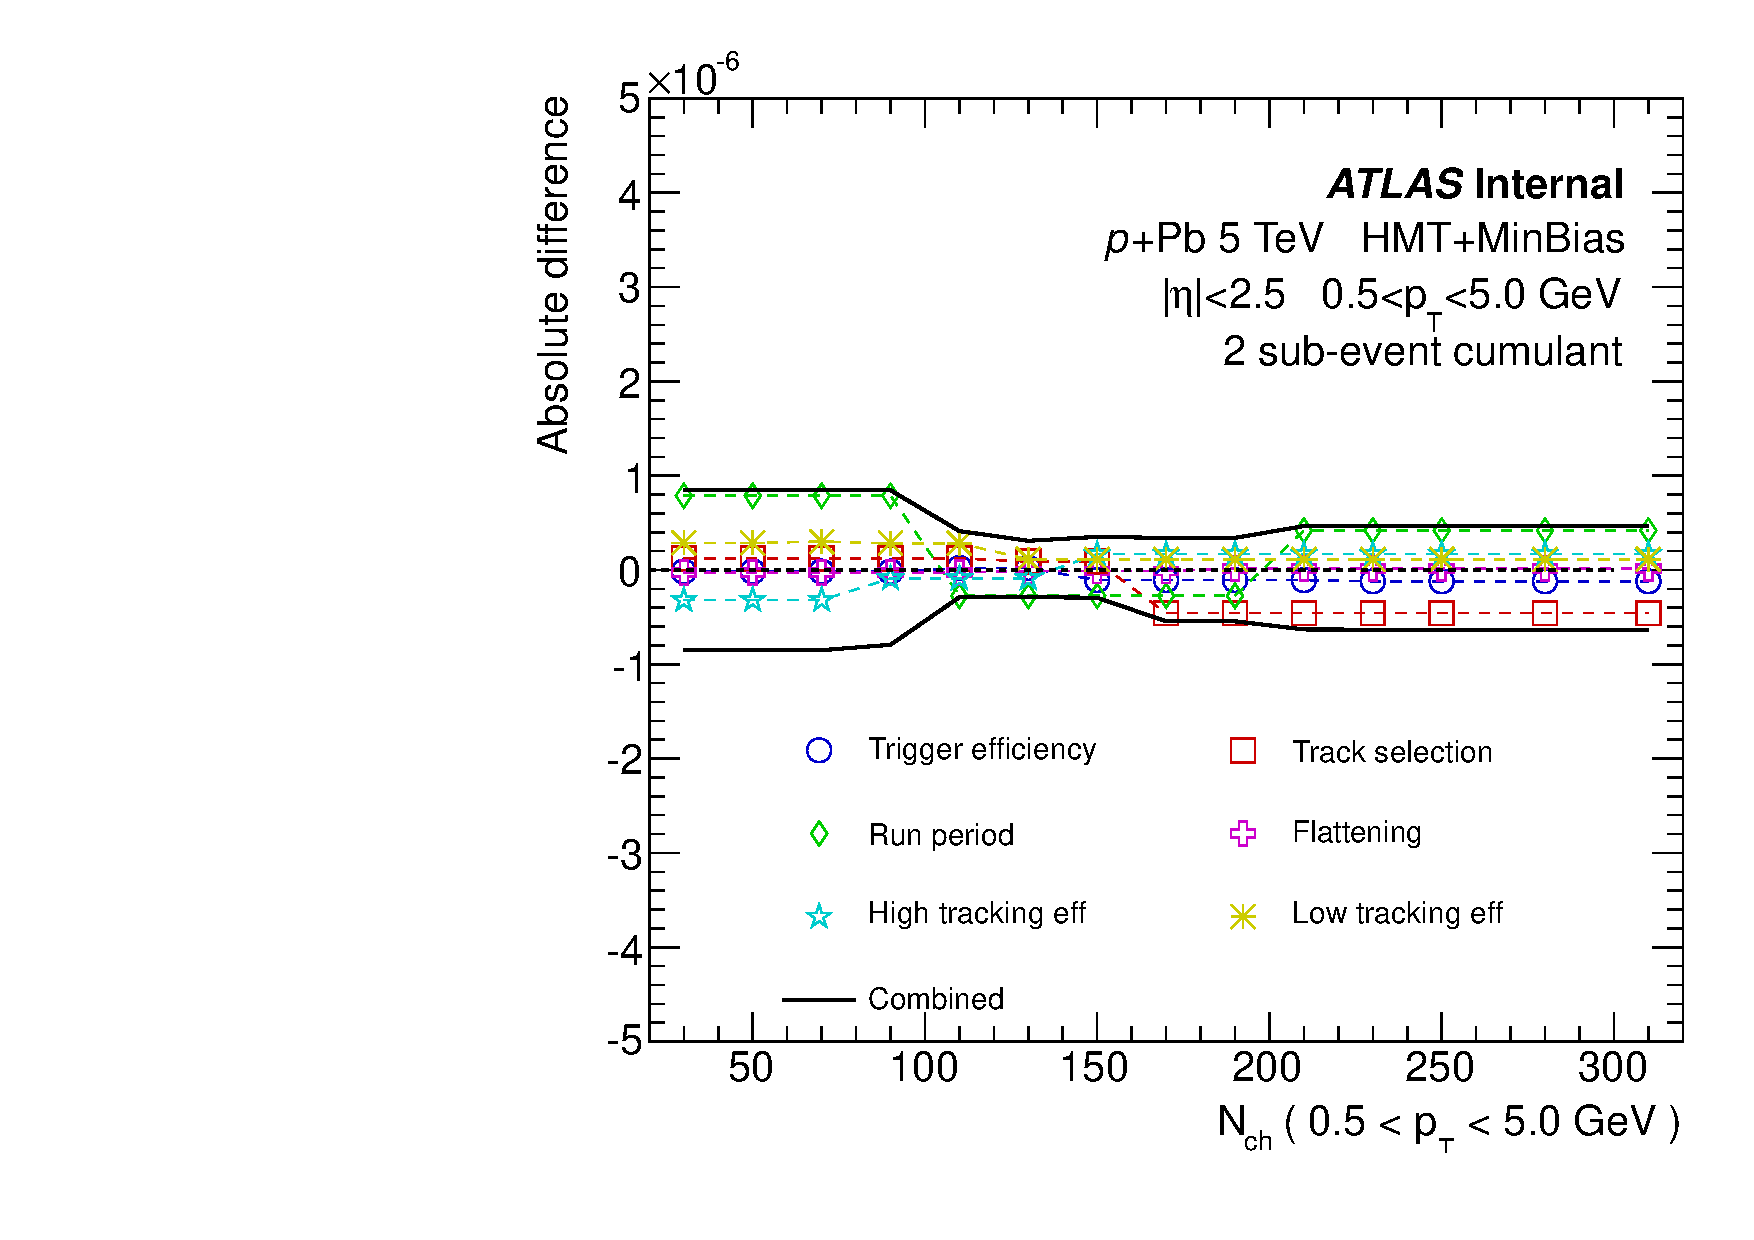
\includegraphics[width=0.3\linewidth]{figs/sec_sys/pPb5/sys_pPb5_ABAB_Har0_Pt1_Cls0.pdf}
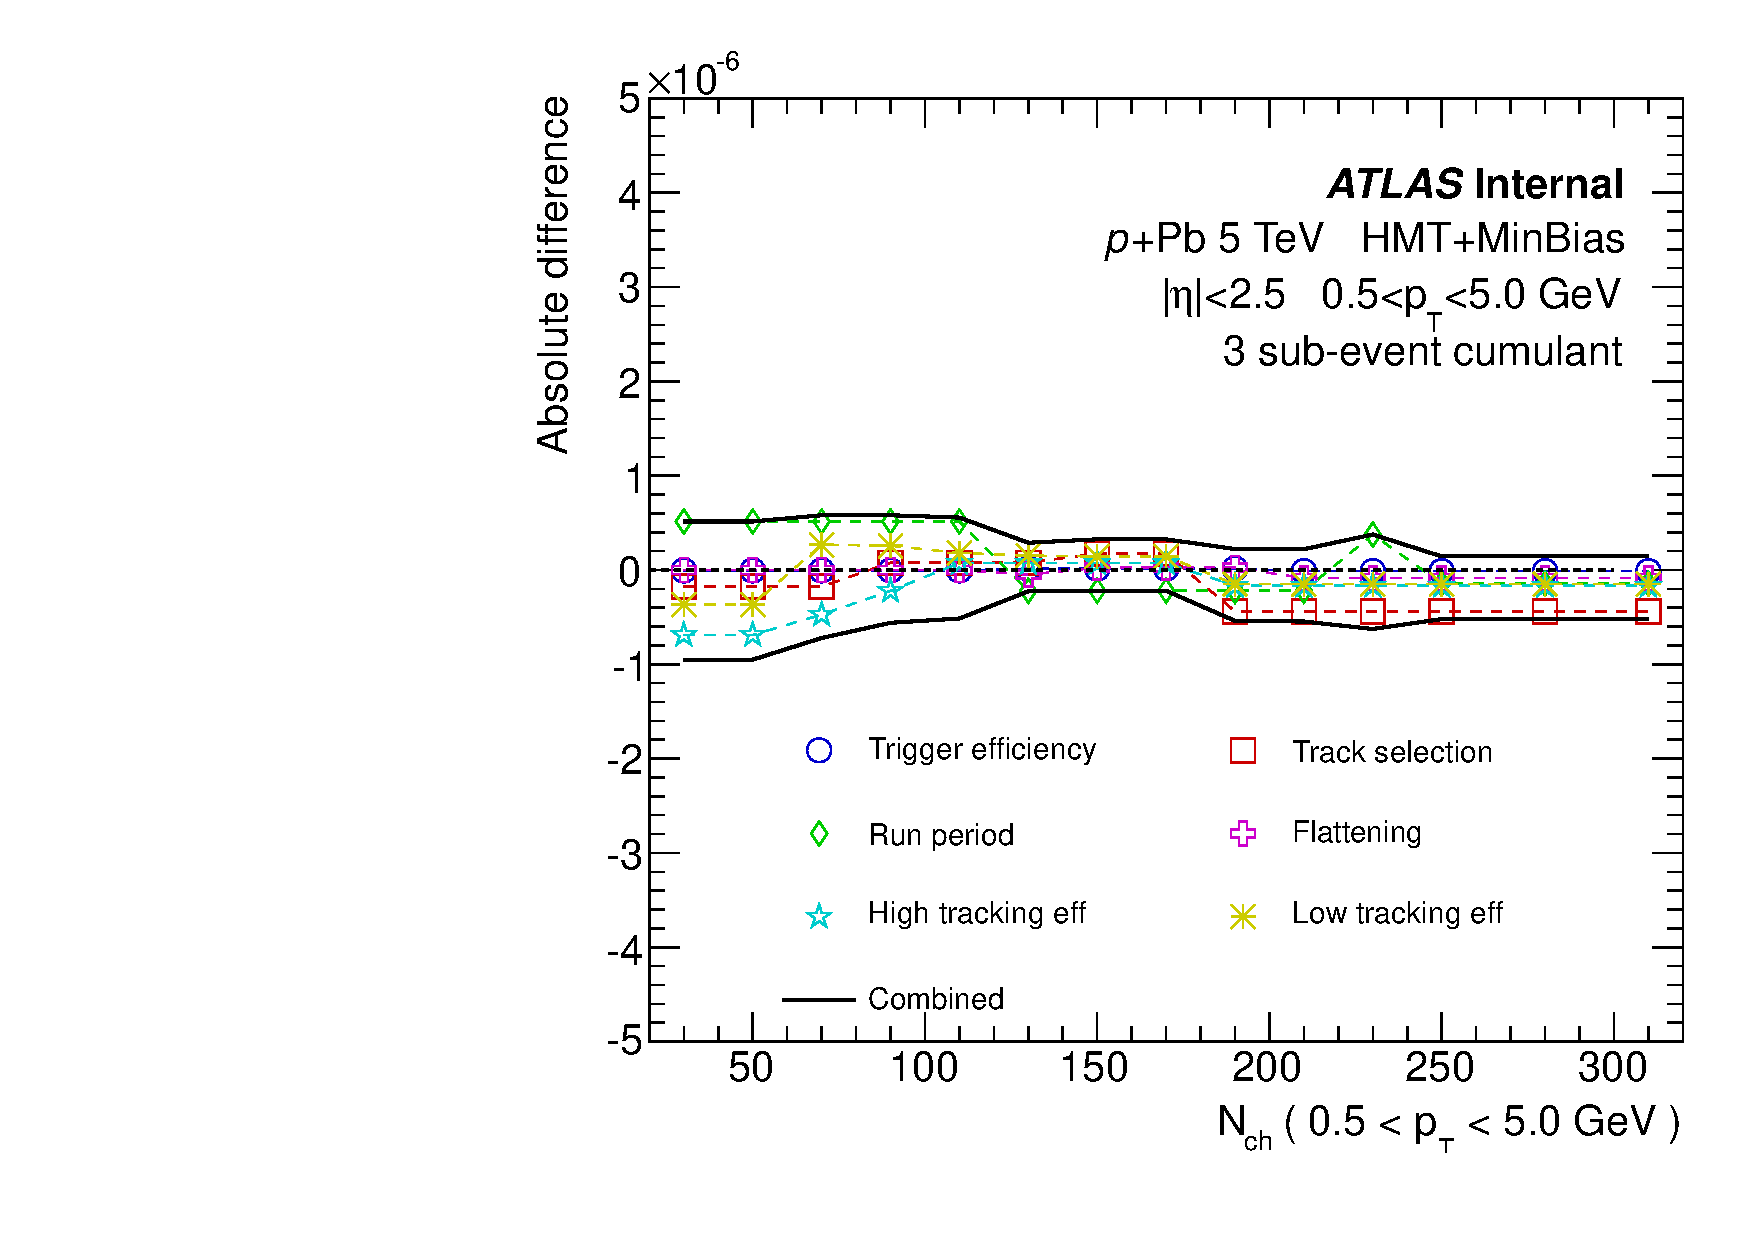
\includegraphics[width=0.3\linewidth]{figs/sec_sys/pPb5/sys_pPb5_ABAC_Har0_Pt1_Cls0.pdf}
\caption{Summary of systematics in 5.02 TeV $pPb$, for three different cumulant methods, with $0.5<p_{T}<5.0$ GeV. The statistical errors are not shown for better readability.}
\label{fig:sys_pPb5_sum_pt1}
\end{figure}






\subsection{Summary of systematic table}
The systematics of three collision systems, three cumulant methods and two $p_{\text{T}}$ ranges are summarized in Fig.~\ref{fig:systematic_table}, as a function of $N_{ch}$.
\begin{figure}[H]
\centering
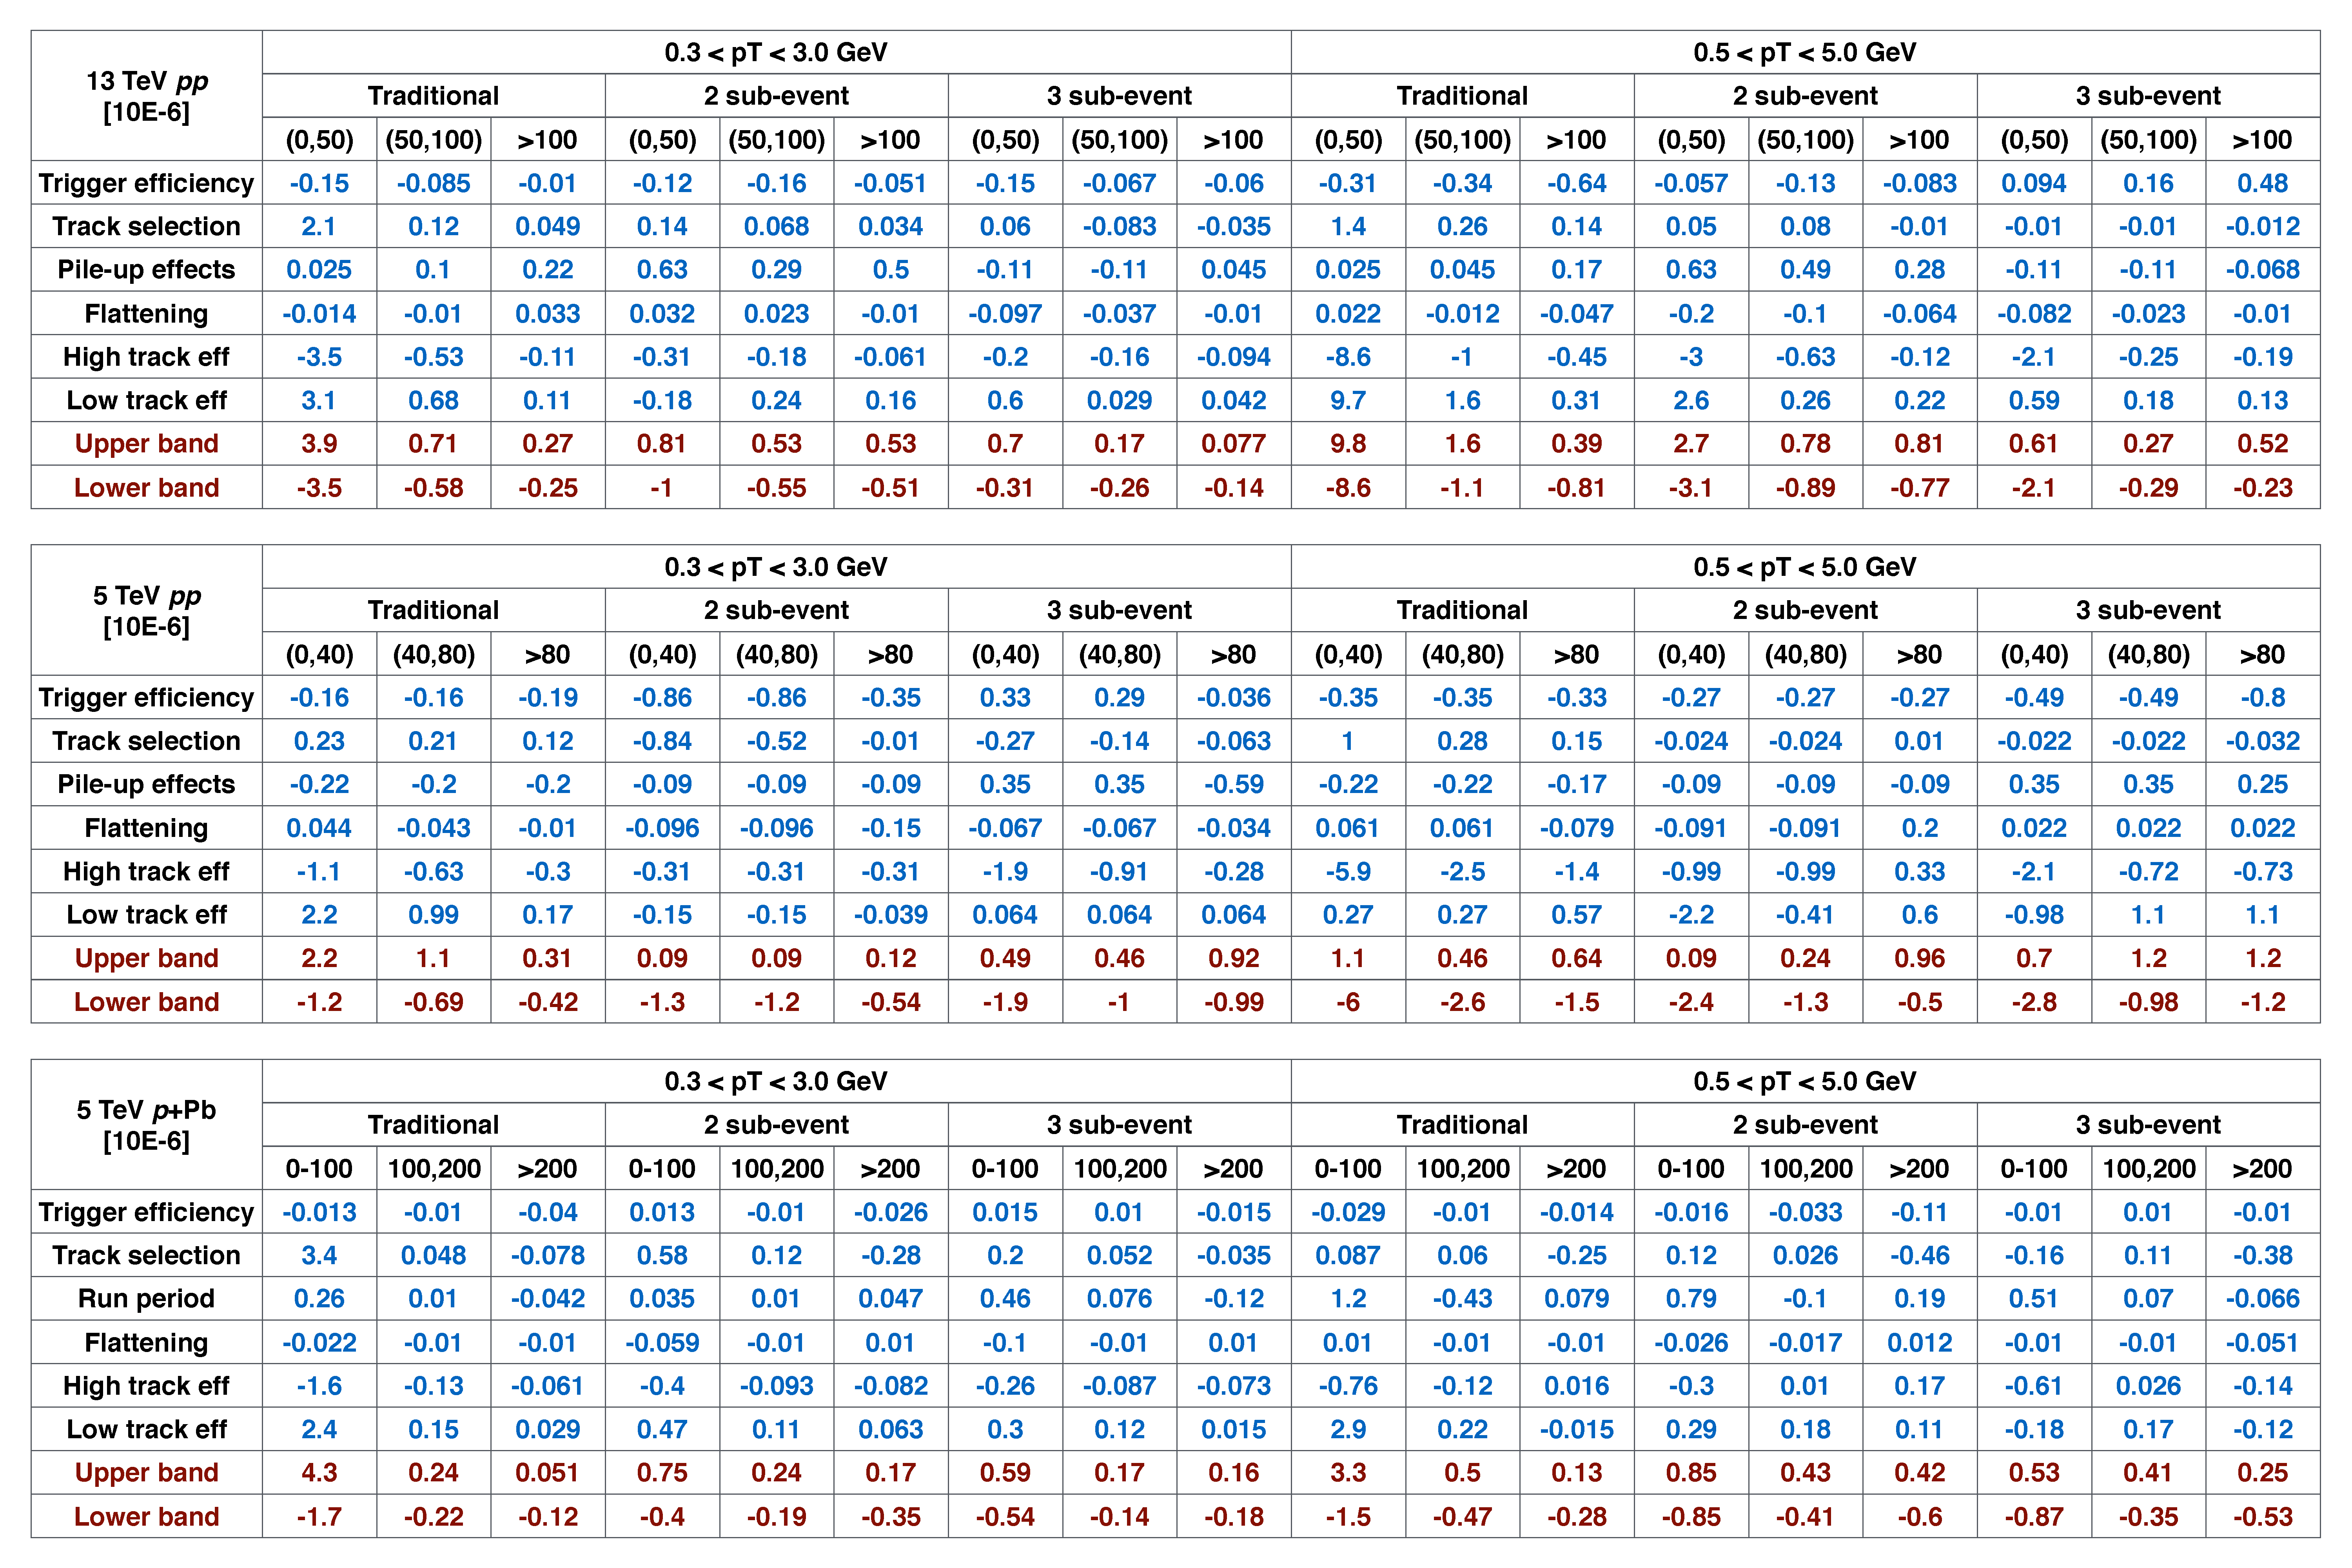
\includegraphics[width=1.\linewidth]{figs/sec_sys/systematic_table.pdf}
\caption{Summary of systematic table of three collision systems, three cumulant methods and two $p_{\text{T}}$ ranges, as a function of $N_{ch}$. The values in the table are absolute differences of each check, in the unit of $10^-6$.}
\label{fig:systematic_table}
\end{figure}



